\documentclass[10pt,a4paper]{article}
\usepackage[margin=2.2cm]{geometry}
\usepackage{amsmath,amssymb,amsthm,booktabs,graphicx,microtype,siunitx}
\usepackage[table]{xcolor}
\usepackage[round,authoryear]{natbib}
\usepackage[hidelinks]{hyperref}
\usepackage{caption}
\usepackage{times}
\usepackage[section]{placeins}
\captionsetup{font=small,labelfont=bf}
\sisetup{detect-all}
\newtheorem{proposition}{Proposition}
\newcommand{\zv}{\mathbf{z}}
\newcommand{\V}[1]{\csname v#1\endcsname}
\expandafter\def\csname vnruns\endcsname{132}
\expandafter\def\csname vgpuh\endcsname{204}
\expandafter\def\csname vspread64\endcsname{0.250}
\expandafter\def\csname vseedsd64\endcsname{0.238}
\expandafter\def\csname vanovaF\endcsname{0.954}
\expandafter\def\csname vanovaP\endcsname{0.450}
\expandafter\def\csname vanovaEta\endcsname{0.132}
\expandafter\def\csname vw64uniformd\endcsname{+0.048}
\expandafter\def\csname vw64uniformtost\endcsname{0.0142}
\expandafter\def\csname vw64gapd\endcsname{+0.080}
\expandafter\def\csname vw64gaptost\endcsname{0.0188}
\expandafter\def\csname vw64shuffledd\endcsname{-0.073}
\expandafter\def\csname vw64shuffledtost\endcsname{0.0464}
\expandafter\def\csname vw64frozenrandomd\endcsname{+0.177}
\expandafter\def\csname vw64frozenrandomtost\endcsname{0.0191}
\expandafter\def\csname vfrzVgap\endcsname{+0.097}
\expandafter\def\csname vfrzVgapP\endcsname{0.443}
\expandafter\def\csname vfrzVgapT\endcsname{0.0089}
\expandafter\def\csname vgapEntMin\endcsname{0.9867}
\expandafter\def\csname vgapEntMean\endcsname{0.9885}
\expandafter\def\csname vpowsd\endcsname{0.257}
\expandafter\def\csname vmde\endcsname{0.270}
\expandafter\def\csname vpwA\endcsname{48.5}
\expandafter\def\csname vpwB\endcsname{96.3}
\expandafter\def\csname vpwC\endcsname{100.0}
\expandafter\def\csname veffCA\endcsname{+0.532}
\expandafter\def\csname veffCAlo\endcsname{+0.292}
\expandafter\def\csname veffCAhi\endcsname{+0.771}
\expandafter\def\csname veffCAp\endcsname{=0.0023}
\expandafter\def\csname vbankCA\endcsname{-0.223}
\expandafter\def\csname vbankCAT\endcsname{0.0251}
\expandafter\def\csname vroutCA\endcsname{+0.755}
\expandafter\def\csname vlossCA\endcsname{0.1643}
\expandafter\def\csname veffCB\endcsname{+1.153}
\expandafter\def\csname veffCBlo\endcsname{+0.940}
\expandafter\def\csname veffCBhi\endcsname{+1.367}
\expandafter\def\csname veffCBp\endcsname{<10^{-4}}
\expandafter\def\csname vbankCB\endcsname{+0.175}
\expandafter\def\csname vbankCBT\endcsname{0.0242}
\expandafter\def\csname vroutCB\endcsname{+0.978}
\expandafter\def\csname vlossCB\endcsname{0.0170}
\expandafter\def\csname veffCC\endcsname{+0.080}
\expandafter\def\csname veffCClo\endcsname{-0.305}
\expandafter\def\csname veffCChi\endcsname{+0.465}
\expandafter\def\csname veffCCp\endcsname{=0.6158}
\expandafter\def\csname vbankCC\endcsname{+0.048}
\expandafter\def\csname vbankCCT\endcsname{0.0142}
\expandafter\def\csname vroutCC\endcsname{+0.032}
\expandafter\def\csname vlossCC\endcsname{0.0080}
\expandafter\def\csname veffTA\endcsname{+2.185}
\expandafter\def\csname veffTAlo\endcsname{+1.781}
\expandafter\def\csname veffTAhi\endcsname{+2.589}
\expandafter\def\csname veffTAp\endcsname{<10^{-4}}
\expandafter\def\csname vbankTA\endcsname{+0.107}
\expandafter\def\csname vbankTAT\endcsname{0.0218}
\expandafter\def\csname vroutTA\endcsname{+2.078}
\expandafter\def\csname vlossTA\endcsname{0.1194}
\expandafter\def\csname veffTB\endcsname{+2.282}
\expandafter\def\csname veffTBlo\endcsname{+1.952}
\expandafter\def\csname veffTBhi\endcsname{+2.611}
\expandafter\def\csname veffTBp\endcsname{<10^{-4}}
\expandafter\def\csname vbankTB\endcsname{+0.053}
\expandafter\def\csname vbankTBT\endcsname{0.0157}
\expandafter\def\csname vroutTB\endcsname{+2.228}
\expandafter\def\csname vlossTB\endcsname{0.0210}
\expandafter\def\csname vmMA\endcsname{+4.345}
\expandafter\def\csname vmMAlo\endcsname{+4.103}
\expandafter\def\csname vmMAhi\endcsname{+4.587}
\expandafter\def\csname vtMAg\endcsname{33.7}
\expandafter\def\csname vtMAs\endcsname{8.6}
\expandafter\def\csname vmMB\endcsname{+2.313}
\expandafter\def\csname vmMBlo\endcsname{+1.870}
\expandafter\def\csname vmMBhi\endcsname{+2.757}
\expandafter\def\csname vtMBg\endcsname{39.2}
\expandafter\def\csname vtMBs\endcsname{18.8}
\expandafter\def\csname vmMC\endcsname{+2.520}
\expandafter\def\csname vmMClo\endcsname{+2.311}
\expandafter\def\csname vmMChi\endcsname{+2.729}
\expandafter\def\csname vtMCg\endcsname{284.2}
\expandafter\def\csname vtMCs\endcsname{129.0}
\expandafter\def\csname vk8vs64\endcsname{2.29}
\expandafter\def\csname vk82\endcsname{+0.098}
\expandafter\def\csname vk82p\endcsname{0.409}
\expandafter\def\csname vkpar\endcsname{3.9}
\expandafter\def\csname vktime\endcsname{2.5}
\expandafter\def\csname vpredP\endcsname{1.0\times10^{-5}}
\expandafter\def\csname vtin64r\endcsname{97.7}
\expandafter\def\csname vanA\endcsname{+0.115}
\expandafter\def\csname vanAp\endcsname{0.4313}
\expandafter\def\csname vansA\endcsname{+0.647}
\expandafter\def\csname vansAT\endcsname{0.8259}
\expandafter\def\csname vanuA\endcsname{+0.870}
\expandafter\def\csname vanuAp\endcsname{0.0044}
\expandafter\def\csname vanuAT\endcsname{0.9545}
\expandafter\def\csname vhcA\endcsname{0.03983}
\expandafter\def\csname vhaA\endcsname{0.00282}
\expandafter\def\csname vflA\endcsname{14}
\expandafter\def\csname vlaA\endcsname{0.1540}
\expandafter\def\csname vlcA\endcsname{0.0638}
\expandafter\def\csname vbcA\endcsname{+0.755}
\expandafter\def\csname vanB\endcsname{-0.682}
\expandafter\def\csname vanBp\endcsname{0.0017}
\expandafter\def\csname vansB\endcsname{+0.472}
\expandafter\def\csname vansBT\endcsname{0.4319}
\expandafter\def\csname vanuB\endcsname{+0.297}
\expandafter\def\csname vanuBp\endcsname{0.0810}
\expandafter\def\csname vanuBT\endcsname{0.0976}
\expandafter\def\csname vhcB\endcsname{0.02132}
\expandafter\def\csname vhaB\endcsname{0.00073}
\expandafter\def\csname vflB\endcsname{29}
\expandafter\def\csname vlaB\endcsname{0.0173}
\expandafter\def\csname vlcB\endcsname{0.0132}
\expandafter\def\csname vbcB\endcsname{+0.978}
\expandafter\def\csname vanC\endcsname{-0.048}
\expandafter\def\csname vanCp\endcsname{0.7449}
\expandafter\def\csname vansC\endcsname{+0.032}
\expandafter\def\csname vansCT\endcsname{0.0025}
\expandafter\def\csname vanuC\endcsname{-0.017}
\expandafter\def\csname vanuCp\endcsname{0.8369}
\expandafter\def\csname vanuCT\endcsname{0.0007}
\expandafter\def\csname vhcC\endcsname{0.01147}
\expandafter\def\csname vhaC\endcsname{0.00018}
\expandafter\def\csname vflC\endcsname{63}
\expandafter\def\csname vlaC\endcsname{0.0080}
\expandafter\def\csname vlcC\endcsname{0.0074}
\expandafter\def\csname vbcC\endcsname{+0.032}
\expandafter\def\csname vconstT64\endcsname{0.0188}
\expandafter\def\csname vspanlo\endcsname{0.228}
\expandafter\def\csname vspanhi\endcsname{0.272}
\expandafter\def\csname vspanpct\endcsname{9}
\expandafter\def\csname vmbruns\endcsname{132}
\expandafter\def\csname vmbgpuh\endcsname{254}
\expandafter\def\csname vtotruns\endcsname{396}
\expandafter\def\csname vtotgpuh\endcsname{564}
\expandafter\def\csname vtwogpuh\endcsname{458}
\expandafter\def\csname vvgruns\endcsname{132}
\expandafter\def\csname vvggpuh\endcsname{106}
\expandafter\def\csname vvggate\endcsname{74.68}
\expandafter\def\csname vvgpstatic\endcsname{14.77}
\expandafter\def\csname vvgrouterK\endcsname{392}
\expandafter\def\csname vvgrouterpct\endcsname{2.7}
\expandafter\def\csname vvgbankadd\endcsname{44.13}
\expandafter\def\csname vvgdynshare\endcsname{100}
\expandafter\def\csname vvgnlayers\endcsname{12}
\expandafter\def\csname vvgmicro\endcsname{128}
\expandafter\def\csname vvgbankCA\endcsname{+0.145}
\expandafter\def\csname vvgbankCAT\endcsname{0.0621}
\expandafter\def\csname vvgbankCAv\endcsname{inconclusive}
\expandafter\def\csname vvgroutCA\endcsname{+0.718}
\expandafter\def\csname vvgroutCAp\endcsname{0.0375}
\expandafter\def\csname vvgroutCAv\endcsname{higher}
\expandafter\def\csname vvgeffCA\endcsname{+0.863}
\expandafter\def\csname vvgeffCAlo\endcsname{+0.486}
\expandafter\def\csname vvgeffCAhi\endcsname{+1.240}
\expandafter\def\csname vvgeffCAp\endcsname{0.0020}
\expandafter\def\csname vvgeffCAT\endcsname{0.9720}
\expandafter\def\csname vvgeffCAv\endcsname{higher}
\expandafter\def\csname vvgbankCB\endcsname{-0.148}
\expandafter\def\csname vvgbankCBT\endcsname{0.0834}
\expandafter\def\csname vvgbankCBv\endcsname{inconclusive}
\expandafter\def\csname vvgroutCB\endcsname{+0.627}
\expandafter\def\csname vvgroutCBp\endcsname{0.0569}
\expandafter\def\csname vvgroutCBv\endcsname{inconclusive}
\expandafter\def\csname vvgeffCB\endcsname{+0.478}
\expandafter\def\csname vvgeffCBlo\endcsname{+0.193}
\expandafter\def\csname vvgeffCBhi\endcsname{+0.764}
\expandafter\def\csname vvgeffCBp\endcsname{0.0077}
\expandafter\def\csname vvgeffCBT\endcsname{0.4265}
\expandafter\def\csname vvgeffCBv\endcsname{higher}
\expandafter\def\csname vvgbankCC\endcsname{-0.188}
\expandafter\def\csname vvgbankCCT\endcsname{0.0147}
\expandafter\def\csname vvgbankCCv\endcsname{equivalent}
\expandafter\def\csname vvgroutCC\endcsname{+0.373}
\expandafter\def\csname vvgroutCCp\endcsname{0.0025}
\expandafter\def\csname vvgroutCCv\endcsname{higher}
\expandafter\def\csname vvgeffCC\endcsname{+0.185}
\expandafter\def\csname vvgeffCClo\endcsname{-0.029}
\expandafter\def\csname vvgeffCChi\endcsname{+0.399}
\expandafter\def\csname vvgeffCCp\endcsname{0.0766}
\expandafter\def\csname vvgeffCCT\endcsname{0.0064}
\expandafter\def\csname vvgeffCCv\endcsname{equivalent}
\expandafter\def\csname vvgbankTA\endcsname{+0.128}
\expandafter\def\csname vvgbankTAT\endcsname{0.0039}
\expandafter\def\csname vvgbankTAv\endcsname{equivalent}
\expandafter\def\csname vvgroutTA\endcsname{+1.637}
\expandafter\def\csname vvgroutTAp\endcsname{0.0001}
\expandafter\def\csname vvgroutTAv\endcsname{higher}
\expandafter\def\csname vvgeffTA\endcsname{+1.765}
\expandafter\def\csname vvgeffTAlo\endcsname{+1.365}
\expandafter\def\csname vvgeffTAhi\endcsname{+2.165}
\expandafter\def\csname vvgeffTAp\endcsname{$<10^{-4}$}
\expandafter\def\csname vvgeffTAT\endcsname{0.9998}
\expandafter\def\csname vvgeffTAv\endcsname{higher}
\expandafter\def\csname vvgbankTB\endcsname{+0.250}
\expandafter\def\csname vvgbankTBT\endcsname{0.1458}
\expandafter\def\csname vvgbankTBv\endcsname{inconclusive}
\expandafter\def\csname vvgroutTB\endcsname{+1.230}
\expandafter\def\csname vvgroutTBp\endcsname{0.0055}
\expandafter\def\csname vvgroutTBv\endcsname{higher}
\expandafter\def\csname vvgeffTB\endcsname{+1.480}
\expandafter\def\csname vvgeffTBlo\endcsname{+0.812}
\expandafter\def\csname vvgeffTBhi\endcsname{+2.148}
\expandafter\def\csname vvgeffTBp\endcsname{0.0023}
\expandafter\def\csname vvgeffTBT\endcsname{0.9935}
\expandafter\def\csname vvgeffTBv\endcsname{higher}
\expandafter\def\csname vvgnbankeq\endcsname{2}
\expandafter\def\csname vvgnbanksig\endcsname{0}
\expandafter\def\csname vvgnrout\endcsname{4}
\expandafter\def\csname vvgneff\endcsname{4}
\expandafter\def\csname vvgbankmax\endcsname{+0.25}
\expandafter\def\csname vvgnresumed\endcsname{1}
\expandafter\def\csname vvgresumedseed\endcsname{0}
\expandafter\def\csname vvgresumedacc\endcsname{74.55}
\expandafter\def\csname vvgsensS\endcsname{-0.254}
\expandafter\def\csname vvgsensSp\endcsname{0.2451}
\expandafter\def\csname vvgsensSv\endcsname{inconclusive}
\expandafter\def\csname vvgsensG\endcsname{-0.474}
\expandafter\def\csname vvgsensGp\endcsname{0.0330}
\expandafter\def\csname vvgsensGv\endcsname{lower}
\expandafter\def\csname vvgwuniformstatic\endcsname{-0.188}
\expandafter\def\csname vvgwuniformstaticlo\endcsname{-0.453}
\expandafter\def\csname vvgwuniformstatichi\endcsname{+0.077}
\expandafter\def\csname vvgwuniformstaticp\endcsname{0.1273}
\expandafter\def\csname vvgwuniformstaticT\endcsname{0.0147}
\expandafter\def\csname vvgwuniformstaticv\endcsname{equivalent}
\expandafter\def\csname vvgwgapstatic\endcsname{+0.185}
\expandafter\def\csname vvgwgapstaticlo\endcsname{-0.029}
\expandafter\def\csname vvgwgapstatichi\endcsname{+0.399}
\expandafter\def\csname vvgwgapstaticp\endcsname{0.0766}
\expandafter\def\csname vvgwgapstaticT\endcsname{0.0064}
\expandafter\def\csname vvgwgapstaticv\endcsname{equivalent}
\expandafter\def\csname vvgwshuffledstatic\endcsname{-0.233}
\expandafter\def\csname vvgwshuffledstaticlo\endcsname{-0.629}
\expandafter\def\csname vvgwshuffledstatichi\endcsname{+0.162}
\expandafter\def\csname vvgwshuffledstaticp\endcsname{0.1896}
\expandafter\def\csname vvgwshuffledstaticT\endcsname{0.0717}
\expandafter\def\csname vvgwshuffledstaticv\endcsname{inconclusive}
\expandafter\def\csname vvgwfrozenrandomstatic\endcsname{-0.095}
\expandafter\def\csname vvgwfrozenrandomstaticlo\endcsname{-0.447}
\expandafter\def\csname vvgwfrozenrandomstatichi\endcsname{+0.257}
\expandafter\def\csname vvgwfrozenrandomstaticp\endcsname{0.5183}
\expandafter\def\csname vvgwfrozenrandomstaticT\endcsname{0.0157}
\expandafter\def\csname vvgwfrozenrandomstaticv\endcsname{equivalent}
\expandafter\def\csname vvgwfrozenrandomgap\endcsname{-0.280}
\expandafter\def\csname vvgwfrozenrandomgaplo\endcsname{-0.600}
\expandafter\def\csname vvgwfrozenrandomgaphi\endcsname{+0.040}
\expandafter\def\csname vvgwfrozenrandomgapp\endcsname{0.0743}
\expandafter\def\csname vvgwfrozenrandomgapT\endcsname{0.0687}
\expandafter\def\csname vvgwfrozenrandomgapv\endcsname{inconclusive}
\expandafter\def\csname vvgwshuffledgap\endcsname{-0.418}
\expandafter\def\csname vvgwshuffledgaplo\endcsname{-0.761}
\expandafter\def\csname vvgwshuffledgaphi\endcsname{-0.076}
\expandafter\def\csname vvgwshuffledgapp\endcsname{0.0257}
\expandafter\def\csname vvgwshuffledgapT\endcsname{0.2834}
\expandafter\def\csname vvgwshuffledgapv\endcsname{lower}
\expandafter\def\csname vvgwfrozenrandomuniform\endcsname{+0.093}
\expandafter\def\csname vvgwfrozenrandomuniformlo\endcsname{-0.120}
\expandafter\def\csname vvgwfrozenrandomuniformhi\endcsname{+0.306}
\expandafter\def\csname vvgwfrozenrandomuniformp\endcsname{0.3111}
\expandafter\def\csname vvgwfrozenrandomuniformT\endcsname{0.0022}
\expandafter\def\csname vvgwfrozenrandomuniformv\endcsname{equivalent}
\expandafter\def\csname vvgwgapuniform\endcsname{+0.373}
\expandafter\def\csname vvgwgapuniformlo\endcsname{+0.203}
\expandafter\def\csname vvgwgapuniformhi\endcsname{+0.544}
\expandafter\def\csname vvgwgapuniformp\endcsname{0.0025}
\expandafter\def\csname vvgwgapuniformT\endcsname{0.0572}
\expandafter\def\csname vvgwgapuniformv\endcsname{higher}
\expandafter\def\csname vvganovaF\endcsname{3.30}
\expandafter\def\csname vvganovaP\endcsname{0.027}
\expandafter\def\csname vvgspread64\endcsname{0.418}
\expandafter\def\csname vvgmMA\endcsname{+5.237}
\expandafter\def\csname vvgmMAp\endcsname{$<10^{-4}$}
\expandafter\def\csname vvgmMAr\endcsname{1.00}
\expandafter\def\csname vvgmMB\endcsname{+3.010}
\expandafter\def\csname vvgmMBp\endcsname{$<10^{-4}$}
\expandafter\def\csname vvgmMBr\endcsname{1.00}
\expandafter\def\csname vvgmMC\endcsname{+2.487}
\expandafter\def\csname vvgmMCp\endcsname{$<10^{-4}$}
\expandafter\def\csname vvgmMCr\endcsname{1.00}
\expandafter\def\csname vvgmmin\endcsname{2.5}
\expandafter\def\csname vvgmmax\endcsname{5.2}
\expandafter\def\csname vvgrlo\endcsname{1.00}
\expandafter\def\csname vvgrhi\endcsname{1.00}
\expandafter\def\csname vvgk2s\endcsname{+0.258}
\expandafter\def\csname vvgk2sp\endcsname{0.2978}
\expandafter\def\csname vvgk4s\endcsname{+0.478}
\expandafter\def\csname vvgk4sp\endcsname{0.0077}
\expandafter\def\csname vvgk8s\endcsname{+0.455}
\expandafter\def\csname vvgk8sp\endcsname{0.0189}
\expandafter\def\csname vvgnkbeat\endcsname{2}
\expandafter\def\csname vvgk82\endcsname{+0.197}
\expandafter\def\csname vvgk82p\endcsname{0.3928}
\expandafter\def\csname vvgk82v\endcsname{inconclusive}
\expandafter\def\csname vvgk82T\endcsname{0.1045}
\expandafter\def\csname vvganA\endcsname{-0.608}
\expandafter\def\csname vvganAp\endcsname{0.0075}
\expandafter\def\csname vvganuA\endcsname{+0.110}
\expandafter\def\csname vvganuAv\endcsname{inconclusive}
\expandafter\def\csname vvganuAp\endcsname{0.6023}
\expandafter\def\csname vvgansA\endcsname{+0.255}
\expandafter\def\csname vvgansAv\endcsname{equivalent}
\expandafter\def\csname vvgansAT\endcsname{0.0350}
\expandafter\def\csname vvglaA\endcsname{0.1003}
\expandafter\def\csname vvglcA\endcsname{0.0935}
\expandafter\def\csname vvganB\endcsname{-0.488}
\expandafter\def\csname vvganBp\endcsname{0.0409}
\expandafter\def\csname vvganuB\endcsname{+0.138}
\expandafter\def\csname vvganuBv\endcsname{equivalent}
\expandafter\def\csname vvganuBp\endcsname{0.4137}
\expandafter\def\csname vvgansB\endcsname{-0.010}
\expandafter\def\csname vvgansBv\endcsname{equivalent}
\expandafter\def\csname vvgansBT\endcsname{0.0027}
\expandafter\def\csname vvglaB\endcsname{0.0147}
\expandafter\def\csname vvglcB\endcsname{0.0145}
\expandafter\def\csname vvganC\endcsname{-0.202}
\expandafter\def\csname vvganCp\endcsname{0.0482}
\expandafter\def\csname vvganuC\endcsname{+0.172}
\expandafter\def\csname vvganuCv\endcsname{higher}
\expandafter\def\csname vvganuCp\endcsname{0.0044}
\expandafter\def\csname vvgansC\endcsname{-0.017}
\expandafter\def\csname vvgansCv\endcsname{equivalent}
\expandafter\def\csname vvgansCT\endcsname{0.0051}
\expandafter\def\csname vvglaC\endcsname{0.0058}
\expandafter\def\csname vvglcC\endcsname{0.0057}
\expandafter\def\csname vvgP1\endcsname{2}
\expandafter\def\csname vvgP2\endcsname{3}
\expandafter\def\csname vvgP3\endcsname{4}
\expandafter\def\csname vvgP1o\endcsname{failed}
\expandafter\def\csname vvgP2o\endcsname{held}
\expandafter\def\csname vvgP3o\endcsname{held}
\expandafter\def\csname vvglossCA\endcsname{0.1025}
\expandafter\def\csname vvglossCB\endcsname{0.0148}
\expandafter\def\csname vvglossCC\endcsname{0.0053}
\expandafter\def\csname vvglossTA\endcsname{0.0713}
\expandafter\def\csname vvglossTB\endcsname{0.0112}
\expandafter\def\csname vmbgate\endcsname{72.66}
\expandafter\def\csname vmbstatic\endcsname{72.39}
\expandafter\def\csname vmbpstatic\endcsname{2.35}
\expandafter\def\csname vmbpgap\endcsname{3.68}
\expandafter\def\csname vmbrouterK\endcsname{1137}
\expandafter\def\csname vmbrouterpct\endcsname{48}
\expandafter\def\csname vmbbankadd\endcsname{0.19}
\expandafter\def\csname vmbdynshare\endcsname{3}
\expandafter\def\csname vmbbankCA\endcsname{+0.593}
\expandafter\def\csname vmbbankCAT\endcsname{0.5884}
\expandafter\def\csname vmbroutCA\endcsname{+1.322}
\expandafter\def\csname vmbroutCAp\endcsname{0.0011}
\expandafter\def\csname vmbeffCA\endcsname{+1.915}
\expandafter\def\csname vmbeffCAlo\endcsname{+0.404}
\expandafter\def\csname vmbeffCAhi\endcsname{+3.426}
\expandafter\def\csname vmbeffCAp\endcsname{0.0225}
\expandafter\def\csname vmbbankCB\endcsname{-0.102}
\expandafter\def\csname vmbbankCBT\endcsname{0.0269}
\expandafter\def\csname vmbroutCB\endcsname{+1.408}
\expandafter\def\csname vmbroutCBp\endcsname{0.0002}
\expandafter\def\csname vmbeffCB\endcsname{+1.307}
\expandafter\def\csname vmbeffCBlo\endcsname{+0.771}
\expandafter\def\csname vmbeffCBhi\endcsname{+1.843}
\expandafter\def\csname vmbeffCBp\endcsname{0.0015}
\expandafter\def\csname vmbbankCC\endcsname{-0.113}
\expandafter\def\csname vmbbankCCT\endcsname{0.0275}
\expandafter\def\csname vmbroutCC\endcsname{+1.473}
\expandafter\def\csname vmbroutCCp\endcsname{$<10^{-4}$}
\expandafter\def\csname vmbeffCC\endcsname{+1.360}
\expandafter\def\csname vmbeffCClo\endcsname{+0.986}
\expandafter\def\csname vmbeffCChi\endcsname{+1.734}
\expandafter\def\csname vmbeffCCp\endcsname{0.0002}
\expandafter\def\csname vmbbankTA\endcsname{-0.193}
\expandafter\def\csname vmbbankTAT\endcsname{0.1393}
\expandafter\def\csname vmbroutTA\endcsname{+1.888}
\expandafter\def\csname vmbroutTAp\endcsname{0.0008}
\expandafter\def\csname vmbeffTA\endcsname{+1.695}
\expandafter\def\csname vmbeffTAlo\endcsname{+0.895}
\expandafter\def\csname vmbeffTAhi\endcsname{+2.495}
\expandafter\def\csname vmbeffTAp\endcsname{0.0028}
\expandafter\def\csname vmbbankTB\endcsname{-0.175}
\expandafter\def\csname vmbbankTBT\endcsname{0.0742}
\expandafter\def\csname vmbroutTB\endcsname{+1.807}
\expandafter\def\csname vmbroutTBp\endcsname{0.0014}
\expandafter\def\csname vmbeffTB\endcsname{+1.632}
\expandafter\def\csname vmbeffTBlo\endcsname{+1.201}
\expandafter\def\csname vmbeffTBhi\endcsname{+2.062}
\expandafter\def\csname vmbeffTBp\endcsname{0.0002}
\expandafter\def\csname vmbnbankeq\endcsname{2}
\expandafter\def\csname vmbnbanksig\endcsname{0}
\expandafter\def\csname vmbroutmin\endcsname{1.32}
\expandafter\def\csname vmbroutmax\endcsname{1.89}
\expandafter\def\csname vmbtotmin\endcsname{1.31}
\expandafter\def\csname vmbtotmax\endcsname{1.91}
\expandafter\def\csname vrbnbankeq\endcsname{5}
\expandafter\def\csname vbothbankeq\endcsname{7}
\expandafter\def\csname vmbnresumed\endcsname{1}
\expandafter\def\csname vmbsensTB\endcsname{+1.526}
\expandafter\def\csname vmbsensTBp\endcsname{0.0007}
\expandafter\def\csname vmbresumedacc\endcsname{61.15}
\expandafter\def\csname vmbwuniformstatic\endcsname{-0.113}
\expandafter\def\csname vmbwuniformstaticlo\endcsname{-0.512}
\expandafter\def\csname vmbwuniformstatichi\endcsname{+0.285}
\expandafter\def\csname vmbwuniformstaticp\endcsname{0.4978}
\expandafter\def\csname vmbwuniformstaticT\endcsname{0.0275}
\expandafter\def\csname vmbwgapstatic\endcsname{+1.360}
\expandafter\def\csname vmbwgapstaticlo\endcsname{+0.986}
\expandafter\def\csname vmbwgapstatichi\endcsname{+1.734}
\expandafter\def\csname vmbwgapstaticp\endcsname{0.0002}
\expandafter\def\csname vmbwgapstaticT\endcsname{0.9990}
\expandafter\def\csname vmbwshuffledstatic\endcsname{+0.205}
\expandafter\def\csname vmbwshuffledstaticlo\endcsname{-0.196}
\expandafter\def\csname vmbwshuffledstatichi\endcsname{+0.606}
\expandafter\def\csname vmbwshuffledstaticp\endcsname{0.2456}
\expandafter\def\csname vmbwshuffledstaticT\endcsname{0.0585}
\expandafter\def\csname vmbwfrozenrandomstatic\endcsname{+1.512}
\expandafter\def\csname vmbwfrozenrandomstaticlo\endcsname{+1.123}
\expandafter\def\csname vmbwfrozenrandomstatichi\endcsname{+1.900}
\expandafter\def\csname vmbwfrozenrandomstaticp\endcsname{0.0002}
\expandafter\def\csname vmbwfrozenrandomstaticT\endcsname{0.9994}
\expandafter\def\csname vmbwfrozenrandomgap\endcsname{+0.152}
\expandafter\def\csname vmbwfrozenrandomgaplo\endcsname{-0.411}
\expandafter\def\csname vmbwfrozenrandomgaphi\endcsname{+0.715}
\expandafter\def\csname vmbwfrozenrandomgapp\endcsname{0.5196}
\expandafter\def\csname vmbwfrozenrandomgapT\endcsname{0.0864}
\expandafter\def\csname vmbwshuffledgap\endcsname{-1.155}
\expandafter\def\csname vmbwshuffledgaplo\endcsname{-1.635}
\expandafter\def\csname vmbwshuffledgaphi\endcsname{-0.675}
\expandafter\def\csname vmbwshuffledgapp\endcsname{0.0016}
\expandafter\def\csname vmbwshuffledgapT\endcsname{0.9915}
\expandafter\def\csname vmbwfrozenrandomuniform\endcsname{+1.625}
\expandafter\def\csname vmbwfrozenrandomuniformlo\endcsname{+1.051}
\expandafter\def\csname vmbwfrozenrandomuniformhi\endcsname{+2.199}
\expandafter\def\csname vmbwfrozenrandomuniformp\endcsname{0.0008}
\expandafter\def\csname vmbwfrozenrandomuniformT\endcsname{0.9980}
\expandafter\def\csname vmbwgapuniform\endcsname{+1.473}
\expandafter\def\csname vmbwgapuniformlo\endcsname{+1.187}
\expandafter\def\csname vmbwgapuniformhi\endcsname{+1.760}
\expandafter\def\csname vmbwgapuniformp\endcsname{$<10^{-4}$}
\expandafter\def\csname vmbwgapuniformT\endcsname{0.9998}
\expandafter\def\csname vmbanovaF\endcsname{42.8}
\expandafter\def\csname vmbanovaP\endcsname{<10^{-4}}
\expandafter\def\csname vmbmMA\endcsname{+2.503}
\expandafter\def\csname vmbmMAp\endcsname{0.0001}
\expandafter\def\csname vmbmMAv\endcsname{higher}
\expandafter\def\csname vmbmMAr\endcsname{0.60}
\expandafter\def\csname vmbmMAi\endcsname{-0.298}
\expandafter\def\csname vmbmMB\endcsname{+0.313}
\expandafter\def\csname vmbmMBp\endcsname{0.1111}
\expandafter\def\csname vmbmMBv\endcsname{inconclusive}
\expandafter\def\csname vmbmMBr\endcsname{0.51}
\expandafter\def\csname vmbmMBi\endcsname{-0.713}
\expandafter\def\csname vmbmMC\endcsname{+0.155}
\expandafter\def\csname vmbmMCp\endcsname{0.5806}
\expandafter\def\csname vmbmMCv\endcsname{inconclusive}
\expandafter\def\csname vmbmMCr\endcsname{0.54}
\expandafter\def\csname vmbmMCi\endcsname{-1.037}
\expandafter\def\csname vmbpinvlo\endcsname{1.7}
\expandafter\def\csname vmbpinvhi\endcsname{2.0}
\expandafter\def\csname vmbk82\endcsname{+0.112}
\expandafter\def\csname vmbk82p\endcsname{0.5929}
\expandafter\def\csname vmbk82v\endcsname{inconclusive}
\expandafter\def\csname vmbanA\endcsname{-1.160}
\expandafter\def\csname vmbanAp\endcsname{0.0352}
\expandafter\def\csname vmbanuA\endcsname{+0.162}
\expandafter\def\csname vmbanuAv\endcsname{inconclusive}
\expandafter\def\csname vmblaA\endcsname{0.713}
\expandafter\def\csname vmblcA\endcsname{0.655}
\expandafter\def\csname vmbanB\endcsname{-1.277}
\expandafter\def\csname vmbanBp\endcsname{0.0014}
\expandafter\def\csname vmbanuB\endcsname{+0.132}
\expandafter\def\csname vmbanuBv\endcsname{equivalent}
\expandafter\def\csname vmblaB\endcsname{0.411}
\expandafter\def\csname vmblcB\endcsname{0.344}
\expandafter\def\csname vmbanC\endcsname{-0.922}
\expandafter\def\csname vmbanCp\endcsname{0.0011}
\expandafter\def\csname vmbanuC\endcsname{+0.552}
\expandafter\def\csname vmbanuCv\endcsname{higher}
\expandafter\def\csname vmblaC\endcsname{0.225}
\expandafter\def\csname vmblcC\endcsname{0.168}
\expandafter\def\csname vmbP1\endcsname{2}
\expandafter\def\csname vmbP2\endcsname{1}
\expandafter\def\csname vmbP3\endcsname{5}
\expandafter\def\csname vrbmpairs\endcsname{+4.35, +2.31, +2.52}
\expandafter\def\csname vmbmpairs\endcsname{+2.50, +0.31, +0.15}
\expandafter\def\csname vvgmpairs\endcsname{+5.24, +3.01, +2.49}
\expandafter\def\csname vrbanlist\endcsname{+0.11, -0.68, -0.05}
\expandafter\def\csname vmbanlist\endcsname{-1.16, -1.28, -0.92}
\expandafter\def\csname vnannlower\endcsname{4}
\expandafter\def\csname vnannhigher\endcsname{0}
\expandafter\def\csname vallannlower\endcsname{7}
\expandafter\def\csname vallannhigher\endcsname{0}
\expandafter\def\csname vvgannlower\endcsname{3}
\expandafter\def\csname vrbnrout\endcsname{4}
\expandafter\def\csname vbothrout\endcsname{9}
\expandafter\def\csname vallrout\endcsname{13}
\expandafter\def\csname vrbnbanksig\endcsname{0}
\expandafter\def\csname vbothbanksig\endcsname{0}
\expandafter\def\csname vallbanksig\endcsname{0}
\expandafter\def\csname vallbankeq\endcsname{9}
\expandafter\def\csname vallP2\endcsname{6}
\expandafter\def\csname valleff\endcsname{13}
\expandafter\def\csname valleffrout\endcsname{12}
\expandafter\def\csname vallnull\endcsname{2}
\expandafter\def\csname veqpmin\endcsname{2.3}
\expandafter\def\csname veqpmax\endcsname{5.2}
\expandafter\def\csname vrbwshuffledgap\endcsname{-0.153}
\expandafter\def\csname vrbwshuffledgapv\endcsname{inconclusive}
\expandafter\def\csname vallpred\endcsname{7}
\expandafter\def\csname vallpredfail\endcsname{4}
\expandafter\def\csname vallpredheld\endcsname{3}
\expandafter\def\csname vmblossCC\endcsname{0.248}
\expandafter\def\csname vmblossmin\endcsname{0.248}
\expandafter\def\csname vrblossCC\endcsname{0.0080}
\expandafter\def\csname vrbeqmac\endcsname{4}
\expandafter\def\csname vbotheff\endcsname{9}
\expandafter\def\csname vmbeqmac\endcsname{5}
\expandafter\def\csname vrbmacextra\endcsname{8}
\expandafter\def\csname vvgmacextra\endcsname{19}
\expandafter\def\csname vvgeqmac\endcsname{4}
\expandafter\def\csname vallmacextra\endcsname{19}
\expandafter\def\csname vmbmacextra\endcsname{2}
\expandafter\def\csname vmbjsonn\endcsname{132}
\expandafter\def\csname vmbnlayers\endcsname{17}
\expandafter\def\csname vmbeGap\endcsname{0.0132}
\expandafter\def\csname vmbeFrz\endcsname{0.0029}
\expandafter\def\csname vmbeShuf\endcsname{0.00005}
\expandafter\def\csname vmbeGapMin\endcsname{0.9827}
\expandafter\def\csname vmbeGapMax\endcsname{0.9895}
\expandafter\def\csname vmbeFrzMin\endcsname{0.9965}
\expandafter\def\csname vmbeFrzMax\endcsname{0.9974}
\expandafter\def\csname vmbeFrzRatio\endcsname{4.5}
\expandafter\def\csname vmbeShufFlat\endcsname{14--16}
\expandafter\def\csname vmbeFrzFlat\endcsname{0--2}
\expandafter\def\csname vmbeGapFlat\endcsname{2--4}
\expandafter\def\csname vrbeShuf\endcsname{0.0004}
\expandafter\def\csname vrbeFrz\endcsname{0.0029}
\expandafter\def\csname vmbrho\endcsname{0.83}
\expandafter\def\csname vmbrhop\endcsname{0.042}
\expandafter\def\csname vrbrho\endcsname{0.60}
\expandafter\def\csname vrbrhop\endcsname{0.208}
\expandafter\def\csname vmbhcA\endcsname{0.0084}
\expandafter\def\csname vmbhaA\endcsname{0.00112}
\expandafter\def\csname vmbflA\endcsname{7.5}
\expandafter\def\csname vmbbcA\endcsname{+1.32}
\expandafter\def\csname vmbbaA\endcsname{+0.16}
\expandafter\def\csname vmbbapA\endcsname{0.7242}
\expandafter\def\csname vmbbavA\endcsname{inconclusive}
\expandafter\def\csname vrbhcA\endcsname{0.0398}
\expandafter\def\csname vmbhcB\endcsname{0.0109}
\expandafter\def\csname vmbhaB\endcsname{0.00084}
\expandafter\def\csname vmbflB\endcsname{13.1}
\expandafter\def\csname vmbbcB\endcsname{+1.41}
\expandafter\def\csname vmbbaB\endcsname{+0.13}
\expandafter\def\csname vmbbapB\endcsname{0.4319}
\expandafter\def\csname vmbbavB\endcsname{equivalent}
\expandafter\def\csname vrbhcB\endcsname{0.0213}
\expandafter\def\csname vmbhcC\endcsname{0.0132}
\expandafter\def\csname vmbhaC\endcsname{0.00069}
\expandafter\def\csname vmbflC\endcsname{19.1}
\expandafter\def\csname vmbbcC\endcsname{+1.47}
\expandafter\def\csname vmbbaC\endcsname{+0.55}
\expandafter\def\csname vmbbapC\endcsname{0.0133}
\expandafter\def\csname vmbbavC\endcsname{higher}
\expandafter\def\csname vrbhcC\endcsname{0.0115}
\expandafter\def\csname vmbflatAmin\endcsname{15}
\expandafter\def\csname vmbflatAmax\endcsname{16}
\expandafter\def\csname vmbflatCmin\endcsname{2}
\expandafter\def\csname vmbflatCmax\endcsname{7}
\expandafter\def\csname vmbannlayers\endcsname{1, 2 and 4}
\expandafter\def\csname vrbguC\endcsname{+0.03}
\expandafter\def\csname vrbguCv\endcsname{equivalent}
\expandafter\def\csname vmbguC\endcsname{+1.47}
\expandafter\def\csname vmbguCp\endcsname{$<10^{-4}$}
\expandafter\def\csname vrbguA\endcsname{+0.76}
\expandafter\def\csname vrbguAa\endcsname{+0.87}
\expandafter\def\csname vrbflA\endcsname{14}
\expandafter\def\csname vncontra\endcsname{10}
\expandafter\def\csname vncontraBD\endcsname{5}
\expandafter\def\csname vncontraHold\endcsname{4}
\expandafter\def\csname vncontraMB\endcsname{0}
\expandafter\def\csname vncontraX\endcsname{1}

\title{\vspace{-1.3cm}\textbf{Where Does the Gain in Dynamic Convolution Come From?}\\[3pt]
\large A controlled study of routing, capacity and width on three backbones\thanks{Draft of 21 October 2026. ResNet-18, MobileNetV2 and VGG-16 are complete; the same program on ResNet-50 and ConvNeXt-Tiny is pre-registered and running.}}
\author{Ankit Kumar\\\small Mechatronics Department, University of Agder, Grimstad, Norway}
\date{\small 24 September 2026; revised 21 October 2026}

\begin{document}
\maketitle
\vspace{-0.6cm}

\begin{abstract}
\noindent
Dynamic convolution replaces one kernel with a bank of $K$ kernels mixed
by input-dependent weights. Its gains are usually credited to
input-adaptive kernel selection, but published comparisons set it against
a network with $K$ times fewer parameters, so routing and capacity are
confounded. We separate them with a constant mixture of the same bank, a
router fed another image's descriptor and a router frozen at random
initialisation, on ResNet-18, MobileNetV2 and VGG-16, CIFAR-100 and
Tiny-ImageNet, across \V{totruns} training runs with six seeds each and
equivalence tests at a $\pm$\SI{0.5}{pp} margin. Seven findings. (1) The
kernel bank on its own adds nothing measurable: a uniformly mixed bank is
never significantly different from a plain network in the fifteen
backbone and condition pairs, and is equivalent to one in \V{allbankeq};
the other six, three on MobileNetV2 and three on VGG-16, are
inconclusive. (2) Dynamic convolution beats the plain network in
\V{alleff} of the fifteen pairs; the bank term is never significant, and
the routing term is significant in \V{alleffrout} of these \V{alleff}. The
two pairs without an effect are CIFAR-100 at width 64 on ResNet-18 and on
VGG-16, where dynamic convolution is equivalent to the plain network, a
null that we could not explain; MobileNetV2 shows an effect there. (3) Whether the router has to be trained depends on the
backbone: on MobileNetV2 a router frozen at random initialisation is not
distinguishable from a trained one, while on VGG-16 the trained router
beats the constant mixture and the frozen one is equivalent to it. (4) On
CIFAR-100 at width 32, banks larger than $K=2$ are not distinguishable
from $K=2$ on any backbone. (5) Whether routing is worth its cost depends
on the cost held fixed and on the backbone: a plain network of twice the
width, which on ResNet-18 and VGG-16 has the same number of parameters as
the routed one, beats it in all six pairs there by \V{eqpmin} to
\V{eqpmax}\,pp, while on MobileNetV2, where twice the width means
\V{mbpinvlo} to \V{mbpinvhi} times the parameters, it wins one of three;
at equal width, for at most \V{rbmacextra}, \V{mbmacextra} and
\V{vgmacextra}\,\% more compute, routing beats the plain network in
\V{rbeqmac}, \V{mbeqmac} and \V{vgeqmac} of five conditions on ResNet-18,
MobileNetV2 and VGG-16. (6) On CIFAR-100, annealing the softmax
temperature, as DY-Conv recommends, never improved accuracy detectably
and lowered it in \V{allannlower} of nine conditions. (7) Routing entropy,
measured on ResNet-18 and MobileNetV2, is not a reliable measure of
whether routing helps: on CIFAR-100 at width 64 the trained routers of
the two backbones have nearly the same entropy and improve on the
constant mixture by \V{rbguC} and \V{mbguC}\,pp. Of \V{allpred}
predictions recorded before the experiments that test them,
\V{allpredfail} failed; we report each one.
\end{abstract}

\section{Introduction}\label{sec:intro}

A dynamic convolution layer stores $K$ kernels and combines them per
input. For an input feature map $F$ and kernel bank
$\{\mathcal{W}_k\}_{k=1}^{K}$, the layer computes
\begin{equation}
\mathcal{W}_{\text{dyn}}(F)=\sum_{k=1}^{K} z_k(F)\,\mathcal{W}_k,
\qquad
\zv=\operatorname{softmax}\!\left(\frac{g(\phi(F))}{\tau}\right),
\label{eq:dynconv}
\end{equation}
where $\phi$ summarises the feature map, $g$ is a small multilayer
perceptron and $\tau$ is a softmax temperature. Nearly every published
variant sets $\phi$ to global average pooling
\citep{yang2019condconv,chen2020dynamic}.

The usual account of why this helps is that $\zv$ adapts the kernel to
the input. A second account is available and is rarely tested. The bank
multiplies the stored convolution parameters by $K$, and published
comparisons are made against a network with $K$ times fewer parameters.
Under that comparison, a gain from routing and a gain from extra
capacity look identical.

This report separates the two. We compare the standard routed layer
against a constant mixture that has the same bank and no routing, a
router fed a different image's descriptor, a router frozen at random
initialisation, and a plain network. The comparison spans three widths,
three bank sizes, two temperature schedules, two datasets and three
backbones: ResNet-18 and VGG-16, where almost every parameter sits in a
dynamic layer and VGG-16 has no residual connections, and MobileNetV2,
where the dynamic layers are depthwise and hold \V{mbdynshare}\,\% of the
parameters. That is \V{totruns} training runs and \V{totgpuh} GPU-hours on
one RTX 4070 Ti. Every comparison is paired by seed and tested for
equivalence as well as for difference, so that a null result is a claim
with a stated margin rather than a failure to reject. The three backbones
run the same program, and the MobileNetV2 and VGG-16 predictions were
recorded, dated, before the first run of either.

\paragraph{Terms.} Throughout, \emph{routing} means that the mixing
weights $\zv$ depend on the input image, whether or not the function that
produces them is trained. A \emph{trained router} is one whose weights are
optimised. The \emph{bank term} is the accuracy difference
$\texttt{uniform}-\texttt{static}$, the effect of the extra kernels with
no routing; the \emph{routing term} is $\texttt{gap}-\texttt{uniform}$,
the effect of routing the same bank. A \emph{pair} is one backbone in one
of the five main conditions, fifteen in all.

\paragraph{What we find.} Each result section reports the three backbones
side by side, and Section~\ref{sec:summary} collects the results in one
table.
\begin{enumerate}\setlength\itemsep{2pt}
\item \textbf{The kernel bank on its own adds nothing measurable} (all
three backbones; Section~\ref{sec:bank}). The bank term is not
significant in any of the fifteen pairs, and is equivalent to zero in
\V{allbankeq} of them: \V{rbnbankeq} of five on ResNet-18, \V{mbnbankeq} on
MobileNetV2 and \V{vgnbankeq} on VGG-16. The other six are inconclusive.
\item \textbf{Where dynamic convolution helps, the gain comes from
routing, not from the bank; where it helps depends on the backbone}
(Sections~\ref{sec:bank} and~\ref{sec:null}). Dynamic convolution beats
the plain network in \V{alleff} of fifteen pairs. In all of them the bank
term is not significant, and in \V{alleffrout} of them the routing term is
significant; in the remaining one, VGG-16 on CIFAR-100 at width 32, the
routing term is \V{vgroutCB}\,pp with $p=\V{vgroutCBp}$. The two pairs
without an effect are CIFAR-100 at width 64 on ResNet-18 and on VGG-16,
where no arm beats the plain network. The null is a positive equivalence
on both, the two explanations we tested do not account for it, and
MobileNetV2 shows \V{mbeffCC}\,pp in the same condition.
\item \textbf{Whether the router has to be trained depends on the
backbone} (CIFAR-100 at width 64 only; Section~\ref{sec:router}). On
MobileNetV2 a router frozen at random initialisation is not
distinguishable from a trained one. On VGG-16 the trained router beats
the constant mixture by \V{vgwgapuniform}\,pp and the frozen router is
equivalent to it, although no arm beats the plain network. On ResNet-18
the test is uninformative, because no arm differs from the plain network.
On MobileNetV2 and VGG-16, routing each image with another image's
descriptor is worse than the trained router.
\item \textbf{Banks larger than $K=2$ are not distinguishable from $K=2$}
(all three backbones; CIFAR-100 at width 32 only;
Section~\ref{sec:ksize}). On ResNet-18 they are equivalent to it; on
MobileNetV2 and VGG-16 the comparison is inconclusive.
\item \textbf{Whether routing is worth its cost depends on the cost held
fixed and on the backbone} (Section~\ref{sec:cost}). A plain network of
twice the width, which on ResNet-18 and VGG-16 has the same number of
parameters as the routed one, beats it in all six pairs on those two
backbones; on MobileNetV2, where it has \V{mbpinvlo} to \V{mbpinvhi} times
the routed network's parameters, it wins one of three. At equal width,
where routing adds at most \V{rbmacextra}, \V{mbmacextra} and
\V{vgmacextra}\,\% to the multiply-accumulates, routing wins \V{rbeqmac},
\V{mbeqmac} and \V{vgeqmac} of five conditions on ResNet-18, MobileNetV2
and VGG-16.
\item \textbf{Annealing the softmax temperature never detectably improved
accuracy} (all three backbones; CIFAR-100 only; Section~\ref{sec:temp}).
It lowered accuracy in \V{allannlower} of nine conditions: at all three
widths on MobileNetV2 and on VGG-16, and on ResNet-18 at width 32. It made
no detectable difference in the other two.
\item \textbf{Routing entropy is not a reliable measure of whether
routing helps} (ResNet-18 and MobileNetV2; Section~\ref{sec:entropy}).
Across the CIFAR-100 conditions of ResNet-18 it did not order the benefit
reliably (rank correlation \V{rbrho}, not significant, and a
counterexample at width 16); within MobileNetV2 it did (\V{mbrho}); across
the two backbones almost the same entropy accompanies benefits of
\V{rbguC} and \V{mbguC}\,pp. After annealing, routers end close to
uniform: on MobileNetV2 in \V{mbflatAmin} to \V{mbflatAmax} of its
\V{mbnlayers} dynamic layers. The VGG-16 entropies are stored in its result
files, which were not available for this draft.
\end{enumerate}

\paragraph{Predictions.} We recorded \V{allpred} predictions before running
the experiments that test them, and \V{allpredfail} failed
(Section~\ref{sec:prereg}). On ResNet-18 we attributed the CIFAR-100
width-64 null to the network memorising its training set and predicted
that the effect would vanish on Tiny-ImageNet at width 64; it did not. For
MobileNetV2 and VGG-16 we predicted, for each, that the bank term would be
equivalent to zero in all five conditions (P1), that width would beat
routing in all three twice-the-width pairs (P2), and that routing would
help in at least three conditions (P3). P1 failed on both, P2 failed on
MobileNetV2 and held on VGG-16, and P3 held on both. P1 failed because
inconclusive bank terms count against it, not because any bank term is
significant, so it does not contradict finding~1.

\section{Related work}

\paragraph{Dynamic convolution.} CondConv \citep{yang2019condconv} and
DY-Conv \citep{chen2020dynamic} introduced input-dependent mixtures of
kernels. ODConv \citep{li2022odconv} extends the attention across several
kernel dimensions, and KernelWarehouse \citep{li2024kernelwarehouse}
reorganises the bank so that far larger $K$ becomes affordable. The
reported gains are large: for a ResNet-18 on ImageNet at four times the
kernel parameters, \citet{li2024kernelwarehouse} report top-1
improvements of \SI{3.38}{pp} for DY-Conv, \SI{4.01}{pp} for ODConv and
\SI{5.61}{pp} for KernelWarehouse under their training recipe. FDConv
\citep{chen2025fdconv} observes that the four parallel kernels of ODConv
have highly similar frequency responses, which it takes as limited
diversity, and says the same of traditional dynamic convolution. SD-Conv \citep{he2023sdconv} prunes half the
parameters of a trained dynamic network at a cost below \SI{1}{pp} on
CIFAR-100, and \citet{li2021dcd} argue that the $K$ static kernels are
redundant. To our knowledge none of these works isolates the bank from the
routing with a constant mixture of the same bank. Our finding that the
bank contributes nothing on its own is consistent with these
observations. Spatially resolved variants
such as DRConv \citep{chen2021drconv} route on local rather than global
signals and fall outside the controls used here.

\paragraph{Optimisation difficulty.} \citet{li2021dcd} identify the joint
optimisation of dynamic attention and static kernels as the central
difficulty of dynamic convolution and propose a matrix decomposition that
eases it. DY-Conv addresses the same difficulty by annealing the softmax
temperature from 30 to 1 early in training \citep{chen2020dynamic}.
Section~\ref{sec:temp} tests that schedule.

\paragraph{Re-parameterisation.} A constant mixture of $K$ kernels is a
linear re-parameterisation of a single kernel. Such re-parameterisations
can change optimisation without changing the function class
\citep{arora2018optimization}, and ACNet and RepVGG exploit this by
training a richer block and merging it into one kernel at inference
\citep{ding2019acnet,ding2021repvgg}. Our \texttt{uniform} arm is exactly
such a mergeable block.

\paragraph{Memorisation.} Networks of the size used here can fit their
training sets completely, even under random labels \citep{zhang2017}.
That motivated the saturation hypothesis tested in Section~\ref{sec:null}.

\paragraph{Equivalence testing.} The two one-sided tests procedure
\citep{schuirmann1987} asserts that a difference lies within a stated
margin; \citet{lakens2017} give a practical treatment. It is standard in
bioequivalence studies and rare in this literature, where a large
$p$-value from a difference test is often read as evidence of no effect.

\section{Method}\label{sec:method}

\subsection{Routing signals}

All arms share Eq.~\eqref{eq:dynconv}, the backbone, the optimiser and the
seeds, and differ only in how $\zv$ is produced. Write
$\mu(F)\in\mathbb{R}^{C}$ for the channel-wise global average.

\begin{description}\setlength\itemsep{2pt}
\item[\texttt{static}] No dynamic layer: the plain backbone, $K=1$.
\item[\texttt{uniform}] $g\equiv\mathbf{0}$, so $\zv=(1/K,\dots,1/K)$ for
every input. The bank exists and is trained; nothing is routed.
\item[\texttt{gap}] $\zv=\operatorname{softmax}(g(\mu(F))/\tau)$ with $g$
trained. The standard layer. $g$ is a two-layer perceptron with a ReLU and
hidden width $\max(16,\lfloor C_{\text{in}}/4\rfloor)$, in PyTorch's default
initialisation.
\item[\texttt{shuffled}] As \texttt{gap}, but sample $i$ is routed with
the descriptor of sample $\pi(i)$ for a permutation $\pi$ redrawn on every
forward pass, at evaluation as well as training. The distribution of
$\zv$ is preserved and the pairing between image and kernel is
destroyed.
\item[\texttt{frozen\_random}] As \texttt{gap} in shape, with every weight
of $g$ held fixed and never optimised: Gaussian weights scaled by
$1/\sqrt{\text{fan-in}}$ and zero biases. Routing varies with the input but
is not trained. The weights are drawn from one fixed seed that does not
depend on the run seed, so the six seeds of this arm share the same random
router and the control tests one random router, not a distribution of them.
\end{description}
The five main conditions (CIFAR-100 at widths 16, 32 and 64,
Tiny-ImageNet at widths 32 and 64) each have \texttt{static},
\texttt{uniform} and \texttt{gap}. \texttt{shuffled} and
\texttt{frozen\_random} were run on CIFAR-100 at width 64 only. The
bank-size groups ($K=2$ and $K=8$, CIFAR-100 width 32 only) and the
temperature groups (CIFAR-100, widths 16, 32 and 64) run \texttt{gap} only.

\subsection{The constant mixture is a single kernel}

\begin{proposition}\label{prop:collapse}
If $\zv=(1/K,\dots,1/K)$ for every input, the layer computes
$F*\bar{\mathcal{W}}$ with $\bar{\mathcal{W}}=\tfrac1K\sum_k\mathcal{W}_k$,
and its effective parameter count equals that of one static kernel.
\end{proposition}
\begin{proof}
The mixture in Eq.~\eqref{eq:dynconv} is constant, so
$\mathcal{W}_{\text{dyn}}=\bar{\mathcal{W}}$ for every $F$.
\end{proof}

At inference \texttt{uniform} is therefore the plain network. On
ResNet-18 at width 64 it stores 44.18M parameters and has an effective
count of 11.22M. It spans the same function class as \texttt{static}, so
any difference between the two is an effect of optimisation. That makes it
the right control for the extra parameters of the bank.

\subsection{Three execution paths}

Convolution is linear in its weights, so
\begin{equation}
F*\Big(\sum_k z_k\mathcal{W}_k\Big)=\sum_k z_k\,(F*\mathcal{W}_k).
\label{eq:lin}
\end{equation}
The left side builds a per-sample kernel and runs one grouped convolution
(the \emph{combine} path); on ResNet-18 at width 64 and batch 128 its
aggregated weights alone take about \SI{1.2}{\giga\byte} in single
precision for each stage-4 convolution with 512 input and output channels.
The right side runs $K$ ordinary convolutions and mixes the outputs (the
\emph{blend} path), which costs $K$ times the arithmetic of the layer but
holds no per-sample weights. A third path applies when the mixture is the
same for every input: the bank is averaged once into a single kernel and
one ordinary convolution runs. All training used \emph{blend} for the
\texttt{gap}, \texttt{shuffled} and \texttt{frozen\_random} arms and the
constant-mixture path for \texttt{uniform}; \texttt{static} has no bank.
The test suite asserts that \emph{blend} and \emph{combine} agree to
$10^{-10}$ in double precision for four routing signals, and that the
constant-mixture path equals a convolution with the mean kernel to the same
tolerance. \emph{Combine} was not used for any result.

\subsection{Training protocol}

\paragraph{Data.} CIFAR-100 \citep{krizhevsky2009}, $32\times32$, 100
classes, at widths 16, 32 and 64. Tiny-ImageNet \citep{le2015tiny},
$64\times64$, 200 classes, at widths 32 and 64. Each backbone has the
same architecture on both datasets. For ResNet-18 the stem is a
$3\times3$ stride-1 convolution with no max-pool, so at $64\times64$ the
final feature map is $8\times8$ rather than $4\times4$ and every stage
costs roughly four times as much; changing the stem would change the
network between datasets. Crop
padding is 4 pixels at 32 and 8 at 64.

\paragraph{Recipe.} SGD with Nesterov momentum 0.9, learning rate 0.1,
weight decay $5\times10^{-4}$, batch 128, 150 epochs: a linear warm-up over
the first five, then cosine decay to zero over the remaining 145. The
cross-entropy loss has no label smoothing. Augmentation is random cropping and horizontal
flipping only. Mixed precision in bfloat16. Six seeds, 0 to 5, shared by
every arm. $K=4$ unless stated. All three backbones use this recipe
unchanged, and every group of each trained at batch 128 without gradient
accumulation (on ResNet-18 at Tiny-ImageNet width 64 after a one-epoch
memory probe, so the two Tiny-ImageNet widths are directly comparable).

\paragraph{ResNet-18.} ResNet-18 \citep{he2016deep} in which all 16
$3\times3$ convolutions inside residual blocks are dynamic; the stem and
the $1\times1$ shortcuts stay static. The last batch-norm scale of each
block is initialised to zero.

\paragraph{MobileNetV2.} MobileNetV2 \citep{sandler2018mobilenetv2},
adapted to small inputs in the usual way: the stem and the second stage
use stride 1. Width 64 is the standard network; widths 32 and 16 scale the
channel counts by $1/2$ and $1/4$, rounded to a multiple of 8, except that
the final $1\times1$ convolution keeps its 1280 channels at every width (the
usual rule for width multipliers below one; the pre-registration said
``every channel count''). The
rule that decides which layers are dynamic is the ResNet-18 rule without
change: every $k\times k$ convolution with $k>1$ inside a block. In
MobileNetV2 that is the 17 depthwise $3\times3$ convolutions; the stem,
every $1\times1$ expansion and projection, and the classifier stay
static. The consequences differ from ResNet-18. At CIFAR-100 width 64 the
bank adds \V{mbbankadd}M parameters to a \V{mbpstatic}M network, so only
\V{mbdynshare}\,\% of the static parameters sit in dynamic layers, and the
router of the \texttt{gap} arm (the ResNet-18 design, a two-layer
perceptron of hidden width $\max(16,C_{\text{in}}/4)$) has \V{mbrouterK}K
parameters, \V{mbrouterpct}\,\% of the static network and more than the
bank it routes. Static convolutions and every bank kernel share one
initialisation, Kaiming-normal with fan-out.

\paragraph{VGG-16.} VGG-16 \citep{simonyan2015vgg} with batch
normalisation, configuration D, adapted to small inputs: the five
max-pools are kept and followed by global average pooling and one linear
classifier, so the final feature map is $1\times1$ at $32\times32$ and
$2\times2$ at $64\times64$. Widths 32 and 16 scale all of its channel counts by
$1/2$ and $1/4$. The ResNet-18 rule makes the \V{vgnlayers} $3\times3$
convolutions after the first dynamic; the first convolution and the
classifier stay static, so nearly every parameter sits in a dynamic layer,
as in ResNet-18, but there are no residual connections. At CIFAR-100
width 64 the bank adds \V{vgbankadd}M parameters to a \V{vgpstatic}M
network and the router of the \texttt{gap} arm has \V{vgrouterK}K
parameters, \V{vgrouterpct}\,\% of the static network. Static
convolutions and every bank kernel share one initialisation,
Kaiming-normal with fan-out.

\paragraph{Temperature.} $\tau=1$ throughout, except in the temperature
ablation (Section~\ref{sec:temp}), where $\tau$ falls linearly from 30 to
1 over the first ten epochs and stays at 1 for the remaining 140.

\subsection{Routing entropy}\label{sec:entdef}

The normalised routing entropy $\tilde H=H(\zv)/\log K$ is 1 for a
uniform mixture and 0 for a one-hot one; we report $1-\tilde H$, the
departure from uniform. Each run records it once, after training, on the
last batch of the unshuffled test set, which is the same 16 images in
every run on a dataset. A reported value is the mean over those images
and over the dynamic layers, stored to five decimals. It was not recorded
during training, and the
trained weights were not kept, so it cannot be recomputed on the full
test set (Section~\ref{sec:threats}). No accuracy depends on it.

\subsection{Coverage and provenance}

All \V{nruns} ResNet-18 runs, all \V{mbruns} MobileNetV2 runs and all
\V{vgruns} VGG-16 runs finished; none diverged. The first run of
MobileNetV2 and of VGG-16, each a recorded gate, reached \V{mbgate} and
\V{vggate}\,\% on CIFAR-100 against a floor of \SI{65}{\percent}. One
MobileNetV2 run (Tiny-ImageNet, width 64, \texttt{gap}, seed 1, final
accuracy \V{mbresumedacc}\,\%) was stopped by a CUDA illegal-memory-access
error shortly after epoch 120 and resumed from its checkpoint at epoch 125
(a resumed run is not bit-identical to an uninterrupted one); without it, $\texttt{gap}-\texttt{static}$ in
that condition is \V{mbsensTB}\,pp ($p=\V{mbsensTBp}$, $n=5$), so no
conclusion depends on it. MobileNetV2 accuracies and training losses are
parsed from the training log and checked against the \V{mbjsonn} result
files: every final accuracy is identical, and every final training loss
agrees to the three decimals the log prints. Routing entropies are read
from the result files. One VGG-16 run (CIFAR-100, width 64,
\texttt{shuffled}, seed \V{vgresumedseed}, final accuracy
\V{vgresumedacc}\,\%) was interrupted after epoch 57, with no error in
the log, and resumed from its checkpoint at epoch 58; without it
($n=5$), $\texttt{shuffled}-\texttt{static}$ is \V{vgsensS}\,pp,
\V{vgsensSv}, and $\texttt{shuffled}-\texttt{gap}$ is \V{vgsensG}\,pp,
\V{vgsensGv}: the same verdicts as with it. VGG-16 accuracies and
training losses are parsed from its training log; every final accuracy
equals the one its runner log records, and the parameter counts the log
prints equal those counted from the model definition. The VGG-16 result
files, which hold the routing entropies, were not available for this
draft, so no VGG-16 entropy is reported. The appendix lists every run
(Figures~\ref{fig:allruns}, \ref{fig:mballruns} and~\ref{fig:vgallruns},
Tables~\ref{tab:allruns}, \ref{tab:mballruns}, \ref{tab:vgallruns},
\ref{tab:invent}, \ref{tab:mbinvent} and~\ref{tab:vginvent}) and every
comparison against \texttt{static} (Tables~\ref{tab:vsstatic},
\ref{tab:mbvsstatic} and~\ref{tab:vgvsstatic}).

\section{Statistical protocol}\label{sec:stats}

\paragraph{Equivalence.} Several conclusions are null conclusions, and a
large $p$ from a difference test does not establish one. For paired
differences $d_i$ with mean $\bar d$ and standard error $s_{\bar d}$ we
use two one-sided tests against a margin $\delta$,
\begin{equation}
p_{\text{TOST}}=\max\Big\{1-T_{n-1}\!\Big(\tfrac{\bar d+\delta}{s_{\bar d}}\Big),\;
T_{n-1}\!\Big(\tfrac{\bar d-\delta}{s_{\bar d}}\Big)\Big\},
\end{equation}
and read $p_{\text{TOST}}<0.05$ as a positive claim that the true
difference lies within $\pm\delta$. We fixed $\delta=\SI{0.5}{pp}$ before
the first run. The pre-registration justified this by reference to
reported gains at CIFAR scale without citing a source. The nearest
documented figures we have since found are the ImageNet ResNet-18 gains
of 3.38 to \SI{5.61}{pp} quoted above, and the margin is seven to
eleven times smaller than they are.

\paragraph{Why six seeds.} The two-sided Wilcoxon signed-rank test
\citep{wilcoxon1945} on $n$ pairs admits only $2^n$ equally likely sign
assignments, so its smallest attainable $p$ is $2^{1-n}$: 0.25 at $n=3$,
0.0625 at $n=5$, 0.031 at $n=6$. Six is the smallest count at which it
can reach 0.05. We report it beside the paired $t$-test throughout.

\paragraph{Power.} For $\texttt{gap}-\texttt{uniform}$ on CIFAR-100 at
width 64 the paired standard deviation is \V{powsd}\,pp, giving a
minimum detectable difference of \V{mde}\,pp at $n=6$. Simulated
power ($2\times10^5$ draws) is \V{pwA}\,\% for a true effect of
\SI{0.25}{pp}, \V{pwB}\,\% at \SI{0.5}{pp} and
\V{pwC}\,\% at \SI{1.0}{pp}. The ResNet-18 null on CIFAR-100 at width 64
(Section~\ref{sec:null}) is not a power artefact.

\paragraph{Pre-registration.} Arms, recipe, primary metric, seeds, margin
and the decision table were written down before the first run finished.
The primary metric is final-epoch top-1 accuracy, since best-epoch
accuracy maximises over a noisy sequence. The Tiny-ImageNet width-64
prediction of Section~\ref{sec:null} was recorded in writing, dated,
before any of those runs. An expectation about Tiny-ImageNet width 32 was
stated before those runs but not recorded; we give it correspondingly
less weight. For MobileNetV2 and VGG-16, three predictions each and a gate
each (the first static run had to reach \SI{65}{\percent} on CIFAR-100
before the other 131 runs of that backbone were spent) were recorded on 30
September 2026, before any run of either backbone
(Section~\ref{sec:prereg}).

\section{The bank adds nothing; routing carries the effect}\label{sec:bank}

\begin{figure}[!htbp]\centering
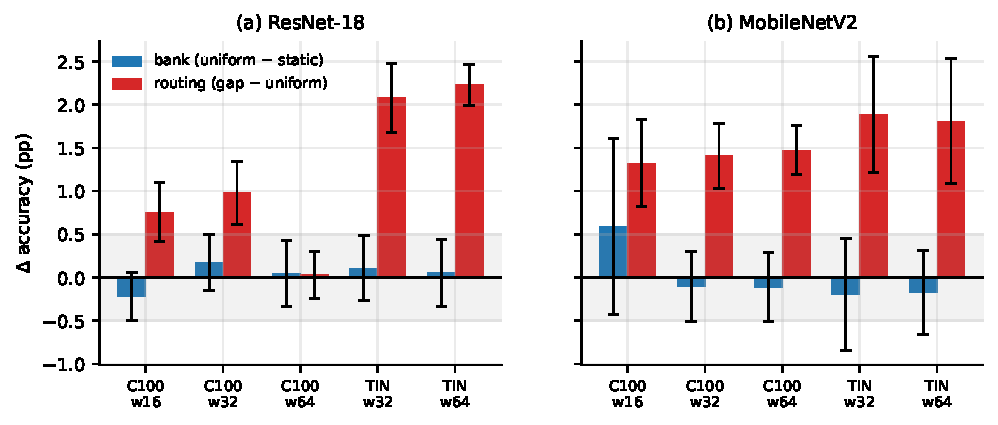
\includegraphics[width=\textwidth]{fig/g1_decomp_both.pdf}
\caption{Bank term ($\texttt{uniform}-\texttt{static}$) and routing term
($\texttt{gap}-\texttt{uniform}$) in the five conditions, for (a)
ResNet-18, (b) MobileNetV2 and (c) VGG-16, \SI{95}{\percent} CIs. The
shaded band is the $\pm$\SI{0.5}{pp} margin.}
\label{fig:mbdecomp}
\end{figure}

Figure~\ref{fig:mbdecomp} splits the total effect
$\texttt{gap}-\texttt{static}$ into the bank term and the routing term in
the five main conditions of each backbone (Tables~\ref{tab:decomp},
\ref{tab:mbdecomp} and~\ref{tab:vgdecomp}).

\paragraph{The bank term.} On ResNet-18 the bank term is equivalent to
zero in all five conditions, with $p_{\text{TOST}}$ between 0.014 and
0.025; the largest in magnitude is \V{bankCA}\,pp, at CIFAR-100 width 16.
On MobileNetV2 it is never significantly different from zero. It is
equivalent to zero on CIFAR-100 at widths 32 and 64
($p_{\text{TOST}}=\V{mbbankCBT}$ and \V{mbbankCCT}). At CIFAR-100 width 16
and at both Tiny-ImageNet widths it is inconclusive: the point estimates
are small (\V{mbbankCA}, \V{mbbankTA} and \V{mbbankTB}\,pp; the first lies
just outside the margin) and the confidence intervals extend beyond it, so
neither equivalence nor a difference is shown. At CIFAR-100 width 16 the
MobileNetV2 \texttt{static} arm itself is unusually variable across seeds
(Table~\ref{tab:mballruns}). On VGG-16 it is also never significantly
different from zero. It is equivalent to zero on CIFAR-100 at width 64 and
on Tiny-ImageNet at width 32 ($p_{\text{TOST}}=\V{vgbankCCT}$ and
\V{vgbankTAT}) and inconclusive in the other three conditions, where every
point estimate lies inside the margin (the largest in magnitude is
\V{vgbankmax}\,pp) but the confidence interval does not. Over the three
backbones the bank term is significant in none of the fifteen pairs and
equivalent to zero in \V{allbankeq}. On MobileNetV2 and VGG-16 static and
bank kernels share one initialisation, so their bank terms are free of
the initialisation mismatch that affects the ResNet-18 bank term
(Section~\ref{sec:threats}), and they give the same answer.

\paragraph{The routing term.} The routing term is positive with $p<0.05$
in \V{allrout} of the fifteen pairs: in \V{rbnrout} of five on ResNet-18,
in all five on MobileNetV2, where it ranges from \V{mbroutmin} to
\V{mbroutmax}\,pp, and in \V{vgnrout} of five on VGG-16. The VGG-16
exception is CIFAR-100 at width 32 (\V{vgroutCB}\,pp, $p=\V{vgroutCBp}$).
Because the bank term is never significant, the total effect
$\texttt{gap}-\texttt{static}$ is essentially the routing term: on
ResNet-18 at Tiny-ImageNet width 64, for example, routing is
\V{routTB}\,pp of a \V{effTB}\,pp total. Where the bank term is slightly
negative, as at ResNet-18 CIFAR-100 width 16 (the \V{bankCA}\,pp above),
the routing term exceeds the total, which is why we report no percentage
share. On VGG-16 at CIFAR-100 width 64 the same arithmetic produces a
significant routing term (\V{vgroutCC}\,pp, $p=\V{vgroutCCp}$) without a
total effect: the bank term is \V{vgbankCC}\,pp (equivalent to zero), and
the sum of the two, \V{vgeffCC}\,pp, is equivalent to zero as well
(Section~\ref{sec:null}).

\paragraph{Where the effect appears.} Dynamic convolution beats the plain
network in \V{alleff} of the fifteen pairs (Figure~\ref{fig:width}). On
MobileNetV2 the total effect is roughly flat across width on both
datasets, from \V{mbtotmin} to \V{mbtotmax}\,pp. On ResNet-18 it is
\V{effCA}\,pp at CIFAR-100 width 16 ($p\V{effCAp}$), \V{effCB}\,pp at width
32 ($p\V{effCBp}$) and \V{effCC}\,pp at width 64 ($p\V{effCCp}$), and
\V{effTA} and \V{effTB}\,pp on Tiny-ImageNet at widths 32 and 64. VGG-16
follows the ResNet-18 pattern: \V{vgeffCA}, \V{vgeffCB} and
\V{vgeffCC}\,pp on CIFAR-100 at widths 16, 32 and 64
($p=\V{vgeffCAp}$, \V{vgeffCBp} and \V{vgeffCCp}), and \V{vgeffTA} and
\V{vgeffTB}\,pp on Tiny-ImageNet. The two pairs without an effect, CIFAR-100
at width 64 on ResNet-18 and on VGG-16, are the subject of
Section~\ref{sec:null}. In \V{alleffrout} of the \V{alleff} pairs with an
effect the routing term is significant on its own; the remaining one is
the VGG-16 condition above. Figures~\ref{fig:sweep} and~\ref{fig:decomp}
in the appendix show the ResNet-18 accuracies and decomposition
separately.

\begin{table}[!htbp]\centering\small
\caption{ResNet-18: bank and routing terms, paired by seed. The bank
term is equivalent to zero in all five conditions.}
\label{tab:decomp}
\begin{tabular}{l r rll rl rl}
\toprule
& & \multicolumn{3}{c}{bank (\texttt{uniform}$-$\texttt{static})}
& \multicolumn{2}{c}{routing (\texttt{gap}$-$\texttt{uniform})}
& \multicolumn{2}{c}{total} \\
\cmidrule(lr){3-5}\cmidrule(lr){6-7}\cmidrule(lr){8-9}
dataset & width & $\Delta$ (pp) & $p_{\text{TOST}}$ & verdict & $\Delta$ (pp) & $p$ & $\Delta$ (pp) & $p$ \\
\midrule
CIFAR-100 & 16 & -0.223 & 0.0251 & equivalent & +0.755 & 0.0023 & +0.532 & 0.0023 \\
CIFAR-100 & 32 & +0.175 & 0.0242 & equivalent & +0.978 & 0.0010 & +1.153 & $<10^{-4}$ \\
CIFAR-100 & 64 & +0.048 & 0.0142 & equivalent & +0.032 & 0.7752 & +0.080 & 0.6158 \\
Tiny-ImageNet & 32 & +0.107 & 0.0218 & equivalent & +2.078 & $<10^{-4}$ & +2.185 & $<10^{-4}$ \\
Tiny-ImageNet & 64 & +0.053 & 0.0157 & equivalent & +2.228 & $<10^{-4}$ & +2.282 & $<10^{-4}$ \\
\bottomrule
\end{tabular}
\end{table}

\begin{table}[!htbp]\centering\small
\caption{MobileNetV2: bank and routing terms, paired by seed.}
\label{tab:mbdecomp}
\begin{tabular}{l r rll rl rl}
\toprule
& & \multicolumn{3}{c}{bank (\texttt{uniform}$-$\texttt{static})}
& \multicolumn{2}{c}{routing (\texttt{gap}$-$\texttt{uniform})}
& \multicolumn{2}{c}{total} \\
\cmidrule(lr){3-5}\cmidrule(lr){6-7}\cmidrule(lr){8-9}
dataset & width & $\Delta$ (pp) & $p_{\text{TOST}}$ & verdict & $\Delta$ (pp) & $p$ & $\Delta$ (pp) & $p$ \\
\midrule
CIFAR-100 & 16 & +0.593 & 0.5884 & inconclusive & +1.322 & 0.0011 & +1.915 & 0.0225 \\
CIFAR-100 & 32 & -0.102 & 0.0269 & equivalent & +1.408 & 0.0002 & +1.307 & 0.0015 \\
CIFAR-100 & 64 & -0.113 & 0.0275 & equivalent & +1.473 & $<10^{-4}$ & +1.360 & 0.0002 \\
Tiny-ImageNet & 32 & -0.193 & 0.1393 & inconclusive & +1.888 & 0.0008 & +1.695 & 0.0028 \\
Tiny-ImageNet & 64 & -0.175 & 0.0742 & inconclusive & +1.807 & 0.0014 & +1.632 & 0.0002 \\
\bottomrule
\end{tabular}
\end{table}

\begin{table}[!htbp]\centering\small
\caption{VGG-16: bank and routing terms, paired by seed.}
\label{tab:vgdecomp}
\begin{tabular}{l r rll rl rl}
\toprule
& & \multicolumn{3}{c}{bank (\texttt{uniform}$-$\texttt{static})}
& \multicolumn{2}{c}{routing (\texttt{gap}$-$\texttt{uniform})}
& \multicolumn{2}{c}{total} \\
\cmidrule(lr){3-5}\cmidrule(lr){6-7}\cmidrule(lr){8-9}
dataset & width & $\Delta$ (pp) & $p_{\text{TOST}}$ & verdict & $\Delta$ (pp) & $p$ & $\Delta$ (pp) & $p$ \\
\midrule
CIFAR-100 & 16 & +0.145 & 0.0621 & inconclusive & +0.718 & 0.0375 & +0.863 & 0.0020 \\
CIFAR-100 & 32 & -0.148 & 0.0834 & inconclusive & +0.627 & 0.0569 & +0.478 & 0.0077 \\
CIFAR-100 & 64 & -0.188 & 0.0147 & equivalent & +0.373 & 0.0025 & +0.185 & 0.0766 \\
Tiny-ImageNet & 32 & +0.128 & 0.0039 & equivalent & +1.637 & 0.0001 & +1.765 & $<10^{-4}$ \\
Tiny-ImageNet & 64 & +0.250 & 0.1458 & inconclusive & +1.230 & 0.0055 & +1.480 & 0.0023 \\
\bottomrule
\end{tabular}
\end{table}

\begin{figure}[!htbp]\centering
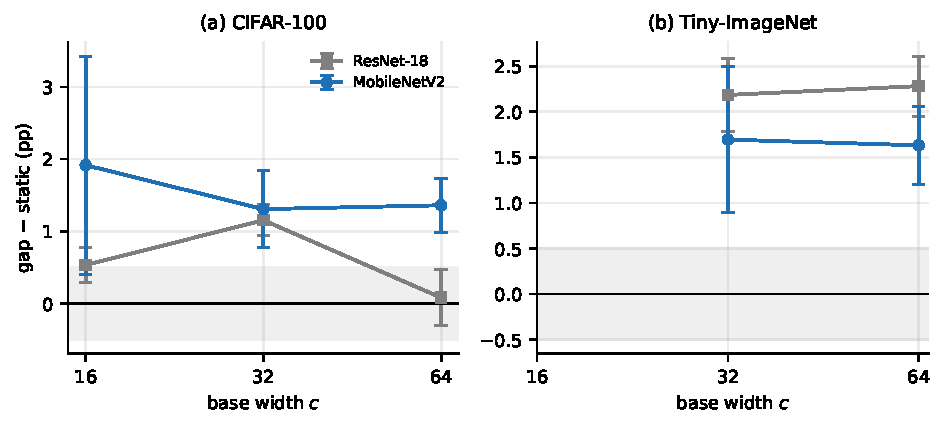
\includegraphics[width=\textwidth]{fig/g3_width_both.pdf}
\caption{$\texttt{gap}-\texttt{static}$ against width for the three
backbones, \SI{95}{\percent} CIs. ResNet-18 and VGG-16 have a null on
CIFAR-100 at width 64; MobileNetV2 does not.}
\label{fig:width}
\end{figure}

\section{The null: CIFAR-100 at width 64 on ResNet-18 and VGG-16}\label{sec:null}

\begin{figure}[!htbp]\centering
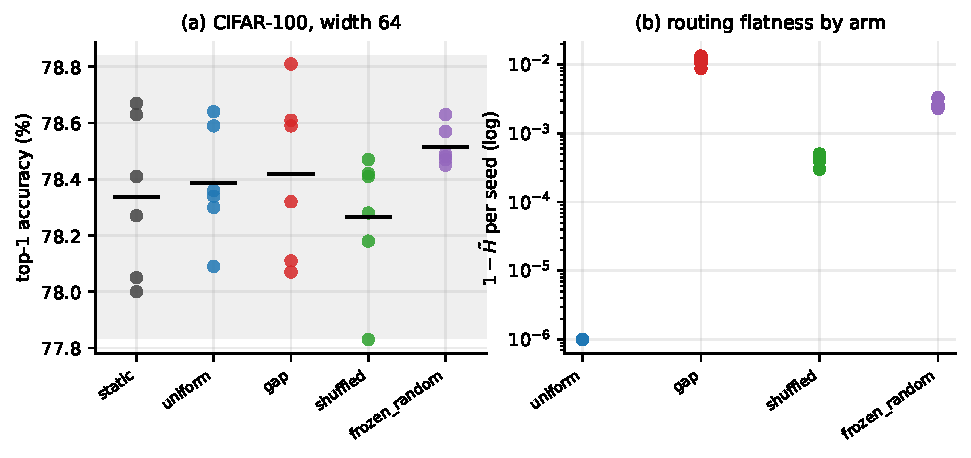
\includegraphics[width=\textwidth]{fig/f3_w64.pdf}
\caption{ResNet-18, CIFAR-100, width 64. (a) Every run of the five arms; bars are
arm means and the shaded band is $\pm$\SI{0.5}{pp} around
\texttt{static}. (b) Router flatness $1-\tilde H$ per seed, log scale;
\texttt{uniform} is exactly zero and is drawn at the axis floor.}
\label{fig:w64}
\end{figure}

On ResNet-18 at CIFAR-100 width 64 every arm is equivalent to the plain
network (Table~\ref{tab:vsstatic}, Figure~\ref{fig:w64}). The largest gap
between arm means is \V{spread64}\,pp, against a median within-arm seed
standard deviation of \V{seedsd64}\,pp, and a one-way ANOVA across the five
arms gives $F(4,25)=\V{anovaF}$, $p=\V{anovaP}$. The null is not a power
artefact: the minimum detectable routing term is \V{mde}\,pp
(Section~\ref{sec:stats}). On MobileNetV2 the same condition behaves like
every other: the five arms differ ($F=\V{mbanovaF}$, $p\V{mbanovaP}$) and
$\texttt{gap}-\texttt{static}$ is \V{mbeffCC}\,pp (\SI{95}{\percent} CI
[\V{mbeffCClo}, \V{mbeffCChi}], $p=\V{mbeffCCp}$).

VGG-16 reproduces the ResNet-18 null (Table~\ref{tab:mbw64}). No arm beats
the plain network: $\texttt{gap}-\texttt{static}$ is \V{vgeffCC}\,pp
(\SI{95}{\percent} CI [\V{vgeffCClo}, \V{vgeffCChi}],
$p_{\text{TOST}}=\V{vgeffCCT}$, equivalent), \texttt{uniform} and
\texttt{frozen\_random} are equivalent to it as well, and
\texttt{shuffled} is inconclusive (\V{vgwshuffledstatic}\,pp). Unlike on
ResNet-18 the five VGG-16 arms are not all alike ($F(4,25)=\V{vganovaF}$,
$p=\V{vganovaP}$; largest gap between arm means \V{vgspread64}\,pp): the
trained router lies above the constant mixture and above the shuffled
router (Section~\ref{sec:router}), but not above the plain network. The
two backbones with the null are the two in which nearly every parameter
sits in a full dynamic convolution; VGG-16 has no residual connections,
so the null does not depend on them. We tested two explanations of the
null, both on ResNet-18 first.

\subsection{Saturation: a recorded prediction that failed}

The saturation account says the routing effect vanishes once a network
memorises its training data. On CIFAR-100 the ResNet-18 null coincides
with the lowest static training loss, \V{lossCC}.

\paragraph{Tiny-ImageNet, width 32.} Here $\texttt{gap}-\texttt{static}$
is \V{effTA}\,pp (\SI{95}{\percent} CI [\V{effTAlo}, \V{effTAhi}],
$p\V{effTAp}$), against \V{effCB}\,pp on CIFAR-100 at the same width.
Before these runs we expected the effect to be larger than on CIFAR-100,
since the static arm trains to a higher loss (\V{lossTA} against
\V{lossCB}). That expectation held, but it was stated and not recorded,
it predicted only a direction, and we do not treat it as evidence.

\paragraph{Tiny-ImageNet, width 64.} Before these runs we recorded, in
writing and dated, the prediction in Table~\ref{tab:predict}: the static
arm would train to a loss below 0.05, and the effect would then fall below
\SI{0.5}{pp} and be equivalent to zero. The loss condition held
(\V{lossTB}) and the effect did not vanish:
$\texttt{gap}-\texttt{static}=\V{effTB}$\,pp, \SI{95}{\percent} CI
[\V{effTBlo}, \V{effTBhi}], $p=\V{predP}$ (Figure~\ref{fig:tin}). The
prediction failed.

\begin{figure}[!htbp]\centering
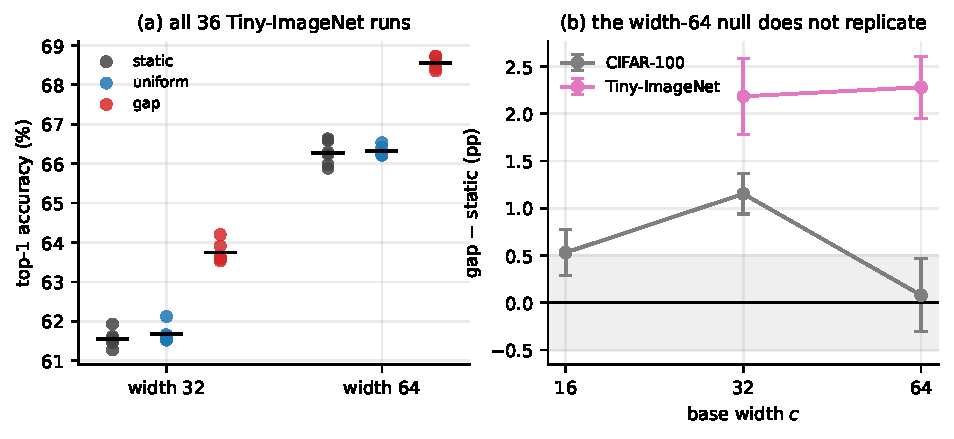
\includegraphics[width=\textwidth]{fig/f7_tin.pdf}
\caption{ResNet-18. (a) All 36 Tiny-ImageNet runs. (b) $\texttt{gap}-\texttt{static}$
by width on both datasets, \SI{95}{\percent} CIs. The CIFAR-100
width-64 null does not appear on Tiny-ImageNet.}
\label{fig:tin}
\end{figure}

\begin{table}[!htbp]\centering\small
\caption{ResNet-18: the prediction recorded before the Tiny-ImageNet width-64 runs,
and the outcome. Both conditions were stated as required.}
\label{tab:predict}
\begin{tabular}{l p{5.4cm} p{4.6cm} l}
\toprule
& prediction & measured & outcome \\
\midrule
(a) & \texttt{gap} $-$ \texttt{static} below \SI{0.5}{pp}, equivalent by TOST & +2.282 pp, $p=1.0\times10^{-5}$, $p_{\text{TOST}}=1.0000$ & failed \\
(b) & static final training loss below 0.05 & 0.021 & held \\
\bottomrule
\end{tabular}
\end{table}

\paragraph{Training loss does not order the effect.} Ordered by the
static arm's final training loss (Table~\ref{tab:satur},
Figure~\ref{fig:pred}b), the ResNet-18 effects do not follow:
Tiny-ImageNet at width 64 trains to a loss close to CIFAR-100 at width 32
and shows twice the effect, and CIFAR-100 at width 16 trains to the
highest loss and shows one of the smallest. MobileNetV2 is consistent
with the saturation account but cannot rescue it
(Figure~\ref{fig:losseffect}): none of its static arms trains below
\V{mblossCC} under this recipe, and every MobileNetV2 condition has an
effect. VGG-16 repeats the ResNet-18 pattern without a recorded
prediction: its null coincides with its lowest static training loss
(\V{vglossCC}), but on Tiny-ImageNet at width 64 the static arm trains to
\V{vglossTB}, below the \V{vglossCB} of CIFAR-100 at width 32, and the
effect there is \V{vgeffTB}\,pp against \V{vgeffCB}\,pp. The Tiny-ImageNet
width-64 points of ResNet-18 and VGG-16, each at a low loss with a clear
effect, rule out a single loss threshold for all fifteen points, and a
threshold chosen after seeing them would not be evidence. We do not adopt
it.

\begin{figure}[!htbp]\centering
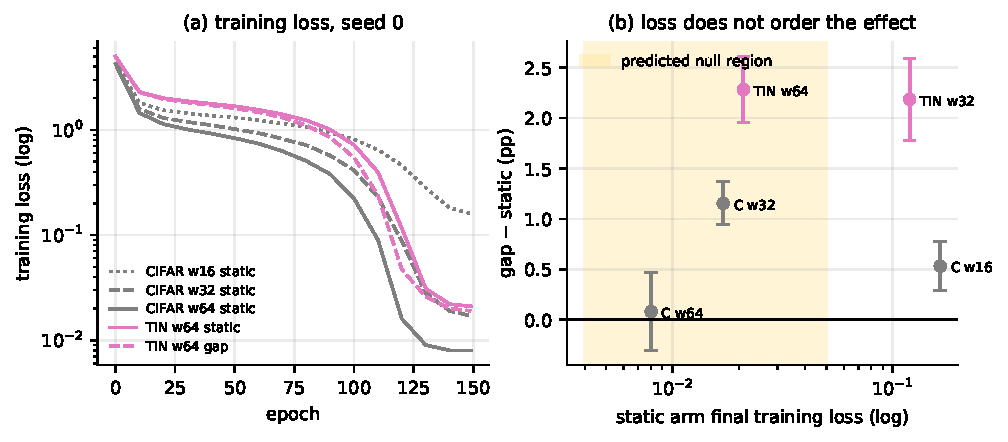
\includegraphics[width=\textwidth]{fig/f8_prediction.pdf}
\caption{ResNet-18. (a) Training loss of static and gap arms, seed 0, log scale.
(b) Routing effect against the final training loss of the static arm in
all five conditions. The shaded band is the region the prediction
associated with a null.}
\label{fig:pred}
\end{figure}

\begin{table}[!htbp]\centering\small
\caption{ResNet-18: five conditions ordered by the final training loss of the
static arm.}
\label{tab:satur}
\begin{tabular}{l r r rl l}
\toprule
dataset & width & static train loss & $\texttt{gap}-\texttt{static}$ (pp) & \SI{95}{\percent} CI & verdict \\
\midrule
CIFAR-100 & 64 & 0.0080 & +0.080 & [-0.305, +0.465] & equivalent \\
CIFAR-100 & 32 & 0.0170 & +1.153 & [+0.940, +1.367] & higher \\
Tiny-ImageNet & 64 & 0.0210 & +2.282 & [+1.952, +2.611] & higher \\
Tiny-ImageNet & 32 & 0.1194 & +2.185 & [+1.781, +2.589] & higher \\
CIFAR-100 & 16 & 0.1643 & +0.532 & [+0.292, +0.771] & higher \\
\bottomrule
\end{tabular}
\end{table}

\begin{figure}[!htbp]\centering
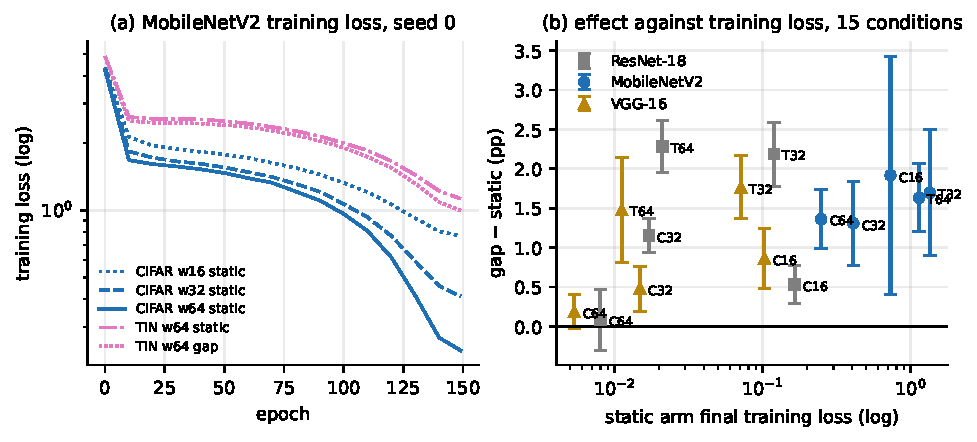
\includegraphics[width=\textwidth]{fig/g6_loss_effect.pdf}
\caption{(a) MobileNetV2 training loss, seed 0, log scale. (b)
$\texttt{gap}-\texttt{static}$ against the static arm's final training
loss for the three backbones and all five conditions, \SI{95}{\percent}
CIs.}
\label{fig:losseffect}
\end{figure}

\subsection{Temperature: the null survives annealing}

With $\tau=1$ the bank could be undertrained, in which case the null
would say nothing about dynamic convolution. Repeating \texttt{gap} with
the annealed schedule leaves it in place: annealed \texttt{gap} against
\texttt{static} is \V{ansC}\,pp with $p_{\text{TOST}}=\V{ansCT}$, a
tighter equivalence than the \V{constT64} at $\tau=1$
(Section~\ref{sec:temp}). On VGG-16 the same holds: annealed \texttt{gap}
against \texttt{static} is \V{vgansC}\,pp with
$p_{\text{TOST}}=\V{vgansCT}$.

\paragraph{What remains.} On ResNet-18 and VGG-16, on CIFAR-100, at
width 64, dynamic convolution has no effect over the plain network; the
result is well powered on ResNet-18, is a positive equivalence on both,
holds under both schedules, and does not appear on Tiny-ImageNet or on
MobileNetV2. Training loss does not explain it, temperature does not cause
it and residual connections are not needed for it. Between the conditions,
input resolution, final feature-map size and number of classes differ;
between the backbones, the share of parameters in dynamic layers and full
against depthwise convolution differ. None was isolated here, and the null
remains unexplained.

\section{Does the router need to be trained?}\label{sec:router}

\begin{figure}[!htbp]\centering
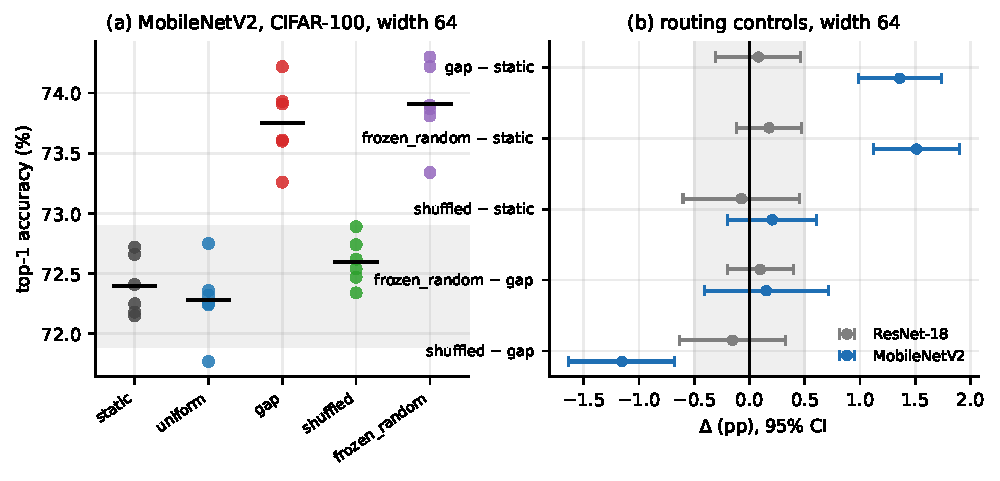
\includegraphics[width=\textwidth]{fig/g2_mb_w64.pdf}
\caption{CIFAR-100, width 64. (a) Every MobileNetV2 run of the five arms;
bars are arm means, the band is $\pm$\SI{0.5}{pp} around \texttt{static}.
(b) The routing controls on the three backbones, \SI{95}{\percent}
CIs.}
\label{fig:mbw64}
\end{figure}

The controls \texttt{shuffled} and \texttt{frozen\_random} were run on
CIFAR-100 at width 64 on every backbone (Table~\ref{tab:mbw64},
Figure~\ref{fig:mbw64}). They can only answer this question where routing
has an effect to explain: against the plain network on MobileNetV2, and
against the constant mixture on VGG-16.

\paragraph{MobileNetV2.} A router frozen at its random initialisation
beats \texttt{static} by \V{mbwfrozenrandomstatic}\,pp and \texttt{uniform}
by \V{mbwfrozenrandomuniform}\,pp ($p=\V{mbwfrozenrandomuniformp}$), and is
not distinguishable from the trained router
($\texttt{frozen\_random}-\texttt{gap}=\V{mbwfrozenrandomgap}$\,pp,
\SI{95}{\percent} CI [\V{mbwfrozenrandomgaplo}, \V{mbwfrozenrandomgaphi}],
$p=\V{mbwfrozenrandomgapp}$). It is not equivalent to it at our margin
either ($p_{\text{TOST}}=\V{mbwfrozenrandomgapT}$), so the claim is that no
difference was detected, not that none exists. Routing each image with
another image's descriptor removes the benefit: \texttt{shuffled} is not
distinguishable from \texttt{static} (\V{mbwshuffledstatic}\,pp,
$p=\V{mbwshuffledstaticp}$) and is lower than \texttt{gap}
(\V{mbwshuffledgap}\,pp, $p=\V{mbwshuffledgapp}$). Read together, the
benefit on MobileNetV2 requires that each image's own descriptor determine
its mixture, and does not require the router to be trained: a fixed random
map from descriptors to mixtures was enough. That map is a single random
draw shared by all six seeds, so the result does not show that any random
router would do. The frozen router's weights are
held as buffers and are not trained, so the gain is not a product of the
\V{mbrouterK}K trainable router parameters either.

\paragraph{VGG-16.} Here no arm beats the plain network
(Section~\ref{sec:null}), but the trained router beats the constant
mixture: $\texttt{gap}-\texttt{uniform}=\V{vgwgapuniform}$\,pp
(\SI{95}{\percent} CI [\V{vgwgapuniformlo}, \V{vgwgapuniformhi}],
$p=\V{vgwgapuniformp}$). The frozen router does not: it is equivalent to
the constant mixture ($\V{vgwfrozenrandomuniform}$\,pp,
$p_{\text{TOST}}=\V{vgwfrozenrandomuniformT}$), and the direct comparison
with the trained router is inconclusive
($\texttt{frozen\_random}-\texttt{gap}=\V{vgwfrozenrandomgap}$\,pp,
\SI{95}{\percent} CI [\V{vgwfrozenrandomgaplo},
\V{vgwfrozenrandomgaphi}], $p=\V{vgwfrozenrandomgapp}$). The shuffled
router is lower than the trained one (\V{vgwshuffledgap}\,pp,
$p=\V{vgwshuffledgapp}$). On VGG-16, then, only the trained router is
distinguishable from the constant mixture, whereas on MobileNetV2 the
frozen router is as well; the direct comparison of frozen and trained
router is inconclusive on both. The effect involved on VGG-16 is small: \V{vgwgapuniform}\,pp over a constant
mixture whose own difference from the plain network is \V{vgbankCC}\,pp.

\paragraph{ResNet-18.} In the same condition every ResNet-18 arm,
including both controls, is equivalent to the plain network, and
$\texttt{frozen\_random}-\texttt{gap}$ is \V{frzVgap}\,pp
($p_{\text{TOST}}=\V{frzVgapT}$). With no benefit over either the plain
network or the constant mixture to explain, this says nothing about
whether routing needs to be trained.

\paragraph{Summary.} Whether the router has to be trained depends on the
backbone: on MobileNetV2 a frozen random router does as well as a trained
one; on VGG-16 only the trained router departs from the constant mixture;
on ResNet-18 the question cannot be tested. All of this rests on one condition, CIFAR-100 at width 64, and
on one random draw of the frozen router.

\paragraph{What the routers output.} The trained router is the furthest
from uniform on ResNet-18 and MobileNetV2 (Table~\ref{tab:mbentw64}; the
measurement is described in Section~\ref{sec:entdef}). On MobileNetV2 the
frozen router is \V{mbeFrzRatio} times closer to uniform
($1-\tilde H=\V{mbeFrz}$ against \V{mbeGap}), but its departure is spread
over the network: its entropy reaches 0.9999 in only \V{mbeFrzFlat} of the
\V{mbnlayers} dynamic layers. The \texttt{shuffled} router, whose input
carries no information about the image it routes, trains itself to
near-uniform on both ($1-\tilde H=\V{mbeShuf}$ on MobileNetV2,
\V{rbeShuf} on ResNet-18). On ResNet-18 the trained router's entropy is
below that of the controls (Figure~\ref{fig:w64}b), so it is further from
uniform. Entropy alone does not show whether the mixture varies with the
input, since a constant mixture that is not uniform would also have low
entropy; at this width, whatever the router does changes no accuracy. The
VGG-16 entropies are in its result files, which were not available for
this draft.

\begin{table}[!htbp]\centering\small
\caption{Routing controls on CIFAR-100 at width 64, three backbones,
paired by seed.}
\label{tab:mbw64}
\resizebox{\textwidth}{!}{%
\begin{tabular}{l rll rll rll}
\toprule
& \multicolumn{3}{c}{ResNet-18} & \multicolumn{3}{c}{MobileNetV2} & \multicolumn{3}{c}{VGG-16} \\
\cmidrule(lr){2-4}\cmidrule(lr){5-7}\cmidrule(lr){8-10}
comparison & $\Delta$ (pp) & $p$ & verdict & $\Delta$ (pp) & $p$ & verdict & $\Delta$ (pp) & $p$ & verdict \\
\midrule
\texttt{uniform} $-$ \texttt{static} & +0.048 & 0.7573 & equivalent & -0.113 & 0.4978 & equivalent & -0.188 & 0.1273 & equivalent \\
\texttt{gap} $-$ \texttt{static} & +0.080 & 0.6158 & equivalent & +1.360 & 0.0002 & higher & +0.185 & 0.0766 & equivalent \\
\texttt{shuffled} $-$ \texttt{static} & -0.073 & 0.7361 & equivalent & +0.205 & 0.2456 & inconclusive & -0.233 & 0.1896 & inconclusive \\
\texttt{frozen\_random} $-$ \texttt{static} & +0.177 & 0.1874 & equivalent & +1.512 & 0.0002 & higher & -0.095 & 0.5183 & equivalent \\
\texttt{frozen\_random} $-$ \texttt{gap} & +0.097 & 0.4433 & equivalent & +0.152 & 0.5196 & inconclusive & -0.280 & 0.0743 & inconclusive \\
\texttt{shuffled} $-$ \texttt{gap} & -0.153 & 0.4507 & inconclusive & -1.155 & 0.0016 & lower & -0.418 & 0.0257 & lower \\
\texttt{frozen\_random} $-$ \texttt{uniform} & +0.128 & 0.2605 & equivalent & +1.625 & 0.0008 & higher & +0.093 & 0.3111 & equivalent \\
\texttt{gap} $-$ \texttt{uniform} & +0.032 & 0.7752 & equivalent & +1.473 & $<10^{-4}$ & higher & +0.373 & 0.0025 & higher \\
\bottomrule
\end{tabular}}
\end{table}

\begin{table}[!htbp]\centering\small
\caption{Routing entropy by arm, CIFAR-100 width 64, per-seed means over
the recorded images and layers. Flat layers: the number of the
\V{mbnlayers} MobileNetV2 dynamic layers with $\tilde H\ge0.9999$, range
over seeds.}
\label{tab:mbentw64}
\begin{tabular}{l rr rrrr r}
\toprule
& \multicolumn{2}{c}{ResNet-18} & \multicolumn{5}{c}{MobileNetV2} \\
\cmidrule(lr){2-3}\cmidrule(lr){4-8}
arm & mean $\tilde H$ & $1-\tilde H$ & mean $\tilde H$ & min & max & $1-\tilde H$ & flat layers \\
\midrule
\texttt{uniform} & 1.0000 & 0.00000 & 1.00000 & 1.00000 & 1.00000 & 0.00000 & 17 \\
\texttt{gap} & 0.9885 & 0.01147 & 0.98680 & 0.98272 & 0.98955 & 0.01320 & 2--4 \\
\texttt{frozen\_random} & 0.9971 & 0.00287 & 0.99706 & 0.99649 & 0.99736 & 0.00294 & 0--2 \\
\texttt{shuffled} & 0.9996 & 0.00040 & 0.99995 & 0.99992 & 0.99996 & 0.00005 & 14--16 \\
\bottomrule
\end{tabular}
\end{table}

\section{Bank size}\label{sec:ksize}

\begin{figure}[!htbp]\centering
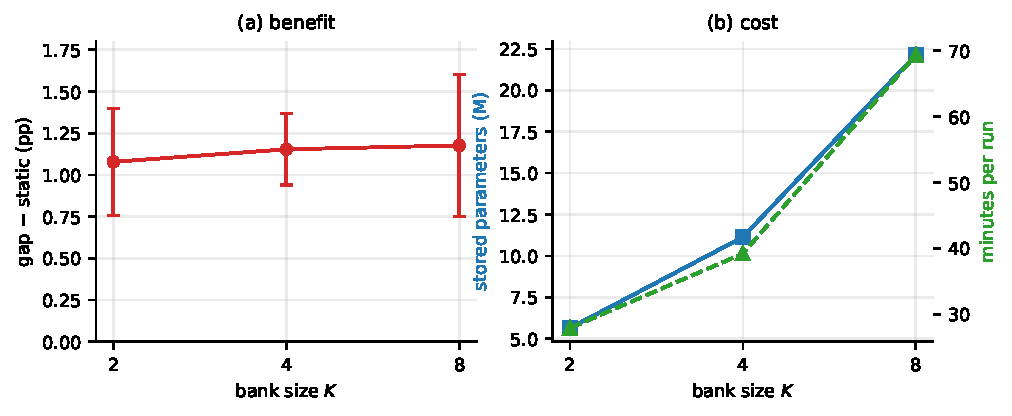
\includegraphics[width=0.84\textwidth]{fig/f6_k.pdf}
\caption{ResNet-18, CIFAR-100, width 32. (a) Effect over \texttt{static} for
$K\in\{2,4,8\}$, \SI{95}{\percent} CIs. (b) Stored parameters and
training time.}
\label{fig:k}
\end{figure}

At CIFAR-100 width 32 all three bank sizes beat \texttt{static} on
ResNet-18 and MobileNetV2 (Tables~\ref{tab:k} and~\ref{tab:mbk},
Figure~\ref{fig:mbtemp}b); on VGG-16 $K=4$ and $K=8$ do and $K=2$ is not
distinguishable from \texttt{static} (\V{vgk2s}\,pp, $p=\V{vgk2sp}$;
Table~\ref{tab:vgk}). On ResNet-18 no pair of sizes is distinguishable and
every pair is equivalent (Table~\ref{tab:kpairs}): $K=8$ over $K=2$ is
\V{k82}\,pp ($p=\V{k82p}$). Going from $K=2$ to $K=8$ multiplies stored
parameters by \V{kpar} and training time by \V{ktime} (Figure~\ref{fig:k}).
On MobileNetV2 $K=8$ over $K=2$ is \V{mbk82}\,pp ($p=\V{mbk82p}$) and on
VGG-16 \V{vgk82}\,pp ($p=\V{vgk82p}$): not distinguishable, but not
equivalent at our margin either. On all three backbones, then, nothing
beyond $K=2$ was detected.

\begin{table}[!htbp]\centering\small
\caption{ResNet-18: bank size at CIFAR-100 width 32. Differences are against the
\texttt{static} row.}
\label{tab:k}
\begin{tabular}{l rr rl l rr}
\toprule
$K$ & accuracy & sd & $\Delta$ (pp) & \SI{95}{\percent} CI & $p$ & params (M) & min/run \\
\midrule
2 & 75.950 & 0.148 & +1.078 & [+0.758, +1.399] & 0.0003 & 5.64 & 27.9 \\
4 & 76.025 & 0.156 & +1.153 & [+0.940, +1.367] & $<10^{-4}$ & 11.13 & 39.2 \\
8 & 76.048 & 0.242 & +1.177 & [+0.749, +1.604] & 0.0009 & 22.12 & 69.3 \\
\midrule \texttt{static} & 74.872 & 0.262 & -- & -- & -- & 2.82 & 8.6 \\
\bottomrule
\end{tabular}
\end{table}

\begin{table}[!htbp]\centering\small
\caption{ResNet-18: pairwise comparisons between bank sizes, CIFAR-100
width 32.}
\label{tab:kpairs}
\begin{tabular}{l rl ll l}
\toprule
comparison & $\Delta$ (pp) & \SI{95}{\percent} CI & $p$ & $p_{\text{TOST}}$ & verdict \\
\midrule
$K=4$ vs $K=2$ & +0.075 & [-0.087, +0.237] & 0.2878 & 0.0005 & equivalent \\
$K=8$ vs $K=4$ & +0.023 & [-0.286, +0.332] & 0.8538 & 0.0053 & equivalent \\
$K=8$ vs $K=2$ & +0.098 & [-0.182, +0.379] & 0.4091 & 0.0072 & equivalent \\
\bottomrule
\end{tabular}
\end{table}

\begin{table}[!htbp]\centering\small
\caption{MobileNetV2: bank size at CIFAR-100 width 32.}
\label{tab:mbk}
\begin{tabular}{l rr rl l rr}
\toprule
$K$ & accuracy & sd & $\Delta$ (pp) & \SI{95}{\percent} CI & $p$ & params (M) & min/run \\
\midrule
2 & 71.773 & 0.490 & +0.998 & [+0.487, +1.510] & 0.0041 & 1.14 & 51.6 \\
4 & 72.082 & 0.356 & +1.307 & [+0.771, +1.843] & 0.0015 & 1.20 & 47.3 \\
8 & 71.885 & 0.400 & +1.110 & [+0.647, +1.573] & 0.0016 & 1.34 & 98.8 \\
\midrule \texttt{static} & 70.775 & 0.217 & -- & -- & -- & 0.82 & 18.0 \\
\bottomrule
\end{tabular}
\end{table}

\begin{table}[!htbp]\centering\small
\caption{VGG-16: bank size at CIFAR-100 width 32.}
\label{tab:vgk}
\begin{tabular}{l rr rl l rr}
\toprule
$K$ & accuracy & sd & $\Delta$ (pp) & \SI{95}{\percent} CI & $p$ & params (M) & min/run \\
\midrule
2 & 71.577 & 0.355 & +0.258 & [-0.313, +0.830] & 0.2978 & 7.48 & 19.9 \\
4 & 71.797 & 0.303 & +0.478 & [+0.193, +0.764] & 0.0077 & 14.84 & 26.0 \\
8 & 71.773 & 0.224 & +0.455 & [+0.113, +0.797] & 0.0189 & 29.55 & 40.9 \\
\midrule \texttt{static} & 71.318 & 0.228 & -- & -- & -- & 3.71 & 6.9 \\
\bottomrule
\end{tabular}
\end{table}

\section{Is routing worth its cost?}\label{sec:cost}

The answer depends on what is held fixed.

\subsection{Twice the width: equal parameters on ResNet-18 and VGG-16}\label{sec:matched}

\begin{figure}[!htbp]\centering
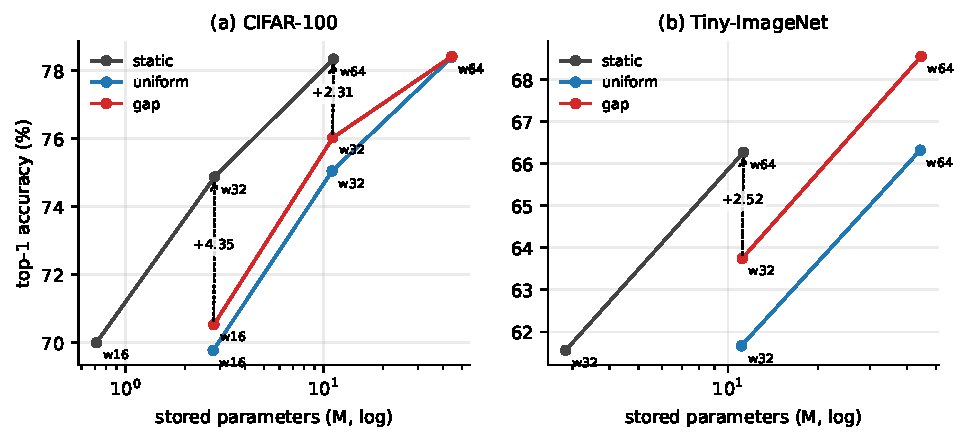
\includegraphics[width=\textwidth]{fig/f5_matched.pdf}
\caption{ResNet-18: accuracy against stored parameters. Dotted arrows join routed
and plain networks matched to within \SI{1}{\percent} on parameter
count.}
\label{fig:matched}
\end{figure}

On ResNet-18 the widths differ by a factor of two and the bank multiplies
convolution parameters by four, so a routed network at one width stores
almost exactly as many parameters as a plain network at the next width
up. That gives three matched comparisons without any extra runs
(Table~\ref{tab:matched}, Figure~\ref{fig:matched}). The plain network
wins all three: by \V{mMA}\,pp at 2.8M parameters and \V{mMB}\,pp at 11.2M
on CIFAR-100, and by \V{mMC}\,pp at 11.2M on Tiny-ImageNet. It also trains
faster in each case; on Tiny-ImageNet, \V{tMCs}\,min per run against
\V{tMCg}\,min. A fourth, unmatched comparison points the same way: the
$K=8$ network at width 32 stores 22.1M parameters, twice the plain
width-64 network, and trails it by \V{k8vs64}\,pp.

VGG-16 has the same arithmetic, since nearly all of its parameters are in
dynamic layers: the parameter ratio is \V{vgmMAr} in all three pairs
(Table~\ref{tab:vgmatched}). The plain network wins all three as well, by
\V{vgmMA} and \V{vgmMB}\,pp on CIFAR-100 and \V{vgmMC}\,pp on
Tiny-ImageNet ($p$\,\V{vgmMAp} in each).

On MobileNetV2 the same pairs are not matched: so few parameters sit in
dynamic layers that the routed network has only \V{mbmMBr} to \V{mbmMAr}
times the parameters of the plain network at twice its width
(Table~\ref{tab:mbmatched}, Figure~\ref{fig:mbmatched}). Even so, the
plain network wins only at the smallest width (\V{mbmMA}\,pp,
$p=\V{mbmMAp}$). On CIFAR-100 at width 32 and on Tiny-ImageNet the two are
not distinguishable (\V{mbmMB}\,pp, $p=\V{mbmMBp}$; \V{mbmMC}\,pp,
$p=\V{mbmMCp}$). Interpolating the static accuracy curve in
log-parameters to the routed network's parameter count puts the routed
network ahead in all three cases (static minus routed: \V{mbmMAi},
\V{mbmMBi} and \V{mbmMCi}\,pp); that comparison is an interpolation and has
no confidence interval.

\begin{table}[!htbp]\centering\small
\caption{ResNet-18: routed against plain networks at matched parameter counts,
paired by seed. Minutes are routed / plain per run. The last column is
the routed network's stored parameters divided by the plain one's; a pair
is called matched only within 10\,\%.}
\label{tab:matched}
\resizebox{\textwidth}{!}{%
\begin{tabular}{l l l rr rl l r l}
\toprule
dataset & routed & plain & routed & plain & $\Delta$ (pp) & \SI{95}{\percent} CI & $p$ & min/run & param ratio \\
\midrule
CIFAR-100 & \texttt{gap} w16 (2.79M) & \texttt{static} w32 (2.82M) & 70.527 & 74.872 & +4.345 & [+4.103, +4.587] & $<10^{-4}$ & 33.7 / 8.6 & 0.99 (matched) \\
CIFAR-100 & \texttt{gap} w32 (11.13M) & \texttt{static} w64 (11.22M) & 76.025 & 78.338 & +2.313 & [+1.870, +2.757] & $<10^{-4}$ & 39.2 / 18.8 & 0.99 (matched) \\
Tiny-ImageNet & \texttt{gap} w32 (11.16M) & \texttt{static} w64 (11.27M) & 63.745 & 66.265 & +2.520 & [+2.311, +2.729] & $<10^{-4}$ & 284.2 / 129.0 & 0.99 (matched) \\
\bottomrule
\end{tabular}}
\end{table}

\begin{table}[!htbp]\centering\small
\caption{VGG-16: \texttt{gap} at width $c$ against \texttt{static} at
width $2c$, paired by seed. $\Delta$ is plain minus routed; the ratio is
the routed network's stored parameters over the plain one's.}
\label{tab:vgmatched}
\resizebox{\textwidth}{!}{%
\begin{tabular}{l l l rr rl l l r}
\toprule
dataset & routed & plain & routed & plain & $\Delta$ (pp) & \SI{95}{\percent} CI & $p$ & verdict & ratio \\
\midrule
CIFAR-100 & \texttt{gap} w16 (3.72M) & \texttt{static} w32 (3.71M) & 66.082 & 71.318 & +5.237 & [+4.826, +5.648] & $<10^{-4}$ & higher & 1.00 \\
CIFAR-100 & \texttt{gap} w32 (14.84M) & \texttt{static} w64 (14.77M) & 71.797 & 74.807 & +3.010 & [+2.740, +3.280] & $<10^{-4}$ & higher & 1.00 \\
Tiny-ImageNet & \texttt{gap} w32 (14.86M) & \texttt{static} w64 (14.82M) & 60.813 & 63.300 & +2.487 & [+1.936, +3.037] & $<10^{-4}$ & higher & 1.00 \\
\bottomrule
\end{tabular}}
\end{table}

\begin{figure}[!htbp]\centering
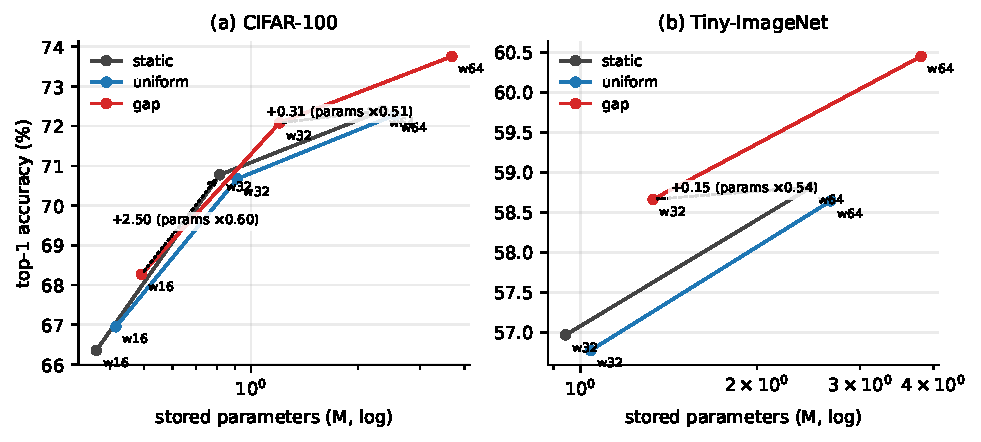
\includegraphics[width=\textwidth]{fig/g4_mb_matched.pdf}
\caption{MobileNetV2: accuracy against stored parameters. Arrows join
\texttt{gap} at width $c$ to \texttt{static} at width $2c$; labels give
the accuracy difference and the parameter ratio.}
\label{fig:mbmatched}
\end{figure}

\begin{table}[!htbp]\centering\small
\caption{MobileNetV2: \texttt{gap} at width $c$ against \texttt{static} at
width $2c$, paired by seed. $\Delta$ is plain minus routed. The ratio is
the routed network's stored parameters over the plain one's; none of
these pairs is matched. The last column compares \texttt{gap} with the
static curve interpolated to its parameter count.}
\label{tab:mbmatched}
\resizebox{\textwidth}{!}{%
\begin{tabular}{l l l rr rl l l r r}
\toprule
dataset & routed & plain & routed & plain & $\Delta$ (pp) & \SI{95}{\percent} CI & $p$ & verdict & ratio & $\Delta$ equal params \\
\midrule
CIFAR-100 & \texttt{gap} w16 (0.49M) & \texttt{static} w32 (0.82M) & 68.272 & 70.775 & +2.503 & [+1.927, +3.080] & 0.0001 & higher & 0.60 & -0.298 \\
CIFAR-100 & \texttt{gap} w32 (1.20M) & \texttt{static} w64 (2.35M) & 72.082 & 72.395 & +0.313 & [-0.103, +0.730] & 0.1111 & inconclusive & 0.51 & -0.713 \\
Tiny-ImageNet & \texttt{gap} w32 (1.33M) & \texttt{static} w64 (2.48M) & 58.662 & 58.817 & +0.155 & [-0.520, +0.830] & 0.5806 & inconclusive & 0.54 & -1.037 \\
\bottomrule
\end{tabular}}
\end{table}

\subsection{Equal compute}

Dynamic convolution is usually advertised at equal compute, and there the
picture is different (Table~\ref{tab:cost}). Doubling the width costs
roughly three to four times the multiply-accumulates of the routed network;
routing at the same width costs at most \V{rbmacextra}\,\% more on
ResNet-18, \V{mbmacextra}\,\% more on MobileNetV2 and \V{vgmacextra}\,\%
more on VGG-16, counted for an implementation that aggregates the kernel
per sample (on VGG-16 the per-sample mixing of large kernels at small
feature maps is a larger share of the cost). At the same width, routing
beats the plain network in \V{rbeqmac} of five conditions on ResNet-18,
\V{mbeqmac} on MobileNetV2 and \V{vgeqmac} on VGG-16. Our training
implementation computes $K$ convolutions per dynamic layer and is slower in
wall-clock time than either count suggests (Tables~\ref{tab:config},
\ref{tab:mbconfig} and~\ref{tab:vgconfig}); that is a property of the
implementation, not of the layer.

\paragraph{Summary.} Against a plain network of twice the width, routing
loses in all six pairs on ResNet-18 and VGG-16, where the two have the same
number of parameters, and in one of three on MobileNetV2, where the plain
network has \V{mbpinvlo} to \V{mbpinvhi} times the parameters. At equal
width routing beats the plain network in \V{alleff} of fifteen conditions.
Whether dynamic convolution is worth its cost therefore depends on the
cost held fixed and on the backbone.

\begin{table}[!htbp]\centering\small
\caption{The routed network under two cost views. Left: \texttt{static}
at width $2c$ minus \texttt{gap} at width $c$, with the parameter ratio
routed/plain and the multiply-accumulate (MAC) ratio plain/routed.
Right: \texttt{gap} minus \texttt{static} at the same width, with the MAC
ratio routed/plain. MACs per image are counted for per-sample kernel
aggregation.}
\label{tab:cost}
\resizebox{\textwidth}{!}{%
\begin{tabular}{l l r r l r l}
\toprule
& & \multicolumn{3}{c}{plain at $2c$ vs routed at $c$} & \multicolumn{2}{c}{routed vs plain, same width $c$} \\
\cmidrule(lr){3-5}\cmidrule(lr){6-7}
backbone & condition & param ratio & MAC ratio & plain $-$ routed (pp) & MAC ratio & routed $-$ plain (pp) \\
\midrule
ResNet-18 & CIFAR-100 w16 & 0.99 & 3.7$\times$ & +4.35 (higher) & 1.08$\times$ & +0.53 (higher) \\
ResNet-18 & CIFAR-100 w32 & 0.99 & 3.7$\times$ & +2.31 (higher) & 1.08$\times$ & +1.15 (higher) \\
ResNet-18 & Tiny-ImageNet w32 & 0.99 & 3.9$\times$ & +2.52 (higher) & 1.02$\times$ & +2.18 (higher) \\
MobileNetV2 & CIFAR-100 w16 & 0.60 & 2.9$\times$ & +2.50 (higher) & 1.01$\times$ & +1.91 (higher) \\
MobileNetV2 & CIFAR-100 w32 & 0.51 & 3.1$\times$ & +0.31 (inconclusive) & 1.01$\times$ & +1.31 (higher) \\
MobileNetV2 & Tiny-ImageNet w32 & 0.54 & 3.1$\times$ & +0.15 (inconclusive) & 1.00$\times$ & +1.70 (higher) \\
VGG-16 & CIFAR-100 w16 & 1.00 & 3.3$\times$ & +5.24 (higher) & 1.19$\times$ & +0.86 (higher) \\
VGG-16 & CIFAR-100 w32 & 1.00 & 3.3$\times$ & +3.01 (higher) & 1.19$\times$ & +0.48 (higher) \\
VGG-16 & Tiny-ImageNet w32 & 1.00 & 3.8$\times$ & +2.49 (higher) & 1.05$\times$ & +1.77 (higher) \\
\bottomrule
\end{tabular}}
\end{table}

\section{Temperature annealing}\label{sec:temp}

\begin{figure}[!htbp]\centering
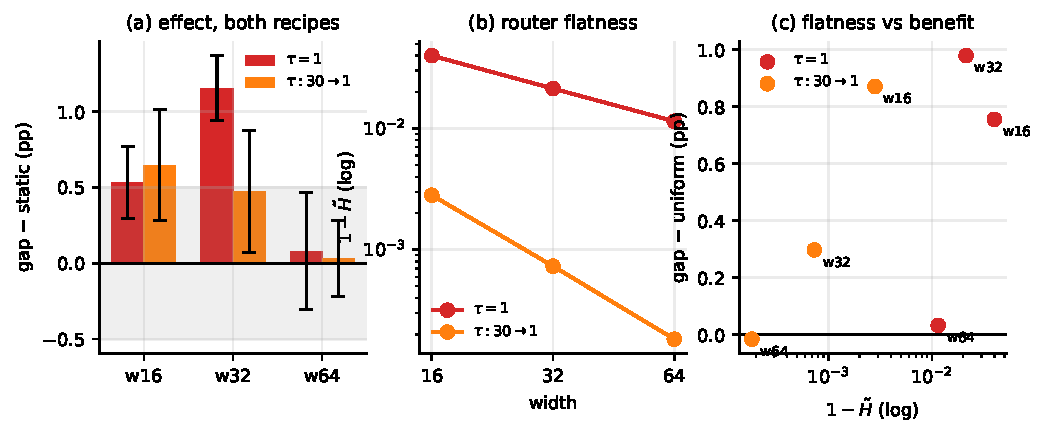
\includegraphics[width=\textwidth]{fig/f9_temp.pdf}
\caption{ResNet-18, CIFAR-100. (a) Routing effect under a constant and an annealed
temperature, \SI{95}{\percent} CIs. (b) Router flatness. (c) Flatness
against benefit over \texttt{uniform}; the two schedules do not lie on
one curve.}
\label{fig:temp}
\end{figure}

\begin{figure}[!htbp]\centering
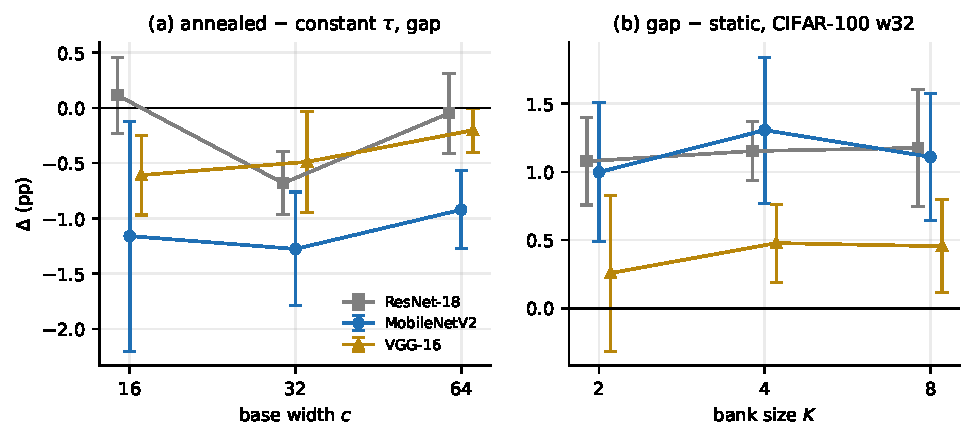
\includegraphics[width=\textwidth]{fig/g5_temp_k.pdf}
\caption{All three backbones, CIFAR-100. (a) Annealed minus constant
temperature for \texttt{gap}. (b) $\texttt{gap}-\texttt{static}$ at width 32
for $K\in\{2,4,8\}$. \SI{95}{\percent} CIs.}
\label{fig:mbtemp}
\end{figure}

With $\tau=1$ the softmax can move towards one-hot early in training,
starving most of the bank of gradient. DY-Conv anneals $\tau$ from 30 to 1
for this reason \citep{chen2020dynamic}. We repeated \texttt{gap} at all
three CIFAR-100 widths with that schedule on all three backbones
(Tables~\ref{tab:temp}, \ref{tab:mbtemp} and~\ref{tab:vgtemp},
Figures~\ref{fig:temp} and~\ref{fig:mbtemp}a).

\paragraph{Accuracy.} Annealing never raised accuracy detectably. On MobileNetV2 it
lowered \texttt{gap} at every width: \V{mbanA}\,pp at width 16
($p=\V{mbanAp}$), \V{mbanB}\,pp at width 32 ($p=\V{mbanBp}$) and
\V{mbanC}\,pp at width 64 ($p=\V{mbanCp}$), and the annealed runs ended at a
higher training loss at every width (\V{mblaA}, \V{mblaB}, \V{mblaC} against
\V{mblcA}, \V{mblcB}, \V{mblcC}). On ResNet-18 it lowered accuracy at width
32 (\V{anB}\,pp, $p=\V{anBp}$, again with a higher final training loss,
\V{laB} against \V{lcB}) and made no detectable difference at width 16
(\V{anA}\,pp, $p=\V{anAp}$) or width 64 (\V{anC}\,pp, $p=\V{anCp}$). On
VGG-16 it lowered \texttt{gap} at every width, by less than on
MobileNetV2: \V{vganA}\,pp at width 16 ($p=\V{vganAp}$), \V{vganB}\,pp at
width 32 ($p=\V{vganBp}$) and \V{vganC}\,pp at width 64 ($p=\V{vganCp}$),
with a slightly higher final training loss at every width (\V{vglaA},
\V{vglaB}, \V{vglaC} against \V{vglcA}, \V{vglcB}, \V{vglcC}). Over the nine
conditions annealing is significantly lower in \V{allannlower} and
significantly higher in \V{allannhigher}; the width-16 ResNet-18 point
estimate is positive but not distinguishable from zero. Backbone, dataset,
bank size and schedule length all differ from the DY-Conv setting, so this
is not evidence against their result.

\paragraph{Annealed routers against the constant mixture.} Compared with
\texttt{uniform}, the annealed router is equivalent to it on ResNet-18 at
width 64 (\V{anuC}\,pp, $p_{\text{TOST}}=\V{anuCT}$) and on MobileNetV2 at
width 32 (\V{mbanuB}\,pp); it is inconclusive on ResNet-18 at width 32
(\V{anuB}\,pp) and on MobileNetV2 at width 16 (\V{mbanuA}\,pp); and it
remains above \texttt{uniform} on ResNet-18 at width 16 (\V{anuA}\,pp,
$p=\V{anuAp}$) and on MobileNetV2 at width 64 (\V{mbanuC}\,pp). On VGG-16
it is inconclusive at width 16 (\V{vganuA}\,pp), equivalent at width 32
(\V{vganuB}\,pp) and above \texttt{uniform} at width 64 (\V{vganuC}\,pp,
$p=\V{vganuCp}$). On ResNet-18 and MobileNetV2 the annealed routers end
close to uniform by entropy (Section~\ref{sec:entropy}); the VGG-16
entropies are not available. One reading follows from
Proposition~\ref{prop:collapse}: a nearly constant mixture trains every
kernel toward a common update and so makes the bank homogeneous, which
leaves a router little to choose between. We did not test this, and
entropy was recorded only at the end of training, so we cannot say when
any router became flat.

\begin{table}[!htbp]\centering\small
\caption{ResNet-18: temperature ablation on CIFAR-100, \texttt{gap} arm. The last
two columns test whether the annealed router behaves like the constant
mixture.}
\label{tab:temp}
\begin{tabular}{r rr rl r rl rl}
\toprule
& \multicolumn{2}{c}{accuracy} & \multicolumn{2}{c}{annealed $-$ constant}
& \multicolumn{3}{c}{vs \texttt{static}} & \multicolumn{2}{c}{annealed vs \texttt{uniform}} \\
\cmidrule(lr){2-3}\cmidrule(lr){4-5}\cmidrule(lr){6-8}\cmidrule(lr){9-10}
width & $\tau=1$ & annealed & $\Delta$ & $p$ & $\tau=1$ & annealed & $p_{\text{TOST}}$ & $\Delta$ & verdict \\
\midrule
16 & 70.527 & 70.642 & +0.115 & 0.4313 & +0.532 & +0.647 & 0.8259 & +0.870 & higher \\
32 & 76.025 & 75.343 & -0.682 & 0.0017 & +1.153 & +0.472 & 0.4319 & +0.297 & inconclusive \\
64 & 78.418 & 78.370 & -0.048 & 0.7449 & +0.080 & +0.032 & 0.0025 & -0.017 & equivalent \\
\bottomrule
\end{tabular}
\end{table}

\begin{table}[!htbp]\centering\small
\caption{MobileNetV2: temperature ablation on CIFAR-100, \texttt{gap} arm.}
\label{tab:mbtemp}
\begin{tabular}{r rr rl r rl rl}
\toprule
& \multicolumn{2}{c}{accuracy} & \multicolumn{2}{c}{annealed $-$ constant}
& \multicolumn{3}{c}{vs \texttt{static}} & \multicolumn{2}{c}{annealed vs \texttt{uniform}} \\
\cmidrule(lr){2-3}\cmidrule(lr){4-5}\cmidrule(lr){6-8}\cmidrule(lr){9-10}
width & $\tau=1$ & annealed & $\Delta$ & $p$ & $\tau=1$ & annealed & $p$ & $\Delta$ & verdict \\
\midrule
16 & 68.272 & 67.112 & -1.160 & 0.0352 & +1.915 & +0.755 & 0.3286 & +0.162 & inconclusive \\
32 & 72.082 & 70.805 & -1.277 & 0.0014 & +1.307 & +0.030 & 0.8534 & +0.132 & equivalent \\
64 & 73.755 & 72.833 & -0.922 & 0.0011 & +1.360 & +0.438 & 0.0051 & +0.552 & higher \\
\bottomrule
\end{tabular}
\end{table}

\begin{table}[!htbp]\centering\small
\caption{VGG-16: temperature ablation on CIFAR-100, \texttt{gap} arm.}
\label{tab:vgtemp}
\begin{tabular}{r rr rl r rl rl}
\toprule
& \multicolumn{2}{c}{accuracy} & \multicolumn{2}{c}{annealed $-$ constant}
& \multicolumn{3}{c}{vs \texttt{static}} & \multicolumn{2}{c}{annealed vs \texttt{uniform}} \\
\cmidrule(lr){2-3}\cmidrule(lr){4-5}\cmidrule(lr){6-8}\cmidrule(lr){9-10}
width & $\tau=1$ & annealed & $\Delta$ & $p$ & $\tau=1$ & annealed & $p$ & $\Delta$ & verdict \\
\midrule
16 & 66.082 & 65.473 & -0.608 & 0.0075 & +0.863 & +0.255 & 0.0623 & +0.110 & inconclusive \\
32 & 71.797 & 71.308 & -0.488 & 0.0409 & +0.478 & -0.010 & 0.9274 & +0.138 & equivalent \\
64 & 74.992 & 74.790 & -0.202 & 0.0482 & +0.185 & -0.017 & 0.8955 & +0.172 & higher \\
\bottomrule
\end{tabular}
\end{table}

\section{Routing entropy}\label{sec:entropy}

\begin{figure}[!htbp]\centering
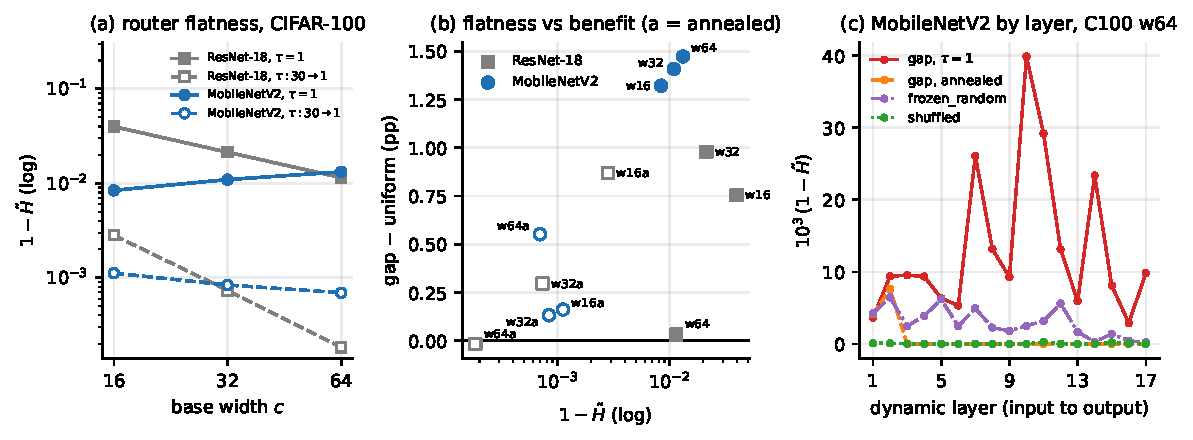
\includegraphics[width=\textwidth]{fig/g8_entropy.pdf}
\caption{Routing entropy on ResNet-18 and MobileNetV2. (a) Departure from uniform,
$1-\tilde H$, against width on CIFAR-100; open markers and dashed lines are
the annealed schedule. (b) $1-\tilde H$ against the benefit over
\texttt{uniform} in the six CIFAR-100 conditions of each backbone; ``a''
marks the annealed schedule. (c) MobileNetV2, CIFAR-100 width 64:
$1-\tilde H$ for each dynamic layer, mean over six seeds.}
\label{fig:mbent}
\end{figure}

Routing entropy (Section~\ref{sec:entdef}) is a natural statistic for
showing that a router is doing something. This section covers ResNet-18
and MobileNetV2 only: the VGG-16 entropies are stored in its result files,
which were not available for this draft.
Tables~\ref{tab:entben} and~\ref{tab:mbentben} set it against the benefit
each router delivers over \texttt{uniform}. Entropy compresses the signal
quadratically. Writing $z_k=1/K+\varepsilon_k$ with
$\sum_k\varepsilon_k=0$ and expanding to second order,
\begin{equation}
1-\tilde H\;\approx\;\frac{K}{2\log K}\sum_k\varepsilon_k^{2},
\label{eq:ent}
\end{equation}
so the deviations that carry input-dependent information enter squared.
At $1-\tilde H=\V{haA}$, for example, the root-mean-square deviation from
$1/K$ is about 0.022, so typical mixing weights lie in
[\V{spanlo}, \V{spanhi}], roughly \V{spanpct}\,\% of $1/K$, and entropy
reports that as 0.997. We call a layer \emph{flat} when
$\tilde H\ge0.9999$, which allows a root-mean-square deviation from $1/K$
of about 0.004, under \SI{2}{\percent} of $1/K$.

\paragraph{Within ResNet-18, entropy did not order the benefit reliably.}
Across its six CIFAR-100 conditions the rank correlation between
$1-\tilde H$ and the benefit over \texttt{uniform} is \V{rbrho} (Spearman,
$p=\V{rbrhop}$), which with six points is neither a demonstrated ordering
nor a demonstrated absence of one. The direct evidence is a counterexample.
At width 16 the two schedules give it
(Figure~\ref{fig:ent}): the constant router has $1-\tilde H=\V{hcA}$ and
beats \texttt{uniform} by \V{bcA}\,pp, while the annealed router is
\V{flA} times closer to uniform ($1-\tilde H=\V{haA}$) and beats it by
\V{anuA}\,pp ($p=\V{anuAp}$).

\paragraph{Within MobileNetV2, it did.} The same correlation is
\V{mbrho} ($p=\V{mbrhop}$), and the width-16 counterexample does not recur:
the annealed router is \V{mbflA} times closer to uniform and delivers less
(\V{mbbaA}\,pp, $p=\V{mbbapA}$, against \V{mbbcA}\,pp). Inside the annealed
schedule the order is reversed: the router closest to uniform, at width
64, is the only annealed one whose benefit is significant (\V{mbbaC}\,pp,
$p=\V{mbbapC}$, against \V{mbbaA} and \V{mbbaB}\,pp at widths 16 and 32);
the differences between these three benefits were not tested.

\paragraph{Across backbones, the same entropy, a different benefit.} On
CIFAR-100 at width 64 the constant-temperature routers of the two
backbones are almost equally far from uniform ($1-\tilde H=\V{rbhcC}$ on
ResNet-18, \V{mbhcC} on MobileNetV2). The ResNet-18 router is equivalent to
\texttt{uniform} (\V{rbguC}\,pp); the MobileNetV2 router beats it by
\V{mbguC}\,pp ($p$\,\V{mbguCp}). The width trends are opposite: from width
16 to 64 the ResNet-18 router moves towards uniform (\V{rbhcA} to
\V{rbhcC}) and the MobileNetV2 router away from it (\V{mbhcA} to
\V{mbhcC}; Figure~\ref{fig:mbent}a).

\paragraph{After annealing, routers end close to uniform.} Under the
annealed schedule the MobileNetV2 router is flat in \V{mbflatAmin} to
\V{mbflatAmax} of its \V{mbnlayers} dynamic layers, in every seed at every
width; across all eighteen annealed runs the only layers that are ever not
flat are layers \V{mbannlayers}, counted from the input
(Figure~\ref{fig:mbent}c, Table~\ref{tab:mblayer}). Under a constant
temperature \V{mbflatCmin} to \V{mbflatCmax} layers are flat. The
temperature reaches 1 at epoch 10, so these routers end close to uniform
after 140 epochs at the same temperature as the constant ones. On
ResNet-18 the annealed router at width 64 ends at $1-\tilde H=\V{haC}$ and
is equivalent to \texttt{uniform}; on MobileNetV2 the annealed router at
width 64 ends at $1-\tilde H=\V{mbhaC}$ and still beats \texttt{uniform} by
\V{mbbaC}\,pp. A very low departure from uniform thus accompanied no
benefit in one case and a significant benefit in the other.

\paragraph{Conclusion.} Entropy can move with the benefit, as within
MobileNetV2, but it did not reliably within ResNet-18, and almost the same
value accompanies very different benefits on the two backbones. A value of
$\tilde H$ below one is not evidence that routing is useful, and a value
near one is not evidence that it is not. These statements rest on 16
images per run, measured once at the end of training
(Section~\ref{sec:entdef}).

\begin{figure}[!htbp]\centering
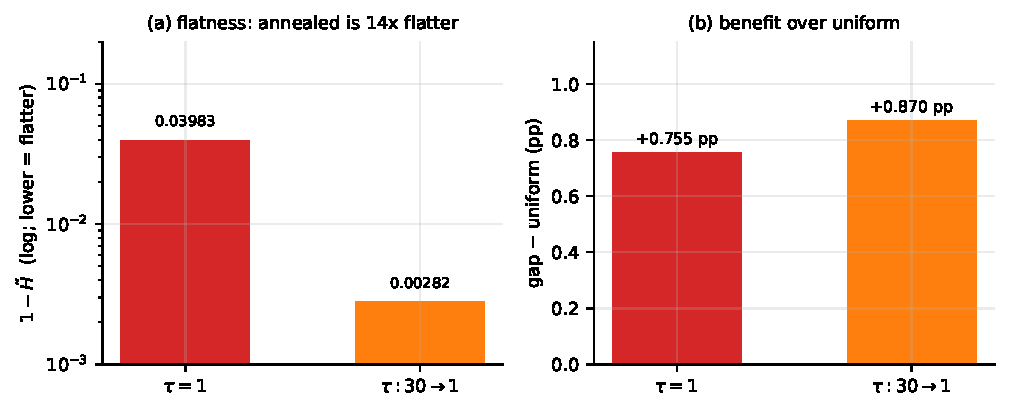
\includegraphics[width=0.74\textwidth]{fig/f10_entropy.pdf}
\caption{ResNet-18, CIFAR-100, width 16. The annealed router is \V{flA}
times closer to uniform by entropy and delivers the larger benefit over
\texttt{uniform}. On MobileNetV2 the order reverses
(Table~\ref{tab:mbentben}).}
\label{fig:ent}
\end{figure}

\begin{table}[!htbp]\centering\small
\caption{ResNet-18: routing entropy against the benefit it is taken to
indicate, CIFAR-100. RMS dev is the root-mean-square deviation of the mixing
weights from $1/K$, recovered from Eq.~\eqref{eq:ent}.}
\label{tab:entben}
\begin{tabular}{r l rrr rl}
\toprule
width & $\tau$ & $\tilde H$ & $1-\tilde H$ & RMS dev & \texttt{gap}$-$\texttt{uniform} (pp) & $p$ \\
\midrule
16 & $1$ & 0.96017 & 0.03983 & 0.0831 & +0.755 & 0.0023 \\
16 & $30\!\to\!1$ & 0.99718 & 0.00282 & 0.0221 & +0.870 & 0.0044 \\
32 & $1$ & 0.97868 & 0.02132 & 0.0608 & +0.978 & 0.0010 \\
32 & $30\!\to\!1$ & 0.99927 & 0.00073 & 0.0113 & +0.297 & 0.0810 \\
64 & $1$ & 0.98853 & 0.01147 & 0.0446 & +0.032 & 0.7752 \\
64 & $30\!\to\!1$ & 0.99982 & 0.00018 & 0.0056 & -0.017 & 0.8369 \\
\bottomrule
\end{tabular}
\end{table}

\begin{table}[!htbp]\centering\small
\caption{MobileNetV2: routing entropy against the benefit over
\texttt{uniform}, for every \texttt{gap} group that has a \texttt{uniform}
arm. RMS dev is recovered from Eq.~\eqref{eq:ent} as in
Table~\ref{tab:entben}. Flat layers: dynamic layers (of \V{mbnlayers})
with $\tilde H\ge0.9999$, range over seeds.}
\label{tab:mbentben}
\resizebox{\textwidth}{!}{%
\begin{tabular}{l r l rrr r rll}
\toprule
dataset & width & $\tau$ & $\tilde H$ & $1-\tilde H$ & RMS dev & flat layers & \texttt{gap}$-$\texttt{uniform} (pp) & $p$ & verdict \\
\midrule
CIFAR-100 & 16 & $1$ & 0.99159 & 0.00841 & 0.0382 & 6--7 & +1.322 & 0.0011 & higher \\
CIFAR-100 & 16 & $30\!\to\!1$ & 0.99888 & 0.00112 & 0.0139 & 15--16 & +0.162 & 0.7242 & inconclusive \\
CIFAR-100 & 32 & $1$ & 0.98906 & 0.01094 & 0.0435 & 4--7 & +1.408 & 0.0002 & higher \\
CIFAR-100 & 32 & $30\!\to\!1$ & 0.99916 & 0.00084 & 0.0120 & 15 & +0.132 & 0.4319 & equivalent \\
CIFAR-100 & 64 & $1$ & 0.98680 & 0.01320 & 0.0478 & 2--4 & +1.473 & $<10^{-4}$ & higher \\
CIFAR-100 & 64 & $30\!\to\!1$ & 0.99931 & 0.00069 & 0.0110 & 15--16 & +0.552 & 0.0133 & higher \\
Tiny-ImageNet & 32 & $1$ & 0.99267 & 0.00733 & 0.0356 & 3--5 & +1.888 & 0.0008 & higher \\
Tiny-ImageNet & 64 & $1$ & 0.99160 & 0.00840 & 0.0382 & 2--5 & +1.807 & 0.0014 & higher \\
\bottomrule
\end{tabular}}
\end{table}

\section{The pre-registered predictions}\label{sec:prereg}

Of the \V{allpred} predictions recorded, dated, before the runs that test
them, \V{allpredfail} failed. The ResNet-18 prediction that the effect
would vanish on Tiny-ImageNet at width 64 failed (Table~\ref{tab:predict},
Section~\ref{sec:null}). Tables~\ref{tab:mbprereg} and~\ref{tab:vgprereg}
give the three predictions made for each of MobileNetV2 and VGG-16,
recorded on 30 September 2026 before any run of either.

\paragraph{P1, the bank term is equivalent to zero in all five
conditions.} It failed on both: the bank term was equivalent to zero in
\V{mbP1} of five conditions on MobileNetV2 and \V{vgP1} of five on VGG-16.
The inconclusive conditions are not evidence of a bank effect, since none
is significant, and finding~1 claims only that no bank effect was
detected; but the prediction was equivalence, and we score it as stated.

\paragraph{P2, the plain network of twice the width beats the routed one
in all three pairs.} It failed on MobileNetV2, holding in \V{mbP2} of three
pairs, and held on VGG-16, in \V{vgP2} of three, as the same comparison
did on ResNet-18 (Section~\ref{sec:cost}).

\paragraph{P3, the routing term is significant in at least three of five
conditions.} It held on both: in \V{mbP3} of five conditions on
MobileNetV2 and \V{vgP3} of five on VGG-16.

The two gates, which required the first static run of each backbone to
reach \SI{65}{\percent} on CIFAR-100, were passed (\V{mbgate} and
\V{vggate}\,\%).

\begin{table}[!htbp]\centering\small
\caption{MobileNetV2: predictions recorded on 30 September 2026, before
any MobileNetV2 run, and the outcomes.}
\label{tab:mbprereg}
\begin{tabular}{l p{8.2cm} l l}
\toprule
& prediction & measured & outcome \\
\midrule
P1 & The bank term (\texttt{uniform}$-$\texttt{static}) is equivalent to zero (TOST, $\pm$\SI{0.5}{pp}) in each of the five conditions & 2 of 5 & failed \\
P2 & \texttt{static} at width $2c$ is more accurate than \texttt{gap} at width $c$ in each of the three pairs & 1 of 3 & failed \\
P3 & The routing term is positive with $p<0.05$ in at least three of the five conditions & 5 of 5 & held \\
\bottomrule
\end{tabular}
\end{table}

\begin{table}[!htbp]\centering\small
\caption{VGG-16: predictions recorded on 30 September 2026, before any
VGG-16 run, and the outcomes.}
\label{tab:vgprereg}
\begin{tabular}{l p{8.2cm} l l}
\toprule
& prediction & measured & outcome \\
\midrule
P1 & The bank term (\texttt{uniform}$-$\texttt{static}) is equivalent to zero (TOST, $\pm$\SI{0.5}{pp}) in each of the five conditions & 2 of 5 & failed \\
P2 & \texttt{static} at width $2c$ is more accurate than \texttt{gap} at width $c$ in each of the three pairs & 3 of 3 & held \\
P3 & The routing term is positive with $p<0.05$ in at least three of the five conditions & 4 of 5 & held \\
\bottomrule
\end{tabular}
\end{table}

\section{Result by result}\label{sec:summary}

Table~\ref{tab:contra} lists the main results on the three backbones. Of
its \V{ncontra} rows, \V{ncontraHold} hold on all three backbones,
\V{ncontraBD} depend on the backbone (two of them measured on ResNet-18 and
MobileNetV2 only, because the VGG-16 entropies are not available), and
the last compares backbones directly.

\begin{table}[!htbp]\centering\small
\caption{The main results on the three backbones. Differences are in pp
and paired by seed. Status: \emph{holds on all three},
\emph{backbone-dependent} or \emph{across backbones} (a comparison
between them).}
\label{tab:contra}
\resizebox{\textwidth}{!}{%
\begin{tabular}{l l l l l}
\toprule
result & ResNet-18 & MobileNetV2 & VGG-16 & status \\
\midrule
Bank term ($\texttt{uniform}-\texttt{static}$) & equivalent in 5 of 5 & equivalent in 2 of 5; never significant (largest +0.59) & equivalent in 2 of 5; never significant (largest +0.25) & holds on all three (weaker on MobileNetV2 and VGG-16) \\
Routing term significant & 4 of 5 & 5 of 5 & 4 of 5 & holds on all three \\
$\texttt{gap}-\texttt{static}$, CIFAR-100 w64 & +0.08 (equivalent) & +1.36 (higher) & +0.18 (equivalent) & \textbf{backbone-dependent} \\
Plain $2c$ beats \texttt{gap} $c$ (3 pairs) & 3 of 3 (+4.35, +2.31, +2.52) & 1 of 3 (+2.50, +0.31, +0.15) & 3 of 3 (+5.24, +3.01, +2.49) & \textbf{backbone-dependent} \\
Annealed $-$ constant $\tau$ (w16, 32, 64) & +0.11, -0.68, -0.05 & -1.16, -1.28, -0.92 & -0.61, -0.49, -0.20 & holds on all three (never significantly higher) \\
\texttt{gap} / \texttt{frozen\_random} $-$ \texttt{uniform}, w64 & +0.03 / +0.13 (equivalent / equivalent) & +1.47 / +1.63 (higher / higher) & +0.37 / +0.09 (higher / equivalent) & \textbf{backbone-dependent} \\
$K=8$ vs $K=2$, CIFAR-100 w32 & +0.10 (equivalent) & +0.11 (inconclusive) & +0.20 (inconclusive) & holds on all three \\
Entropy counterexample, CIFAR-100 w16 & annealed 14$\times$ flatter, larger benefit (+0.87 vs +0.76) & annealed 7.5$\times$ flatter, smaller benefit (+0.16 vs +1.32) & not available (no result files) & \textbf{backbone-dependent} (two backbones) \\
Constant-$\tau$ $1-\tilde H$ as width grows (w16, 32, 64) & 0.0398, 0.0213, 0.0115 (flattens) & 0.0084, 0.0109, 0.0132 (sharpens) & not available (no result files) & \textbf{backbone-dependent} (two backbones) \\
Same $1-\tilde H$, CIFAR-100 w64, \texttt{gap}$-$\texttt{uniform} & 0.0115: +0.03 (equivalent) & 0.0132: +1.47 (higher) & not available (no result files) & across backbones \\
\bottomrule
\end{tabular}}
\end{table}

\paragraph{An interpretation.} On MobileNetV2 the router does not need to
be trained, and annealing, which keeps the mixture nearly constant early in
training and leaves it close to uniform at the end, removes most of the
benefit. Both fit the reading that what matters is that the mixture differ
across images from early in training, not that it be optimised. The other
backbones do not support this reading everywhere: on ResNet-18 at width 16
the annealed router kept the full benefit over \texttt{uniform}
(\V{anuA} against \V{bcA}\,pp), and on VGG-16 only the trained router
departs from the constant mixture. None of these experiments was designed
to test the reading, and we state it as an interpretation only.

\paragraph{Why the backbones may differ.} ResNet-18 and VGG-16 agree with
each other and differ from MobileNetV2 on two of the three
backbone-dependent accuracy results: the null at CIFAR-100 width 64, and
the plain network of twice the width winning every pair. On the third, the
routing controls, each backbone gives a different pattern. Several
properties separate ResNet-18 and VGG-16 from MobileNetV2 at once: the share of parameters in dynamic layers (nearly all
against \V{mbdynshare}\,\%), full against depthwise convolution in those
layers, the size of the router relative to the bank (\V{vgrouterpct}\,\% of
the static network on VGG-16 against \V{mbrouterpct}\,\% on MobileNetV2),
and how close the network comes to fitting its training set under this
recipe. Residual connections are not among them, since VGG-16 has none and
ResNet-18 has them. None of the other properties was isolated here, so
none of the backbone-dependent results can be attributed to one of them.
The two remaining backbones vary them further: ResNet-50 keeps about half
its parameters in full dynamic convolutions, and ConvNeXt-Tiny makes only
its depthwise $7\times7$ layers dynamic.

\section{Threats to validity}\label{sec:threats}

\paragraph{Scale.} Both datasets are low-resolution and every run fits on
one consumer GPU. Behaviour at ImageNet scale is untested and cannot be
tested on this hardware.

\paragraph{Three backbones.} The backbones disagree on \V{ncontraBD} of the
\V{ncontra} results in Table~\ref{tab:contra}, so what holds on all three
is the minimum that can be claimed. The same program on ResNet-50 and
ConvNeXt-Tiny was pre-registered on 30 September 2026 and is running; its
results will be added as they complete, whatever they show.

\paragraph{Placement and router size on MobileNetV2.} Copying the
ResNet-18 rule makes only the depthwise layers of MobileNetV2 dynamic,
\V{mbdynshare}\,\% of its parameters, and its router is larger than the
bank. A different rule, such as making every convolution but the stem
dynamic, could change the MobileNetV2 results. The frozen-router control
shows that the trainable router parameters do not produce the gain there.

\paragraph{Entropy sample.} The routing statistics are overwritten at each
test batch, so every recorded entropy, on ResNet-18 and MobileNetV2,
describes the last batch of the unshuffled test set: the same 16 images in
every run on a dataset. Comparisons between arms, widths and schedules are
therefore made on identical inputs, and the spread across seeds is small
(Tables~\ref{tab:entw64} and~\ref{tab:mbentw64}), but no entropy here is a
test-set average. The trained weights were not kept, so the entropies
cannot be recomputed on the full test set. No accuracy is affected. The
VGG-16 entropies, recorded the same way, are in result files that were not
available for this draft.

\paragraph{One recipe.} All three backbones use the same recipe. The
MobileNetV2 static arms never approach zero training loss under it, and a
recipe tuned for MobileNetV2 could change where routing helps.

\paragraph{Initialisation.} On ResNet-18, static convolutions in the
\texttt{static} arm, and the static stem, shortcut and head layers in
every arm, keep PyTorch's default initialisation (Kaiming-uniform with
$a=\sqrt5$), while every kernel of every dynamic bank is initialised
Kaiming-normal with fan-out. The ResNet-18 bank term therefore compares
two initialisations as well as a bank against a single kernel. The routing
term is not affected: both arms have identically initialised banks.
MobileNetV2 and VGG-16, and the two remaining backbones, initialise static
and bank kernels with one scheme, and the MobileNetV2 and VGG-16 bank
terms, which are free of the mismatch, also show no bank effect.

\paragraph{Not a reproduction of a published system.} The layer is a
dynamic convolution of the CondConv and DY-Conv form. No published
implementation of ODConv, FDConv or KernelWarehouse was run, and the
conclusions concern dynamic convolution of this form.

\paragraph{Global routing.} Every router here uses a global descriptor.
Spatially resolved routing is not covered.

\paragraph{One random router.} The \texttt{frozen\_random} control uses a
single random draw, identical across seeds, in one condition. It shows that
a random router can match a trained one on MobileNetV2, not how often; on
VGG-16 the same kind of draw did not depart from the constant mixture.

\paragraph{Scope of the ablations.} The bank-size, temperature and
routing-control groups were run on CIFAR-100 only, and each of their
results is stated as a CIFAR-100 result. On ResNet-18 these groups were
added in stages; for MobileNetV2 and VGG-16 the same program, including
this scope, was fixed in the pre-registration before any run. A
Tiny-ImageNet run of the routed network costs 4 to 10 times a CIFAR-100
run at the same width (Tables~\ref{tab:config}, \ref{tab:mbconfig}
and~\ref{tab:vgconfig}); for ResNet-18 and MobileNetV2 alone, repeating
these groups on Tiny-ImageNet would take roughly one and a half times the
GPU time those two backbones used. Tiny-ImageNet has a different role in
the design: it tests whether the split into bank and routing terms holds
on a harder dataset, and it tests the recorded saturation prediction.

\paragraph{One annealing schedule.} Section~\ref{sec:temp} compares a
constant temperature with one linear schedule.

\paragraph{Stored and effective parameters.} By
Proposition~\ref{prop:collapse} the \texttt{uniform} arm has the effective
capacity of a plain network. The twice-the-width comparisons of
Section~\ref{sec:matched} use stored parameters; the equal-compute
comparison of Section~\ref{sec:cost} favours routing on all three
backbones.

\paragraph{The CIFAR-100 width-64 null is unexplained.} On ResNet-18 it is
well powered, on both ResNet-18 and VGG-16 it is a positive equivalence
and does not depend on the temperature schedule, its stated explanation
failed a recorded test, and it does not appear on MobileNetV2
(Section~\ref{sec:null}).

\paragraph{Provenance and corrections.} ResNet-18 final accuracies were
transcribed from the training logs, which print them verbatim, and every
figure and table is generated from those per-seed values; MobileNetV2
values are parsed from its log and checked against its result files, and
VGG-16 values are parsed from its log and checked against its runner log
(Section~\ref{sec:method}). During the ResNet-18 analysis, three scripts
grouped results by width alone, which merged runs from the two datasets and
from different bank sizes; this was detected when a comparison paired one
dataset's \texttt{uniform} arm with the other's \texttt{static} arm, and
every number in this report was recomputed from per-seed values keyed on
dataset, width, bank size and schedule. Summary sentences printed by the
analysis scripts were also found to over-read non-significant orderings on
four occasions; this report relies on the per-comparison statistics only.
The report generator was later rewritten to read the result files
directly; on the 24 ResNet-18 width-64 result files checked it reproduces
the transcribed accuracies and routing entropies exactly. Every
transcribed ResNet-18 accuracy was re-checked on 19 October 2026 against
the per-run lines of the logs or against the result files, except those
for Tiny-ImageNet at width 32 \texttt{static} and \texttt{gap}, which were
checked against the printed means and standard deviations. The ResNet-18
routing entropies for CIFAR-100 widths 16 and 32 and for the three annealed
groups were transcribed from result files that are not in the
accompanying archive, so they cannot be re-derived from it; only the
width-64 files are. An earlier version of this report printed stored
parameter counts with a third decimal that had not been measured, and six
of nineteen were off by up to \SI{0.005}{M} (for example \SI{0.708}{M} for
\SI{0.713}{M}); the counts here are counted from the model definition and
agree with the training logs to the two decimals they print. No comparison
changes.

\section{Conclusion}

Across three backbones, two datasets and \V{totruns} runs, the gain of
dynamic convolution does not come from its kernel bank. A uniformly mixed
bank was never significantly better or worse than a plain network, and was
equivalent to one in \V{allbankeq} of fifteen backbone and condition pairs.
Dynamic convolution beat the plain network in \V{alleff} of the fifteen,
and in \V{alleffrout} of those the routing term was significant on its
own; on CIFAR-100 at width 32, banks larger than $K=2$ added nothing that
we could detect on any backbone. Whether the router had to be trained
depended on the backbone: on MobileNetV2 a router frozen at random
initialisation did as well as a trained one, provided each image was
routed by its own descriptor, while on VGG-16 only the trained router
departed from the constant mixture.

How much this is worth depends on the backbone and on the cost held
fixed. A plain network of twice the width, which on ResNet-18 and VGG-16
has the same number of parameters as the routed one, did better in all six
pairs there, by \V{eqpmin} to \V{eqpmax}\,pp, while on MobileNetV2, where
twice the width means \V{mbpinvlo} to \V{mbpinvhi} times the parameters, it
won only one of three. At equal width, for at most \V{rbmacextra},
\V{mbmacextra} and \V{vgmacextra}\,\% more compute, routing beat the plain
network in \V{rbeqmac}, \V{mbeqmac} and \V{vgeqmac} of five conditions. The
two pairs without an effect, CIFAR-100 at width 64 on ResNet-18 and on
VGG-16, remain unexplained.

Two common practices did not help. On CIFAR-100, annealing the softmax
temperature never detectably raised accuracy and lowered it in
\V{allannlower} of nine conditions. Routing entropy, measured on ResNet-18
and MobileNetV2, did not reliably indicate whether routing helped: it
ordered the benefit within MobileNetV2 but not reliably within ResNet-18,
and almost the same entropy accompanied benefits of \V{rbguC} and
\V{mbguC}\,pp on the two backbones. Of our \V{allpred} recorded
predictions, \V{allpredfail} failed.

\paragraph{Reproducibility.} \V{totruns} runs (\V{nruns} ResNet-18,
\V{mbruns} MobileNetV2, \V{vgruns} VGG-16), \V{totgpuh} GPU-hours, one
RTX 4070 Ti. Code, the pre-registrations, the dated prediction, the gate
ledgers with recorded evidence, the 132 MobileNetV2 result files, the 24
ResNet-18 result files of CIFAR-100 width 64, the VGG-16 training and
runner logs and every per-seed value accompany this report. The other 108
ResNet-18 runs are represented by the per-seed values transcribed from
their logs, and the 132 VGG-16 runs by their logs, whose result files were
not available for this draft (Section~\ref{sec:threats}).

\FloatBarrier
\begin{thebibliography}{99}\small
\bibitem[Arora et~al.(2018)]{arora2018optimization} S.~Arora, N.~Cohen, and E.~Hazan. On the optimization of deep networks: Implicit acceleration by overparameterization. In \emph{ICML}, 2018.
\bibitem[Chen et~al.(2021)]{chen2021drconv} J.~Chen, X.~Wang, Z.~Guo, X.~Zhang, and J.~Sun. Dynamic region-aware convolution. In \emph{CVPR}, 2021.
\bibitem[Chen et~al.(2025)]{chen2025fdconv} L.~Chen, L.~Gu, L.~Li, C.~Yan, and Y.~Fu. Frequency dynamic convolution for dense image prediction. In \emph{CVPR}, pages 30178--30188, 2025.
\bibitem[Chen et~al.(2020)]{chen2020dynamic} Y.~Chen, X.~Dai, M.~Liu, D.~Chen, L.~Yuan, and Z.~Liu. Dynamic convolution: Attention over convolution kernels. In \emph{CVPR}, pages 11030--11039, 2020.
\bibitem[Ding et~al.(2019)]{ding2019acnet} X.~Ding, Y.~Guo, G.~Ding, and J.~Han. ACNet: Strengthening the kernel skeletons for powerful CNN via asymmetric convolution blocks. In \emph{ICCV}, 2019.
\bibitem[Ding et~al.(2021)]{ding2021repvgg} X.~Ding, X.~Zhang, N.~Ma, J.~Han, G.~Ding, and J.~Sun. RepVGG: Making VGG-style ConvNets great again. In \emph{CVPR}, 2021.
\bibitem[He et~al.(2023)]{he2023sdconv} S.~He, C.~Jiang, D.~Dong, and L.~Ding. SD-Conv: Towards the parameter-efficiency of dynamic convolution. In \emph{WACV}, 2023.
\bibitem[He et~al.(2016)]{he2016deep} K.~He, X.~Zhang, S.~Ren, and J.~Sun. Deep residual learning for image recognition. In \emph{CVPR}, 2016.
\bibitem[Krizhevsky(2009)]{krizhevsky2009} A.~Krizhevsky. Learning multiple layers of features from tiny images. Technical report, University of Toronto, 2009.
\bibitem[Lakens(2017)]{lakens2017} D.~Lakens. Equivalence tests: A practical primer for $t$ tests, correlations, and meta-analyses. \emph{Social Psychological and Personality Science}, 8(4):355--362, 2017.
\bibitem[Le and Yang(2015)]{le2015tiny} Y.~Le and X.~Yang. Tiny ImageNet visual recognition challenge. CS231N course report, Stanford University, 2015.
\bibitem[Li and Yao(2024)]{li2024kernelwarehouse} C.~Li and A.~Yao. KernelWarehouse: Rethinking the design of dynamic convolution. In \emph{ICML}, PMLR 235:29201--29221, 2024.
\bibitem[Li et~al.(2022)]{li2022odconv} C.~Li, A.~Zhou, and A.~Yao. Omni-dimensional dynamic convolution. In \emph{ICLR}, 2022.
\bibitem[Li et~al.(2021)]{li2021dcd} Y.~Li, Y.~Chen, X.~Dai, M.~Liu, D.~Chen, Y.~Yu, L.~Yuan, Z.~Liu, M.~Chen, and N.~Vasconcelos. Revisiting dynamic convolution via matrix decomposition. In \emph{ICLR}, 2021.
\bibitem[Sandler et~al.(2018)]{sandler2018mobilenetv2} M.~Sandler, A.~Howard, M.~Zhu, A.~Zhmoginov, and L.-C. Chen. MobileNetV2: Inverted residuals and linear bottlenecks. In \emph{CVPR}, 2018.
\bibitem[Schuirmann(1987)]{schuirmann1987} D.~J. Schuirmann. A comparison of the two one-sided tests procedure and the power approach for assessing the equivalence of average bioavailability. \emph{Journal of Pharmacokinetics and Biopharmaceutics}, 15(6):657--680, 1987.
\bibitem[Simonyan and Zisserman(2015)]{simonyan2015vgg} K.~Simonyan and A.~Zisserman. Very deep convolutional networks for large-scale image recognition. In \emph{ICLR}, 2015.
\bibitem[Wilcoxon(1945)]{wilcoxon1945} F.~Wilcoxon. Individual comparisons by ranking methods. \emph{Biometrics Bulletin}, 1(6):80--83, 1945.
\bibitem[Yang et~al.(2019)]{yang2019condconv} B.~Yang, G.~Bender, Q.~V. Le, and J.~Ngiam. CondConv: Conditionally parameterized convolutions for efficient inference. In \emph{NeurIPS}, 2019.
\bibitem[Zhang et~al.(2017)]{zhang2017} C.~Zhang, S.~Bengio, M.~Hardt, B.~Recht, and O.~Vinyals. Understanding deep learning requires rethinking generalization. In \emph{ICLR}, 2017.
\end{thebibliography}

\clearpage
\appendix
\section{Complete results: ResNet-18}

\begin{figure}[!htbp]\centering
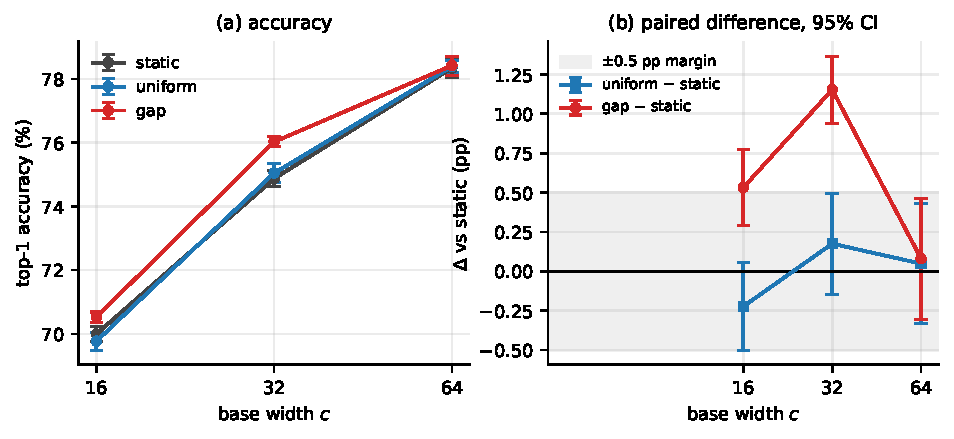
\includegraphics[width=\textwidth]{fig/f1_sweep.pdf}
\caption{ResNet-18, CIFAR-100. (a) Accuracy against base width, $\pm1$ standard
deviation over six seeds. (b) Paired difference from \texttt{static} with
\SI{95}{\percent} confidence intervals.}
\label{fig:sweep}
\end{figure}

\begin{figure}[!htbp]\centering
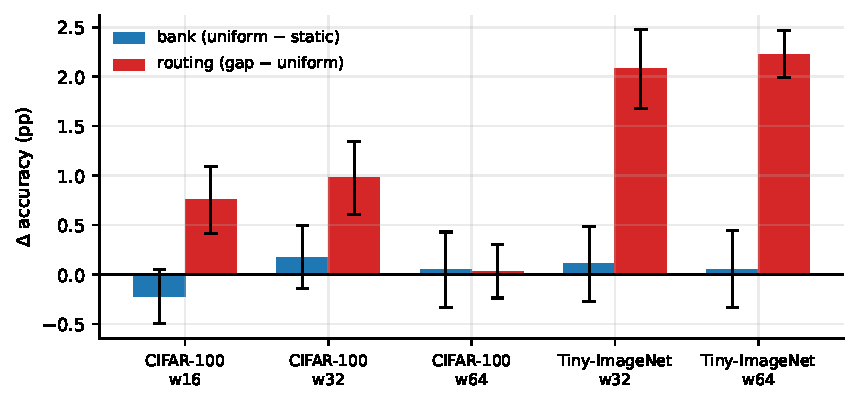
\includegraphics[width=0.84\textwidth]{fig/f4_decomp.pdf}
\caption{ResNet-18: decomposition of the effect of dynamic convolution into the
bank ($\texttt{uniform}-\texttt{static}$) and routing
($\texttt{gap}-\texttt{uniform}$), five conditions, \SI{95}{\percent}
CIs.}
\label{fig:decomp}
\end{figure}

\begin{figure}[h]\centering
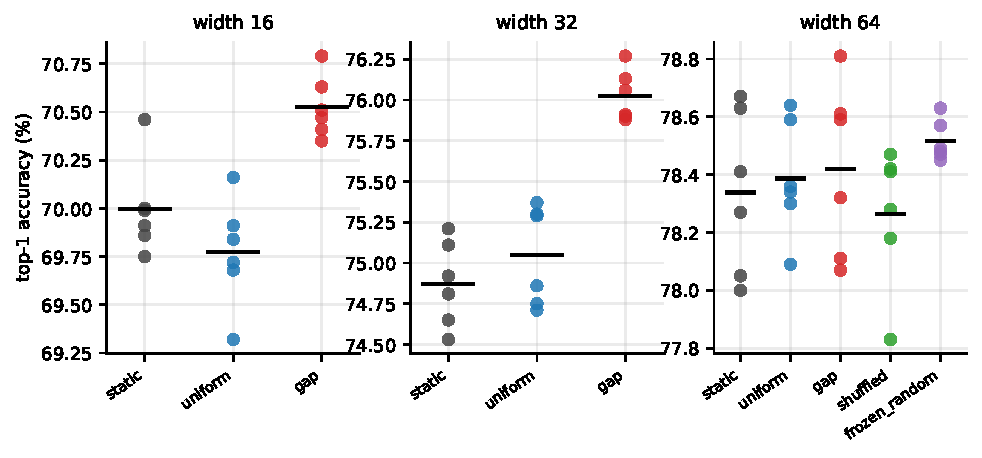
\includegraphics[width=\textwidth]{fig/f2_allruns.pdf}
\caption{ResNet-18: every CIFAR-100 run at $K=4$ and $\tau=1$; bars are arm means.}
\label{fig:allruns}
\end{figure}

\begin{table}[h]\centering\scriptsize
\caption{ResNet-18: every run at $K=4$ and $\tau=1$: final-epoch top-1 accuracy
(\si{\percent}) for each seed, with mean and sample standard deviation.}
\label{tab:allruns}
\begin{tabular}{l r l rrrrrr rr}
\toprule
dataset & width & arm & s0 & s1 & s2 & s3 & s4 & s5 & mean & sd \\
\midrule
CIFAR-100 & 16 & \texttt{static} & 69.91 & 69.75 & 69.86 & 70.46 & 70.00 & 69.99 & 69.995 & 0.246 \\
CIFAR-100 & 16 & \texttt{uniform} & 69.68 & 69.32 & 69.84 & 69.91 & 69.72 & 70.16 & 69.772 & 0.279 \\
CIFAR-100 & 16 & \texttt{gap} & 70.35 & 70.51 & 70.41 & 70.63 & 70.79 & 70.47 & 70.527 & 0.160 \\
CIFAR-100 & 32 & \texttt{static} & 74.81 & 74.65 & 74.53 & 74.92 & 75.11 & 75.21 & 74.872 & 0.262 \\
CIFAR-100 & 32 & \texttt{uniform} & 75.29 & 74.86 & 74.75 & 75.30 & 74.71 & 75.37 & 75.047 & 0.305 \\
CIFAR-100 & 32 & \texttt{gap} & 76.13 & 75.88 & 75.91 & 75.90 & 76.27 & 76.06 & 76.025 & 0.156 \\
CIFAR-100 & 64 & \texttt{static} & 78.05 & 78.67 & 78.63 & 78.27 & 78.00 & 78.41 & 78.338 & 0.284 \\
CIFAR-100 & 64 & \texttt{uniform} & 78.64 & 78.59 & 78.34 & 78.30 & 78.36 & 78.09 & 78.387 & 0.202 \\
CIFAR-100 & 64 & \texttt{gap} & 78.59 & 78.81 & 78.11 & 78.61 & 78.07 & 78.32 & 78.418 & 0.299 \\
CIFAR-100 & 64 & \texttt{shuffled} & 78.42 & 77.83 & 78.18 & 78.41 & 78.47 & 78.28 & 78.265 & 0.238 \\
CIFAR-100 & 64 & \texttt{frozen\_random} & 78.47 & 78.49 & 78.48 & 78.63 & 78.45 & 78.57 & 78.515 & 0.070 \\
Tiny-ImageNet & 32 & \texttt{static} & 61.93 & 61.61 & 61.57 & 61.46 & 61.27 & 61.52 & 61.560 & 0.217 \\
Tiny-ImageNet & 32 & \texttt{uniform} & 61.52 & 61.53 & 61.55 & 61.62 & 61.66 & 62.12 & 61.667 & 0.229 \\
Tiny-ImageNet & 32 & \texttt{gap} & 63.53 & 64.20 & 63.61 & 63.58 & 63.91 & 63.64 & 63.745 & 0.260 \\
Tiny-ImageNet & 64 & \texttt{static} & 66.29 & 66.59 & 65.88 & 65.97 & 66.63 & 66.23 & 66.265 & 0.309 \\
Tiny-ImageNet & 64 & \texttt{uniform} & 66.27 & 66.27 & 66.41 & 66.21 & 66.22 & 66.53 & 66.318 & 0.126 \\
Tiny-ImageNet & 64 & \texttt{gap} & 68.73 & 68.35 & 68.42 & 68.55 & 68.71 & 68.52 & 68.547 & 0.152 \\
\bottomrule
\end{tabular}
\end{table}

\begin{table}[h]\centering\small
\caption{ResNet-18: paired comparisons against \texttt{static}, $n=6$. $p_W$ is the
Wilcoxon signed-rank test, which cannot fall below 0.031 at this $n$.}
\label{tab:vsstatic}
\resizebox{\textwidth}{!}{%
\begin{tabular}{l r l r l ll r l l}
\toprule
dataset & width & arm & $\Delta$ (pp) & \SI{95}{\percent} CI & $p_t$ & $p_W$ & $d_z$ & $p_{\text{TOST}}$ & verdict \\
\midrule
CIFAR-100 & 16 & \texttt{uniform} & -0.223 & [-0.500, +0.054] & 0.0931 & 0.0938 & -0.85 & 0.0251 & equivalent \\
CIFAR-100 & 16 & \texttt{gap} & +0.532 & [+0.292, +0.771] & 0.0023 & 0.0312 & +2.33 & 0.6260 & higher \\
CIFAR-100 & 32 & \texttt{uniform} & +0.175 & [-0.146, +0.496] & 0.2206 & 0.3125 & +0.57 & 0.0242 & equivalent \\
CIFAR-100 & 32 & \texttt{gap} & +1.153 & [+0.940, +1.367] & $<10^{-4}$ & 0.0312 & +5.67 & 0.9997 & higher \\
CIFAR-100 & 64 & \texttt{uniform} & +0.048 & [-0.332, +0.429] & 0.7573 & 0.8438 & +0.13 & 0.0142 & equivalent \\
CIFAR-100 & 64 & \texttt{gap} & +0.080 & [-0.305, +0.465] & 0.6158 & 0.5625 & +0.22 & 0.0188 & equivalent \\
CIFAR-100 & 64 & \texttt{shuffled} & -0.073 & [-0.602, +0.456] & 0.7361 & 1.0000 & -0.15 & 0.0464 & equivalent \\
CIFAR-100 & 64 & \texttt{frozen\_random} & +0.177 & [-0.121, +0.474] & 0.1874 & 0.2188 & +0.62 & 0.0191 & equivalent \\
Tiny-ImageNet & 32 & \texttt{uniform} & +0.107 & [-0.270, +0.483] & 0.4994 & 0.6875 & +0.30 & 0.0218 & equivalent \\
Tiny-ImageNet & 32 & \texttt{gap} & +2.185 & [+1.781, +2.589] & $<10^{-4}$ & 0.0312 & +5.67 & 0.9999 & higher \\
Tiny-ImageNet & 64 & \texttt{uniform} & +0.053 & [-0.334, +0.441] & 0.7380 & 1.0000 & +0.14 & 0.0157 & equivalent \\
Tiny-ImageNet & 64 & \texttt{gap} & +2.282 & [+1.952, +2.611] & $<10^{-4}$ & 0.0312 & +7.26 & 1.0000 & higher \\
\bottomrule
\end{tabular}}
\end{table}

\begin{table}[h]\centering\small
\caption{ResNet-18: configuration and cost. Router parameters are in thousands and
are included in the stored total. Training loss is the final-epoch mean
over six seeds.}
\label{tab:config}
\begin{tabular}{l r l rr r r}
\toprule
dataset & width & arm & params (M) & router (K) & train loss & min/run \\
\midrule
CIFAR-100 & 16 & \texttt{static} & 0.71 & 0.0 & 0.1643 & 9.6 \\
CIFAR-100 & 16 & \texttt{uniform} & 2.77 & 0.0 & 0.1653 & 11.4 \\
CIFAR-100 & 16 & \texttt{gap} & 2.79 & 21.3 & 0.0638 & 33.7 \\
CIFAR-100 & 32 & \texttt{static} & 2.82 & 0.0 & 0.0170 & 8.6 \\
CIFAR-100 & 32 & \texttt{uniform} & 11.06 & 0.0 & 0.0170 & 12.9 \\
CIFAR-100 & 32 & \texttt{gap} & 11.13 & 74.6 & 0.0132 & 39.2 \\
CIFAR-100 & 64 & \texttt{static} & 11.22 & 0.0 & 0.0080 & 18.8 \\
CIFAR-100 & 64 & \texttt{uniform} & 44.18 & 0.0 & 0.0081 & 25.2 \\
CIFAR-100 & 64 & \texttt{gap} & 44.46 & 288.0 & 0.0074 & 86.0 \\
CIFAR-100 & 64 & \texttt{shuffled} & 44.46 & 288.0 & 0.0083 & 92.3 \\
CIFAR-100 & 64 & \texttt{frozen\_random} & 44.18 & 0.0 & 0.0077 & 85.4 \\
Tiny-ImageNet & 32 & \texttt{static} & 2.85 & 0.0 & 0.1194 & 54.2 \\
Tiny-ImageNet & 32 & \texttt{uniform} & 11.09 & 0.0 & 0.1200 & 56.3 \\
Tiny-ImageNet & 32 & \texttt{gap} & 11.16 & 74.6 & 0.0420 & 284.2 \\
Tiny-ImageNet & 64 & \texttt{static} & 11.27 & 0.0 & 0.0210 & 129.0 \\
Tiny-ImageNet & 64 & \texttt{uniform} & 44.23 & 0.0 & 0.0220 & 141.0 \\
Tiny-ImageNet & 64 & \texttt{gap} & 44.52 & 288.0 & 0.0190 & 687.2 \\
\bottomrule
\end{tabular}
\end{table}

\begin{table}[h]\centering\small
\caption{ResNet-18: routing entropy by arm, CIFAR-100 width 64, per-seed
means.}
\label{tab:entw64}
\begin{tabular}{l rrr r}
\toprule
arm & mean $\tilde H$ & min & max & $1-\tilde H$ \\
\midrule
\texttt{uniform} & 1.0000 & 1.0000 & 1.0000 & 0.00000 \\
\texttt{gap} & 0.9885 & 0.9867 & 0.9912 & 0.01147 \\
\texttt{shuffled} & 0.9996 & 0.9995 & 0.9997 & 0.00040 \\
\texttt{frozen\_random} & 0.9971 & 0.9967 & 0.9977 & 0.00287 \\
\bottomrule
\end{tabular}
\end{table}

\begin{table}[h]\centering\small
\caption{Every ResNet-18 run. GPU-hours are from logged wall-clock
time.}
\label{tab:invent}
\begin{tabular}{l r r l l r r}
\toprule
dataset & width & $K$ & $\tau$ & arms & runs & GPU-h \\
\midrule
CIFAR-100 & 16 & 4 & constant & \texttt{static}, \texttt{uniform}, \texttt{gap} & 18 & 5.5 \\
CIFAR-100 & 32 & 4 & constant & \texttt{static}, \texttt{uniform}, \texttt{gap} & 18 & 6.1 \\
CIFAR-100 & 64 & 4 & constant & \texttt{static}, \texttt{uniform}, \texttt{gap}, \texttt{shuffled}, \texttt{frozen\_random} & 30 & 30.8 \\
CIFAR-100 & 32 & 2 & constant & \texttt{gap} & 6 & 2.8 \\
CIFAR-100 & 32 & 8 & constant & \texttt{gap} & 6 & 6.9 \\
CIFAR-100 & 16 & 4 & annealed & \texttt{gap} & 6 & 4.4 \\
CIFAR-100 & 32 & 4 & annealed & \texttt{gap} & 6 & 3.8 \\
CIFAR-100 & 64 & 4 & annealed & \texttt{gap} & 6 & 8.6 \\
Tiny-ImageNet & 32 & 4 & constant & \texttt{static}, \texttt{uniform}, \texttt{gap} & 18 & 39.5 \\
Tiny-ImageNet & 64 & 4 & constant & \texttt{static}, \texttt{uniform}, \texttt{gap} & 18 & 95.7 \\
\midrule \multicolumn{5}{l}{total} & 132 & 204.1 \\
\bottomrule
\end{tabular}
\end{table}



\clearpage
\section{Complete results: MobileNetV2}

\begin{figure}[h]\centering
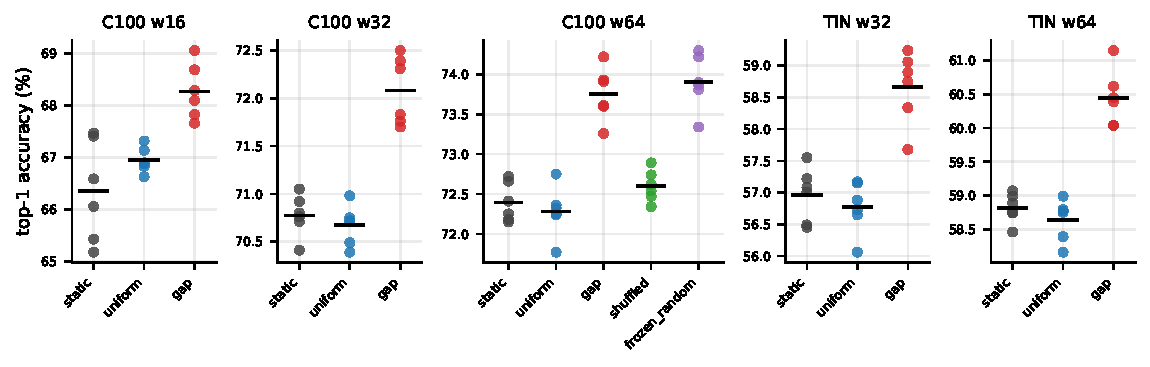
\includegraphics[width=\textwidth]{fig/g7_mb_allruns.pdf}
\caption{Every MobileNetV2 run at $K=4$ and $\tau=1$; bars are arm means.}
\label{fig:mballruns}
\end{figure}

\begin{table}[h]\centering\scriptsize
\caption{MobileNetV2, every run at $K=4$ and $\tau=1$: final-epoch top-1
accuracy (\si{\percent}). $^\dagger$ marks the run resumed after a CUDA
error.}
\label{tab:mballruns}
\begin{tabular}{l r l rrrrrr rr}
\toprule
dataset & width & arm & s0 & s1 & s2 & s3 & s4 & s5 & mean & sd \\
\midrule
CIFAR-100 & 16 & \texttt{static} & 65.43 & 67.41 & 66.59 & 65.18 & 67.47 & 66.06 & 66.357 & 0.973 \\
CIFAR-100 & 16 & \texttt{uniform} & 66.88 & 66.90 & 66.63 & 67.14 & 67.32 & 66.83 & 66.950 & 0.244 \\
CIFAR-100 & 16 & \texttt{gap} & 68.69 & 67.83 & 67.66 & 69.06 & 68.10 & 68.29 & 68.272 & 0.528 \\
CIFAR-100 & 32 & \texttt{static} & 70.92 & 71.05 & 70.71 & 70.80 & 70.41 & 70.76 & 70.775 & 0.217 \\
CIFAR-100 & 32 & \texttt{uniform} & 70.49 & 70.39 & 70.98 & 70.72 & 70.75 & 70.71 & 70.673 & 0.208 \\
CIFAR-100 & 32 & \texttt{gap} & 72.39 & 71.76 & 72.31 & 71.70 & 72.50 & 71.83 & 72.082 & 0.356 \\
CIFAR-100 & 64 & \texttt{static} & 72.66 & 72.18 & 72.15 & 72.25 & 72.41 & 72.72 & 72.395 & 0.246 \\
CIFAR-100 & 64 & \texttt{uniform} & 72.32 & 71.77 & 72.75 & 72.24 & 72.25 & 72.36 & 72.282 & 0.314 \\
CIFAR-100 & 64 & \texttt{gap} & 74.22 & 73.26 & 73.93 & 73.91 & 73.60 & 73.61 & 73.755 & 0.335 \\
CIFAR-100 & 64 & \texttt{shuffled} & 72.34 & 72.62 & 72.54 & 72.74 & 72.89 & 72.47 & 72.600 & 0.196 \\
CIFAR-100 & 64 & \texttt{frozen\_random} & 74.22 & 74.30 & 73.81 & 73.34 & 73.87 & 73.90 & 73.907 & 0.342 \\
Tiny-ImageNet & 32 & \texttt{static} & 57.01 & 57.08 & 56.45 & 57.22 & 56.49 & 57.55 & 56.967 & 0.427 \\
Tiny-ImageNet & 32 & \texttt{uniform} & 56.06 & 56.65 & 56.88 & 56.73 & 57.17 & 57.15 & 56.773 & 0.409 \\
Tiny-ImageNet & 32 & \texttt{gap} & 58.90 & 58.34 & 59.06 & 57.68 & 58.75 & 59.24 & 58.662 & 0.570 \\
Tiny-ImageNet & 64 & \texttt{static} & 59.07 & 58.99 & 58.89 & 58.74 & 58.75 & 58.46 & 58.817 & 0.218 \\
Tiny-ImageNet & 64 & \texttt{uniform} & 58.39 & 58.16 & 58.99 & 58.75 & 58.77 & 58.79 & 58.642 & 0.306 \\
Tiny-ImageNet & 64 & \texttt{gap} & 60.45 & 61.15$^\dagger$ & 60.04 & 60.62 & 60.04 & 60.39 & 60.448 & 0.414 \\
\bottomrule
\end{tabular}
\end{table}

\begin{table}[h]\centering\small
\caption{MobileNetV2: paired comparisons against \texttt{static}, $n=6$.}
\label{tab:mbvsstatic}
\resizebox{\textwidth}{!}{%
\begin{tabular}{l r l r l ll r l l}
\toprule
dataset & width & arm & $\Delta$ (pp) & \SI{95}{\percent} CI & $p_t$ & $p_W$ & $d_z$ & $p_{\text{TOST}}$ & verdict \\
\midrule
CIFAR-100 & 16 & \texttt{uniform} & +0.593 & [-0.425, +1.612] & 0.1945 & 0.3125 & +0.61 & 0.5884 & inconclusive \\
CIFAR-100 & 16 & \texttt{gap} & +1.915 & [+0.404, +3.426] & 0.0225 & 0.0312 & +1.33 & 0.9694 & higher \\
CIFAR-100 & 32 & \texttt{uniform} & -0.102 & [-0.510, +0.306] & 0.5501 & 0.5625 & -0.26 & 0.0269 & equivalent \\
CIFAR-100 & 32 & \texttt{gap} & +1.307 & [+0.771, +1.843] & 0.0015 & 0.0312 & +2.56 & 0.9941 & higher \\
CIFAR-100 & 64 & \texttt{uniform} & -0.113 & [-0.512, +0.285] & 0.4978 & 0.4375 & -0.30 & 0.0275 & equivalent \\
CIFAR-100 & 64 & \texttt{gap} & +1.360 & [+0.986, +1.734] & 0.0002 & 0.0312 & +3.82 & 0.9990 & higher \\
CIFAR-100 & 64 & \texttt{shuffled} & +0.205 & [-0.196, +0.606] & 0.2456 & 0.1562 & +0.54 & 0.0585 & inconclusive \\
CIFAR-100 & 64 & \texttt{frozen\_random} & +1.512 & [+1.123, +1.900] & 0.0002 & 0.0312 & +4.08 & 0.9994 & higher \\
Tiny-ImageNet & 32 & \texttt{uniform} & -0.193 & [-0.842, +0.455] & 0.4782 & 0.6250 & -0.31 & 0.1393 & inconclusive \\
Tiny-ImageNet & 32 & \texttt{gap} & +1.695 & [+0.895, +2.495] & 0.0028 & 0.0312 & +2.22 & 0.9939 & higher \\
Tiny-ImageNet & 64 & \texttt{uniform} & -0.175 & [-0.664, +0.314] & 0.4001 & 1.0000 & -0.38 & 0.0742 & inconclusive \\
Tiny-ImageNet & 64 & \texttt{gap} & +1.632 & [+1.201, +2.062] & 0.0002 & 0.0312 & +3.98 & 0.9995 & higher \\
\bottomrule
\end{tabular}}
\end{table}

\begin{table}[h]\centering\small
\caption{MobileNetV2: departure of each dynamic layer's router from
uniform, $10^3\,(1-\tilde H)$, mean over six seeds, $K=4$. Layers are
numbered from the input; a value of 0.00 is below $5\times10^{-6}$.}
\label{tab:mblayer}
\begin{tabular}{r rrrr rr r}
\toprule
& \multicolumn{4}{c}{CIFAR-100, width 64} & \multicolumn{2}{c}{CIFAR-100, width 16} & TIN w64 \\
\cmidrule(lr){2-5}\cmidrule(lr){6-7}\cmidrule(lr){8-8}
layer & \texttt{gap} & \texttt{gap} ann. & \texttt{frozen\_random} & \texttt{shuffled} & \texttt{gap} & \texttt{gap} ann. & \texttt{gap} \\
\midrule
1 & 3.66 & 4.15 & 4.23 & 0.11 & 7.79 & 16.51 & 1.87 \\
2 & 9.38 & 7.63 & 6.45 & 0.11 & 7.14 & 0.43 & 5.87 \\
3 & 9.54 & 0.00 & 2.46 & 0.01 & 7.31 & 0.00 & 9.59 \\
4 & 9.36 & 0.00 & 3.89 & 0.02 & 7.64 & 2.05 & 4.22 \\
5 & 6.34 & 0.00 & 6.19 & 0.02 & 0.37 & 0.00 & 0.90 \\
6 & 5.33 & 0.00 & 2.46 & 0.00 & 1.37 & 0.00 & 1.65 \\
7 & 26.08 & 0.00 & 4.94 & 0.02 & 9.49 & 0.00 & 7.38 \\
8 & 13.15 & 0.00 & 2.26 & 0.02 & 6.17 & 0.00 & 0.04 \\
9 & 9.26 & 0.00 & 1.80 & 0.00 & 0.00 & 0.00 & 4.38 \\
10 & 39.87 & 0.00 & 2.52 & 0.00 & 0.00 & 0.00 & 4.37 \\
11 & 29.20 & 0.00 & 3.18 & 0.27 & 19.95 & 0.00 & 15.63 \\
12 & 13.11 & 0.00 & 5.60 & 0.04 & 5.12 & 0.00 & 15.31 \\
13 & 5.94 & 0.00 & 1.68 & 0.00 & 4.54 & 0.00 & 15.55 \\
14 & 23.36 & 0.00 & 0.29 & 0.03 & 35.60 & 0.00 & 15.25 \\
15 & 8.10 & 0.00 & 1.40 & 0.20 & 7.85 & 0.00 & 22.07 \\
16 & 2.89 & 0.00 & 0.43 & 0.07 & 6.86 & 0.00 & 13.50 \\
17 & 9.83 & 0.00 & 0.24 & 0.00 & 15.80 & 0.00 & 5.21 \\
\midrule mean & 13.20 & 0.69 & 2.94 & 0.05 & 8.41 & 1.12 & 8.40 \\
\bottomrule
\end{tabular}
\end{table}

\begin{table}[h]\centering\small
\caption{MobileNetV2: configuration and cost. Parameters are counted from
the model definition; router parameters are in thousands (the frozen
router is held as buffers and not counted). Training loss is the
final-epoch mean over six seeds; minutes are logged wall-clock time.}
\label{tab:mbconfig}
\begin{tabular}{l r l rr r r}
\toprule
dataset & width & arm & params (M) & router (K) & train loss & min/run \\
\midrule
CIFAR-100 & 16 & \texttt{static} & 0.37 & 0.0 & 0.729 & 16.2 \\
CIFAR-100 & 16 & \texttt{uniform} & 0.42 & 0.0 & 0.717 & 20.2 \\
CIFAR-100 & 16 & \texttt{gap} & 0.49 & 75.3 & 0.655 & 41.0 \\
CIFAR-100 & 32 & \texttt{static} & 0.82 & 0.0 & 0.409 & 18.0 \\
CIFAR-100 & 32 & \texttt{uniform} & 0.91 & 0.0 & 0.418 & 21.6 \\
CIFAR-100 & 32 & \texttt{gap} & 1.20 & 289.1 & 0.344 & 47.3 \\
CIFAR-100 & 64 & \texttt{static} & 2.35 & 0.0 & 0.248 & 24.8 \\
CIFAR-100 & 64 & \texttt{uniform} & 2.54 & 0.0 & 0.231 & 26.9 \\
CIFAR-100 & 64 & \texttt{gap} & 3.68 & 1137.3 & 0.168 & 78.1 \\
CIFAR-100 & 64 & \texttt{shuffled} & 3.68 & 1137.3 & 0.229 & 92.0 \\
CIFAR-100 & 64 & \texttt{frozen\_random} & 2.54 & 0.0 & 0.175 & 77.4 \\
Tiny-ImageNet & 32 & \texttt{static} & 0.94 & 0.0 & 1.345 & 116.1 \\
Tiny-ImageNet & 32 & \texttt{uniform} & 1.04 & 0.0 & 1.359 & 114.5 \\
Tiny-ImageNet & 32 & \texttt{gap} & 1.33 & 289.1 & 1.220 & 340.6 \\
Tiny-ImageNet & 64 & \texttt{static} & 2.48 & 0.0 & 1.138 & 187.4 \\
Tiny-ImageNet & 64 & \texttt{uniform} & 2.67 & 0.0 & 1.126 & 191.3 \\
Tiny-ImageNet & 64 & \texttt{gap} & 3.81 & 1137.3 & 0.995 & 792.5 \\
\bottomrule
\end{tabular}
\end{table}

\begin{table}[h]\centering\small
\caption{Every MobileNetV2 run. GPU-hours are from logged wall-clock time.}
\label{tab:mbinvent}
\begin{tabular}{l r r l l r r}
\toprule
dataset & width & $K$ & $\tau$ & arms & runs & GPU-h \\
\midrule
CIFAR-100 & 16 & 4 & constant & \texttt{static}, \texttt{uniform}, \texttt{gap} & 18 & 7.7 \\
CIFAR-100 & 32 & 4 & constant & \texttt{static}, \texttt{uniform}, \texttt{gap} & 18 & 8.7 \\
CIFAR-100 & 64 & 4 & constant & \texttt{static}, \texttt{uniform}, \texttt{gap}, \texttt{shuffled}, \texttt{frozen\_random} & 30 & 29.9 \\
CIFAR-100 & 32 & 2 & constant & \texttt{gap} & 6 & 5.2 \\
CIFAR-100 & 32 & 8 & constant & \texttt{gap} & 6 & 9.9 \\
CIFAR-100 & 16 & 4 & annealed & \texttt{gap} & 6 & 4.1 \\
CIFAR-100 & 32 & 4 & annealed & \texttt{gap} & 6 & 4.7 \\
CIFAR-100 & 64 & 4 & annealed & \texttt{gap} & 6 & 9.1 \\
Tiny-ImageNet & 32 & 4 & constant & \texttt{static}, \texttt{uniform}, \texttt{gap} & 18 & 57.1 \\
Tiny-ImageNet & 64 & 4 & constant & \texttt{static}, \texttt{uniform}, \texttt{gap} & 18 & 117.1 \\
\midrule \multicolumn{5}{l}{total} & 132 & 253.6 \\
\bottomrule
\end{tabular}
\end{table}

\clearpage
\section{Complete results: VGG-16}

\begin{figure}[h]\centering
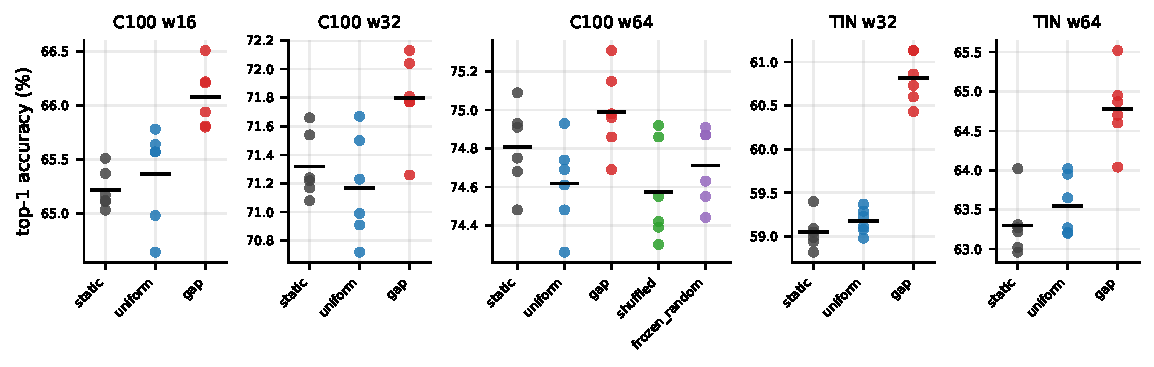
\includegraphics[width=\textwidth]{fig/g9_vg_allruns.pdf}
\caption{Every VGG-16 run at $K=4$ and $\tau=1$; bars are arm means.}
\label{fig:vgallruns}
\end{figure}

\begin{table}[h]\centering\scriptsize
\caption{VGG-16, every run at $K=4$ and $\tau=1$: final-epoch top-1
accuracy (\si{\percent}). $^\dagger$ marks the run resumed after an
interruption.}
\label{tab:vgallruns}
\begin{tabular}{l r l rrrrrr rr}
\toprule
dataset & width & arm & s0 & s1 & s2 & s3 & s4 & s5 & mean & sd \\
\midrule
CIFAR-100 & 16 & \texttt{static} & 65.03 & 65.37 & 65.12 & 65.17 & 65.51 & 65.11 & 65.218 & 0.183 \\
CIFAR-100 & 16 & \texttt{uniform} & 64.64 & 65.78 & 65.57 & 65.64 & 64.98 & 65.57 & 65.363 & 0.448 \\
CIFAR-100 & 16 & \texttt{gap} & 66.22 & 65.81 & 66.51 & 65.80 & 66.21 & 65.94 & 66.082 & 0.280 \\
CIFAR-100 & 32 & \texttt{static} & 71.17 & 71.66 & 71.24 & 71.22 & 71.54 & 71.08 & 71.318 & 0.228 \\
CIFAR-100 & 32 & \texttt{uniform} & 70.91 & 70.99 & 71.67 & 71.23 & 70.72 & 71.50 & 71.170 & 0.365 \\
CIFAR-100 & 32 & \texttt{gap} & 72.04 & 71.81 & 71.77 & 71.77 & 72.13 & 71.26 & 71.797 & 0.303 \\
CIFAR-100 & 64 & \texttt{static} & 74.68 & 74.91 & 75.09 & 74.75 & 74.93 & 74.48 & 74.807 & 0.215 \\
CIFAR-100 & 64 & \texttt{uniform} & 74.26 & 74.48 & 74.93 & 74.61 & 74.69 & 74.74 & 74.618 & 0.230 \\
CIFAR-100 & 64 & \texttt{gap} & 74.69 & 74.96 & 75.15 & 74.86 & 75.31 & 74.98 & 74.992 & 0.217 \\
CIFAR-100 & 64 & \texttt{shuffled} & 74.55$^\dagger$ & 74.30 & 74.86 & 74.42 & 74.39 & 74.92 & 74.573 & 0.259 \\
CIFAR-100 & 64 & \texttt{frozen\_random} & 74.63 & 74.44 & 74.87 & 74.87 & 74.55 & 74.91 & 74.712 & 0.198 \\
Tiny-ImageNet & 32 & \texttt{static} & 58.94 & 59.40 & 58.82 & 59.05 & 58.99 & 59.09 & 59.048 & 0.196 \\
Tiny-ImageNet & 32 & \texttt{uniform} & 59.23 & 59.37 & 59.29 & 58.98 & 59.11 & 59.08 & 59.177 & 0.145 \\
Tiny-ImageNet & 32 & \texttt{gap} & 61.13 & 60.60 & 60.73 & 61.13 & 60.43 & 60.86 & 60.813 & 0.284 \\
Tiny-ImageNet & 64 & \texttt{static} & 63.02 & 63.27 & 63.31 & 62.96 & 63.22 & 64.02 & 63.300 & 0.379 \\
Tiny-ImageNet & 64 & \texttt{uniform} & 63.20 & 64.02 & 63.21 & 63.95 & 63.27 & 63.65 & 63.550 & 0.376 \\
Tiny-ImageNet & 64 & \texttt{gap} & 64.87 & 64.60 & 65.52 & 64.95 & 64.04 & 64.70 & 64.780 & 0.484 \\
\bottomrule
\end{tabular}
\end{table}

\begin{table}[h]\centering\small
\caption{VGG-16: paired comparisons against \texttt{static}, $n=6$.}
\label{tab:vgvsstatic}
\resizebox{\textwidth}{!}{%
\begin{tabular}{l r l r l ll r l l}
\toprule
dataset & width & arm & $\Delta$ (pp) & \SI{95}{\percent} CI & $p_t$ & $p_W$ & $d_z$ & $p_{\text{TOST}}$ & verdict \\
\midrule
CIFAR-100 & 16 & \texttt{uniform} & +0.145 & [-0.349, +0.639] & 0.4849 & 0.5625 & +0.31 & 0.0621 & inconclusive \\
CIFAR-100 & 16 & \texttt{gap} & +0.863 & [+0.486, +1.240] & 0.0020 & 0.0312 & +2.40 & 0.9720 & higher \\
CIFAR-100 & 32 & \texttt{uniform} & -0.148 & [-0.707, +0.411] & 0.5254 & 0.6875 & -0.28 & 0.0834 & inconclusive \\
CIFAR-100 & 32 & \texttt{gap} & +0.478 & [+0.193, +0.764] & 0.0077 & 0.0312 & +1.76 & 0.4265 & higher \\
CIFAR-100 & 64 & \texttt{uniform} & -0.188 & [-0.453, +0.077] & 0.1273 & 0.2188 & -0.75 & 0.0147 & equivalent \\
CIFAR-100 & 64 & \texttt{gap} & +0.185 & [-0.029, +0.399] & 0.0766 & 0.0312 & +0.91 & 0.0064 & equivalent \\
CIFAR-100 & 64 & \texttt{shuffled} & -0.233 & [-0.629, +0.162] & 0.1896 & 0.2188 & -0.62 & 0.0717 & inconclusive \\
CIFAR-100 & 64 & \texttt{frozen\_random} & -0.095 & [-0.447, +0.257] & 0.5183 & 0.5625 & -0.28 & 0.0157 & equivalent \\
Tiny-ImageNet & 32 & \texttt{uniform} & +0.128 & [-0.095, +0.352] & 0.1997 & 0.4375 & +0.60 & 0.0039 & equivalent \\
Tiny-ImageNet & 32 & \texttt{gap} & +1.765 & [+1.365, +2.165] & $<10^{-4}$ & 0.0312 & +4.63 & 0.9998 & higher \\
Tiny-ImageNet & 64 & \texttt{uniform} & +0.250 & [-0.295, +0.795] & 0.2915 & 0.4375 & +0.48 & 0.1458 & inconclusive \\
Tiny-ImageNet & 64 & \texttt{gap} & +1.480 & [+0.812, +2.148] & 0.0023 & 0.0312 & +2.32 & 0.9935 & higher \\
\bottomrule
\end{tabular}}
\end{table}

\begin{table}[h]\centering\small
\caption{VGG-16: configuration and cost. Parameters are counted from the
model definition and equal the counts the training log prints; router
parameters are in thousands (the frozen router is held as buffers and not
counted). Training loss is the final-epoch mean over six seeds; minutes
are logged wall-clock time.}
\label{tab:vgconfig}
\begin{tabular}{l r l rr r r}
\toprule
dataset & width & arm & params (M) & router (K) & train loss & min/run \\
\midrule
CIFAR-100 & 16 & \texttt{static} & 0.93 & 0.0 & 0.1025 & 6.8 \\
CIFAR-100 & 16 & \texttt{uniform} & 3.69 & 0.0 & 0.1040 & 9.0 \\
CIFAR-100 & 16 & \texttt{gap} & 3.72 & 26.5 & 0.0935 & 25.4 \\
CIFAR-100 & 32 & \texttt{static} & 3.71 & 0.0 & 0.0148 & 6.9 \\
CIFAR-100 & 32 & \texttt{uniform} & 14.74 & 0.0 & 0.0152 & 9.0 \\
CIFAR-100 & 32 & \texttt{gap} & 14.84 & 99.7 & 0.0145 & 26.0 \\
CIFAR-100 & 64 & \texttt{static} & 14.77 & 0.0 & 0.0053 & 10.6 \\
CIFAR-100 & 64 & \texttt{uniform} & 58.90 & 0.0 & 0.0058 & 19.8 \\
CIFAR-100 & 64 & \texttt{gap} & 59.29 & 391.8 & 0.0057 & 51.1 \\
CIFAR-100 & 64 & \texttt{shuffled} & 59.29 & 391.8 & 0.0060 & 58.3 \\
CIFAR-100 & 64 & \texttt{frozen\_random} & 58.90 & 0.0 & 0.0060 & 50.1 \\
Tiny-ImageNet & 32 & \texttt{static} & 3.73 & 0.0 & 0.0713 & 28.0 \\
Tiny-ImageNet & 32 & \texttt{uniform} & 14.77 & 0.0 & 0.0720 & 31.7 \\
Tiny-ImageNet & 32 & \texttt{gap} & 14.86 & 99.7 & 0.0313 & 115.5 \\
Tiny-ImageNet & 64 & \texttt{static} & 14.82 & 0.0 & 0.0112 & 63.7 \\
Tiny-ImageNet & 64 & \texttt{uniform} & 58.95 & 0.0 & 0.0120 & 79.8 \\
Tiny-ImageNet & 64 & \texttt{gap} & 59.34 & 391.8 & 0.0110 & 307.3 \\
\bottomrule
\end{tabular}
\end{table}

\begin{table}[h]\centering\small
\caption{Every VGG-16 run. GPU-hours are from logged wall-clock time.}
\label{tab:vginvent}
\begin{tabular}{l r r l l r r}
\toprule
dataset & width & $K$ & $\tau$ & arms & runs & GPU-h \\
\midrule
CIFAR-100 & 16 & 4 & constant & \texttt{static}, \texttt{uniform}, \texttt{gap} & 18 & 4.1 \\
CIFAR-100 & 32 & 4 & constant & \texttt{static}, \texttt{uniform}, \texttt{gap} & 18 & 4.2 \\
CIFAR-100 & 64 & 4 & constant & \texttt{static}, \texttt{uniform}, \texttt{gap}, \texttt{shuffled}, \texttt{frozen\_random} & 30 & 19.0 \\
CIFAR-100 & 32 & 2 & constant & \texttt{gap} & 6 & 2.0 \\
CIFAR-100 & 32 & 8 & constant & \texttt{gap} & 6 & 4.1 \\
CIFAR-100 & 16 & 4 & annealed & \texttt{gap} & 6 & 2.5 \\
CIFAR-100 & 32 & 4 & annealed & \texttt{gap} & 6 & 2.6 \\
CIFAR-100 & 64 & 4 & annealed & \texttt{gap} & 6 & 5.1 \\
Tiny-ImageNet & 32 & 4 & constant & \texttt{static}, \texttt{uniform}, \texttt{gap} & 18 & 17.5 \\
Tiny-ImageNet & 64 & 4 & constant & \texttt{static}, \texttt{uniform}, \texttt{gap} & 18 & 45.1 \\
\midrule \multicolumn{5}{l}{total} & 132 & 106.2 \\
\bottomrule
\end{tabular}
\end{table}

\end{document}
